
\section{Experiments}\label{eval}
First, the experiments evaluate how various types of corrupted data benefit from data cleaning.
Next, the experiments explore different prioritization and model update schemes for progressive data cleaning.
Finally, \sys is evaluated end-to-end in a number of real-world data cleaning scenarios.

\subsection{Experimental Setup and Notation}
The main metric for evaluation is a relative measure of the trained model and the model if all of the data is cleaned.

\vspace{0.5em}

\noindent\textbf{Relative Model Error. } Let $\theta$ be the model trained on the dirty data, and let $\theta^*$ be the model trained on the same data if it was cleaned. Then the model error is defined as $\frac{\|\theta - \theta^*\|}{\|\theta^*\|}$.

\subsubsection{Scenarios}
%\vspace{0.5em}

%\noindent\textbf{Housing: } In this dataset, our task is to predict housing prices from 13 numerical and categorical covariates. There are 550 data points in this dataset. The model is a Logistic Regression classifier which predicts if the house price is greater than \$500k.

\vspace{0.25em}

\noindent\textbf{Income Classification (Adult): } In this dataset of 45,552 records, the task is to predict the income bracket (binary) from 12 numerical and categorical covariates with an SVM classifier. 

\vspace{0.25em}

\noindent\textbf{Seizure Classification (EEG): } In this dataset, the task is to predict the onset of a seizure (binary) from 15 numerical covariates with a thresholded Linear Regression. There are 14980 data points in this dataset. This classification task is inherently hard with an accuracy on completely clean data of only 65\%.

\vspace{0.25em}

\noindent\textbf{Handwriting Recognition (MNIST) \footnote{\scriptsize\url{http://ufldl.stanford.edu/wiki/index.php/Using_the_MNIST_Dataset}}: } In this dataset, the task is to classify 60,000 images of handwritten images into 10 categories with an one-to-all multiclass SVM classifier. The unique part of this dataset is the featurized data consists of a 784 dimensional vector which includes edge detectors and raw image patches. 

\vspace{0.25em}

\noindent\textbf{Dollars For Docs: } The dataset has 240,089 records with 5 textual attributes and one numerical attribute.
The dataset is featurized with bag-of-words featurization model for the textual attributes which resulted in a 2021 dimensional feature vector, and a binary SVM is used to classify the status of the medical donations.

\subsubsection{Compared Algorithms}
\noindent Here are the alternative methodologies evaluated in the experiments:

\vspace{0.25em}

\noindent\textbf{Robust Logistic Regression \cite{feng2014robust}. } Feng et al. proposed a variant of logistic regression that is robust to outliers. We chose this algorithm because it is a robust extension of the convex regularized loss model, leading to a better apples-to-apples comparison between the techniques. (See details in Appendix \ref{rlogit})  

\vspace{0.25em}

\noindent\textbf{Discarding Dirty Data. } As a baseline, dirty data is discarded.

\vspace{0.25em}

\noindent\textbf{SampleClean (SC) \cite{wang1999sample}. } SampleClean takes a sample of data, applies data cleaning, and then trains a model to completion on the sample.

\vspace{0.25em}

\noindent\textbf{Active Learning (AL) \cite{guillory2009active}. } An Active Learning algorithm that integrates with stochastic optimization (See details in Appendix \ref{al}). 

\vspace{0.25em}

\noindent\textbf{ActiveClean Oracle (AC+O): } In \sys Oracle, instead of an estimation step, the true clean value is used to evaluate the theoretical ideal performance of \sys.

\subsection{Does Data Cleaning Matter?}
The first experiment evaluates the benefits of data cleaning on two of the example datasets (EEG and Adult).
This is done without sampling to understand which types of data corruption are amenable to data cleaning and which are better suited for robust statistical techniques.
The experiment compares four schemes: (1) full data cleaning  , (2) baseline of no cleaning, (3) discarding the dirty data, and (4) robust logistic regression,. We corrupted 5\% of the training examples in each dataset in two different ways:

\vspace{0.5em}

\noindent\textbf{Random Corruption: } Simulated high-magnitude random outliers. 5\% of the examples are selected at random and a random feature is replaced with 3 times the highest feature value.

\vspace{0.5em}

\noindent\textbf{Systematic Corruption: } Simulated innocuous looking (but still incorrect) systematic corruption. The model is trained on the clean data, and the three most important features (highest weighted) are identified. The examples are sorted by each of these features and the top examples are corrupted with the mean value for that feature (5\% corruption in all). 
It is important to note that examples can have multiple corrupted features.

\begin{figure}[t]
\centering
 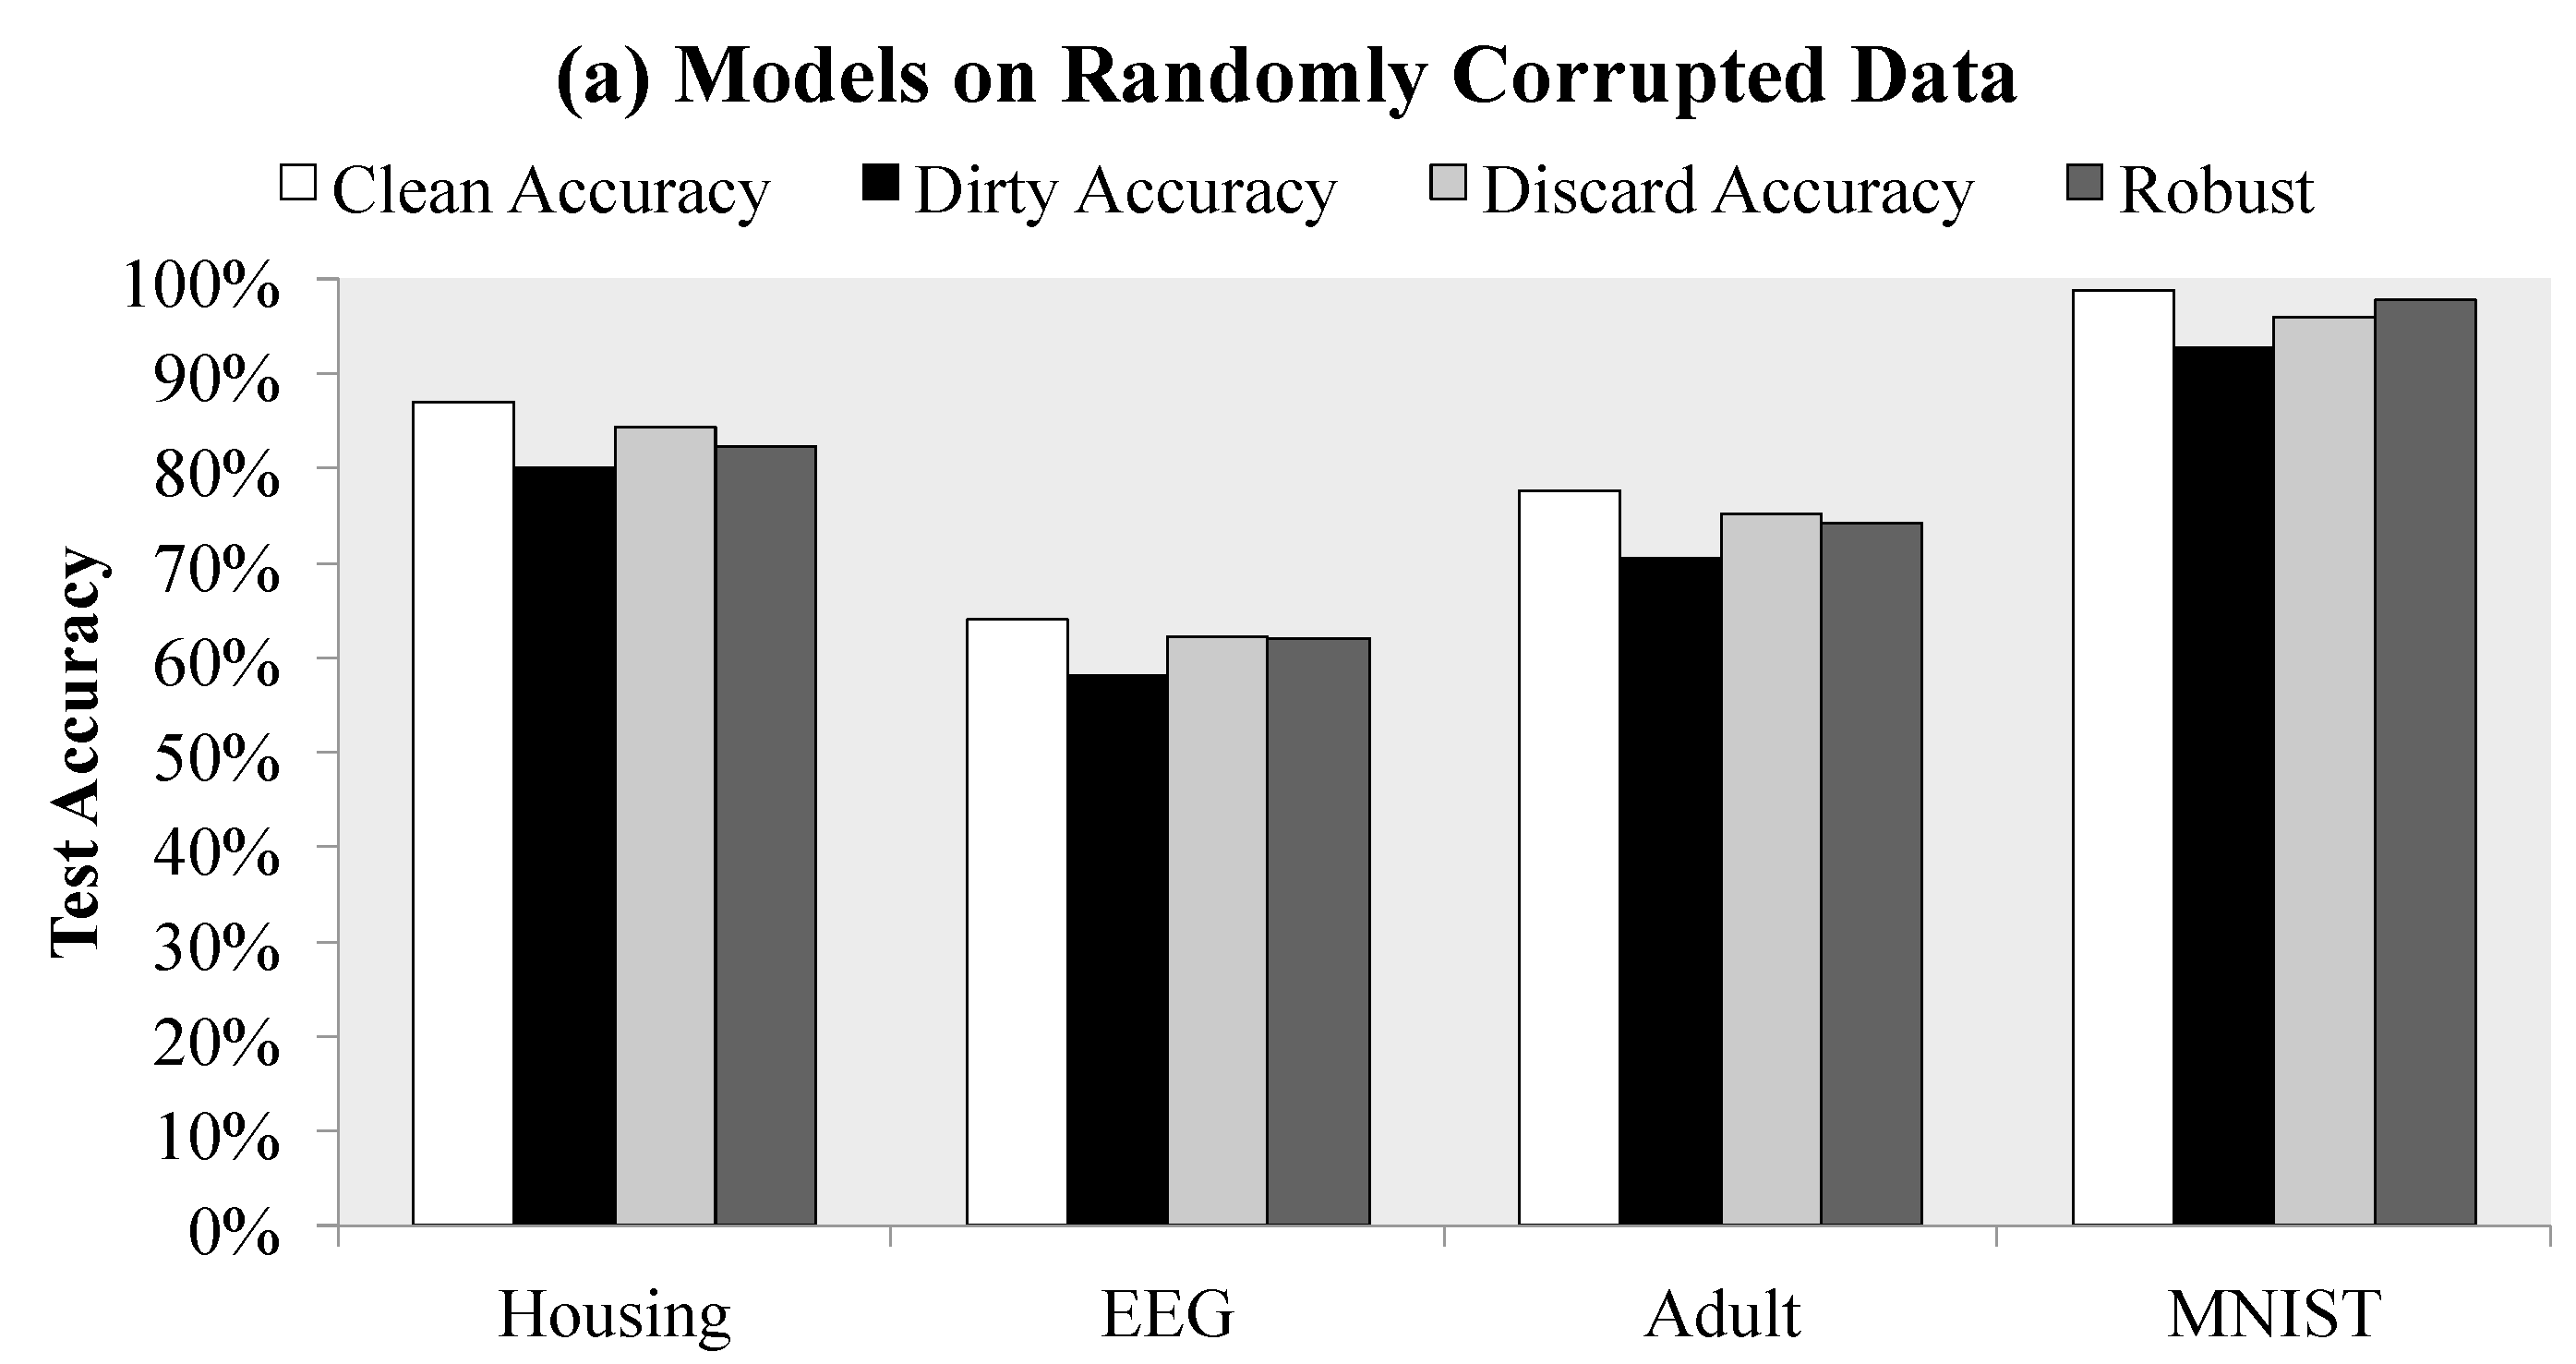
\includegraphics[width=0.49\columnwidth]{exp/exp2.pdf}
 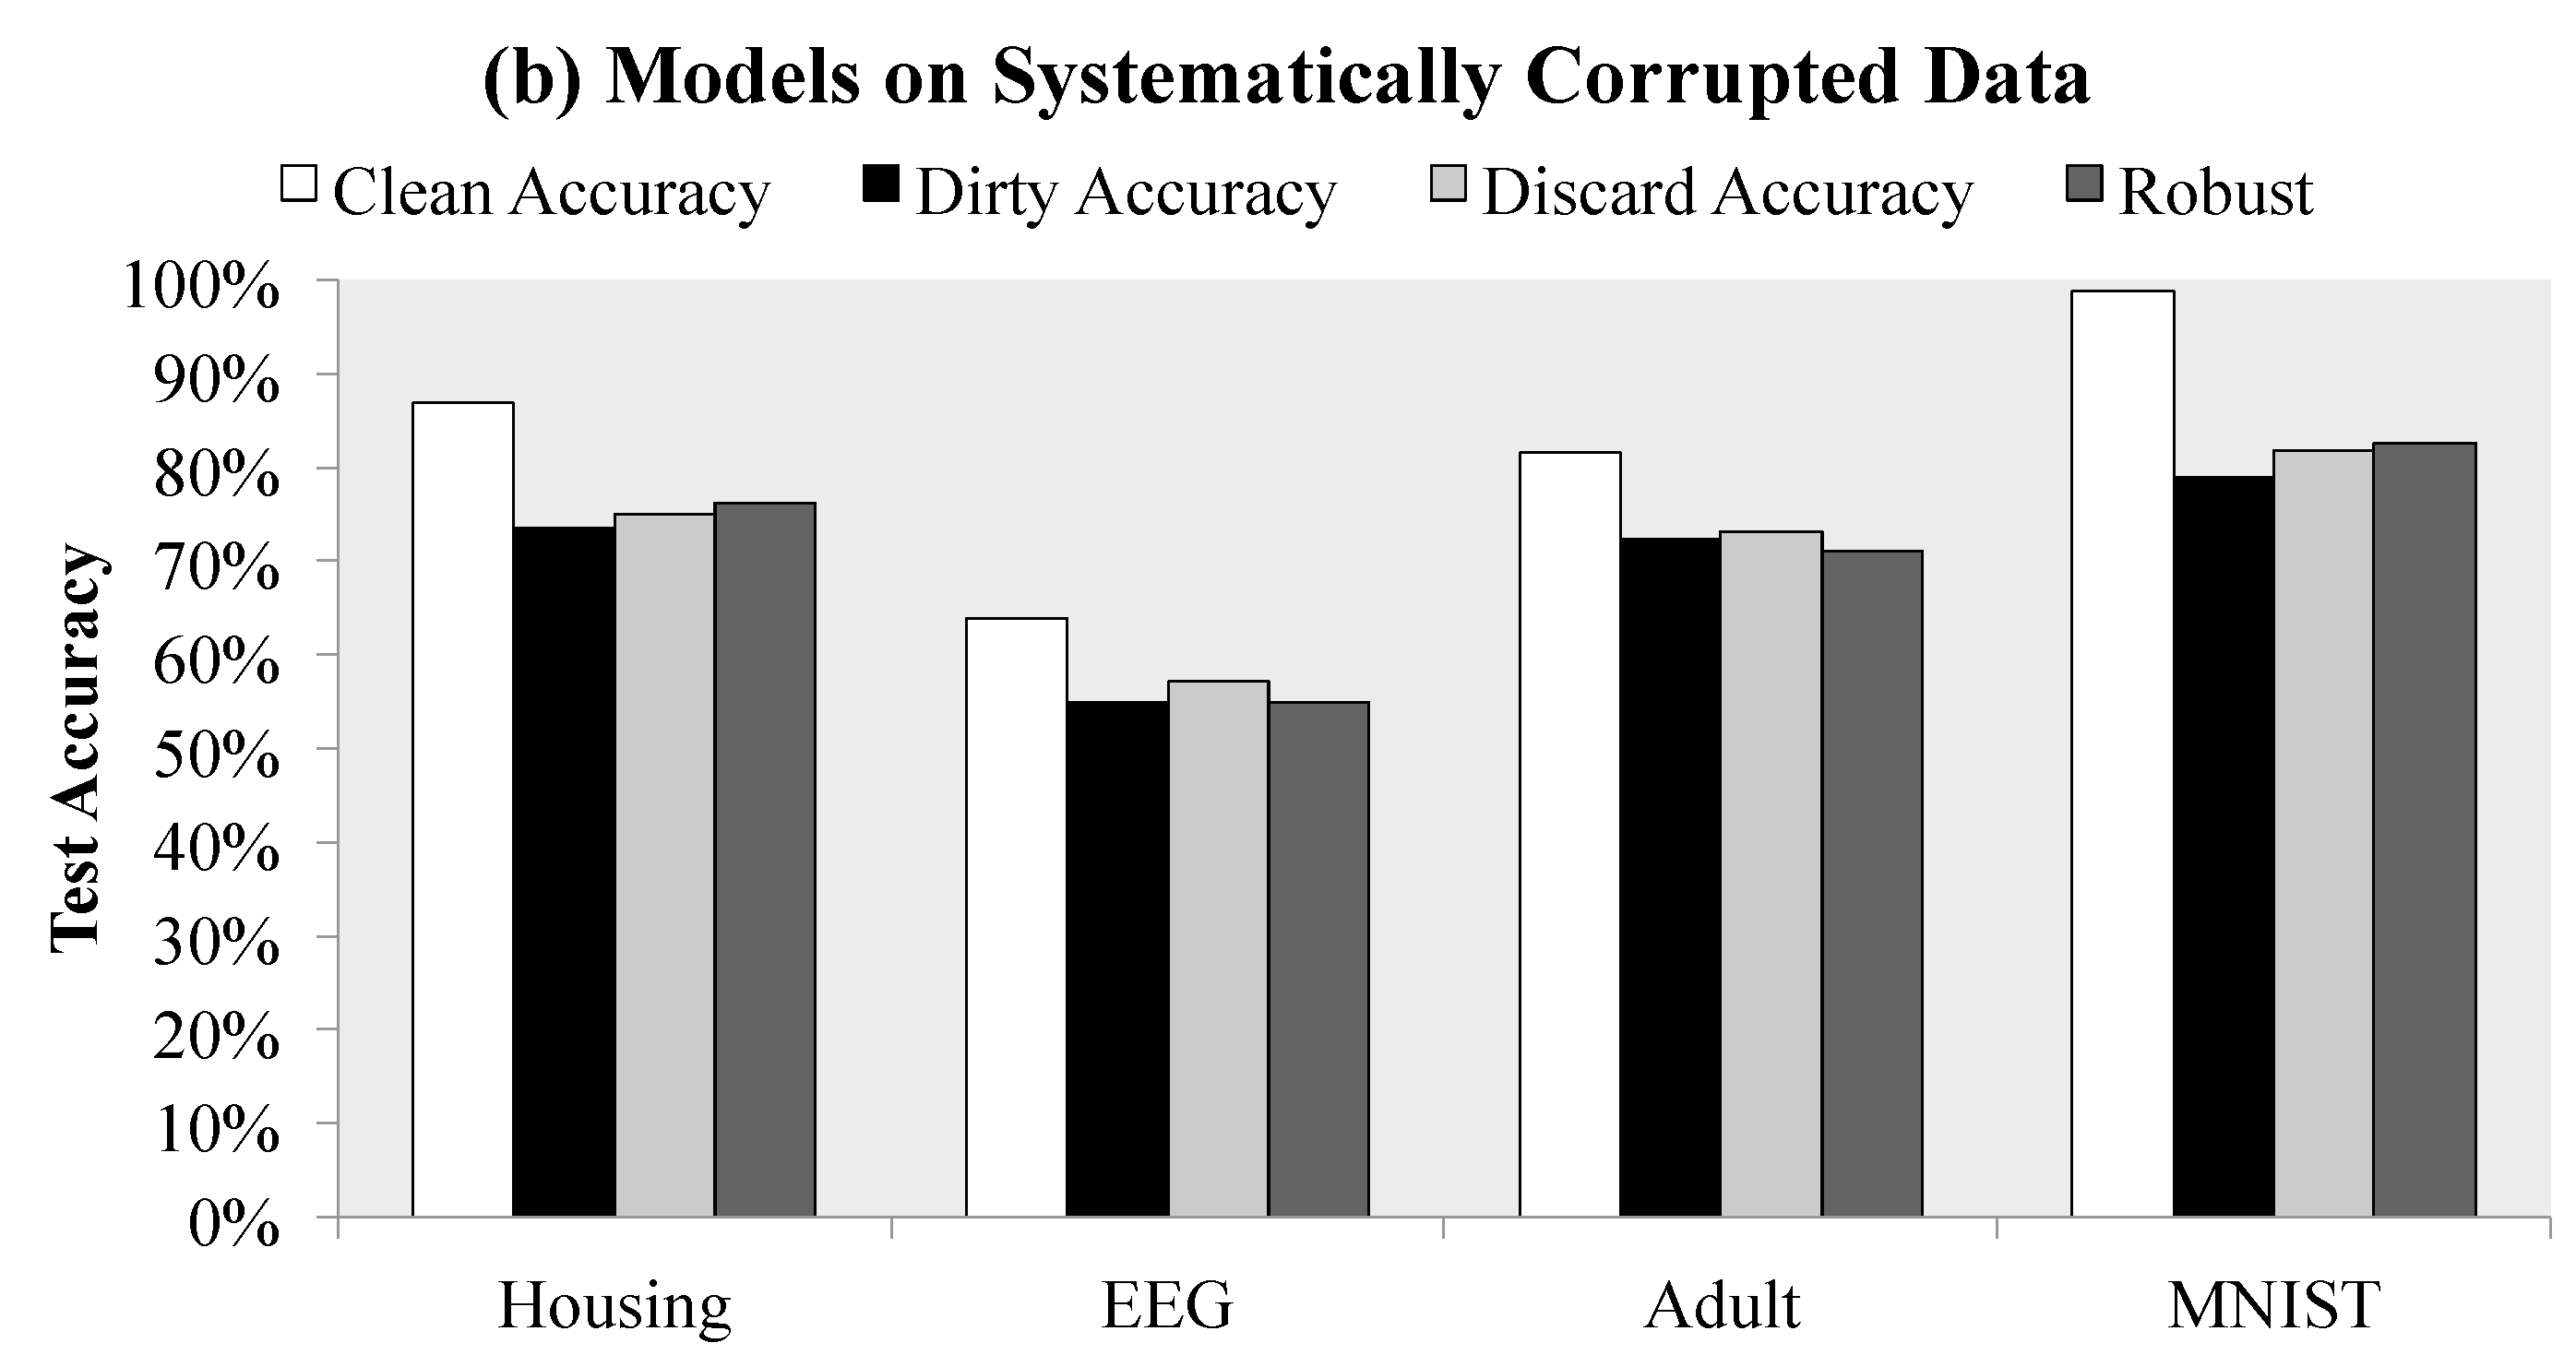
\includegraphics[width=0.49\columnwidth]{exp/exp1.pdf}
 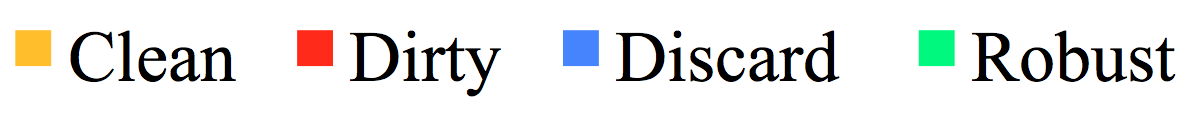
\includegraphics[width=0.5\columnwidth]{exp/legend-1.png}\vspace{-1em}
 \caption{(a) Robust techniques and discarding data work when corrupted data are random and look atypical. (b) Data cleaning can provide reliable performance in both the systematically corrupted setting and randomly corrupted setting.\label{sys-rand}}
\end{figure}

Figure \ref{sys-rand} shows the test accuracy for models trained on both types of data with the different techniques.
The robust method performs well on the random high-magnitude outliers with only a 2.0\% reduction in clean test accuracy for EEG and 2.5\% reduction for Adult.
In the random setting, discarding dirty data also performs relatively well.
However, the robust method falters on the systematic corruption with a 9.1\% reduction in clean test accuracy for EEG and 10.5\% reduction for Adult.
%Data cleaning is the most reliable option across datasets and corruption types.
The problem is that without cleaning, there is no way to know if the corruption is random or systematic and when to trust a robust method.
While data cleaning requires more effort, it provides benefits in both settings.
In the remaining experiments, unless otherwise noted, the experiments use systematic corruption.

\noindent \emph{Summary: A 5\% systematic corruption can introduce a 10\% reduction in test accuracy even when using a robust method.}

\subsection{\sys: A Priori Detection}
The next set of experiments evaluate different approaches to cleaning a sample of data compared to \sys using \emph{a priori} detection.
\emph{A priori} detection assumes that all of the corrupted records are known in advance but their clean values are unknown. 

\subsubsection{Active Learning and SampleClean}
The next experiment evaluates the samples-to-error tradeoff between four alternative algorithms: \sys (AC), SampleClean, Active Learning, and \sys+Oracle (AC+O).
Figure \ref{prio-perf} shows the model error and test accuracy as a function of the number of cleaned records.
In terms of model error, \sys gives its largest benefits for small sample sizes.
For 500 cleaned records of the Adult dataset, \sys has 6.1x less error than SampleClean and 2.1x less error than Active Learning.
For 500 cleaned records of the EEG dataset, \sys has 9.6x less error than SampleClean and 2.4x less error than Active Learning.
Both Active Learning and \sys benefit from the initialization with the dirty model as they do not retrain their models from scratch, and \sys improves on this performance with detection and error estimation.
These gains also correlate well to improvements in test accuracy.
For example, to achieve a test error of 1\% on the Adult dataset, \sys cleans 500 fewer records than Active Learning.


\vspace{0.25em}

\noindent \emph{Summary: \sys with a priori detection returns results that are more than 6x more accurate than SampleClean and 2x more accurate than Active Learning for cleaning 500 records.}

\begin{figure}[t]
\centering\vspace{-1em}
 %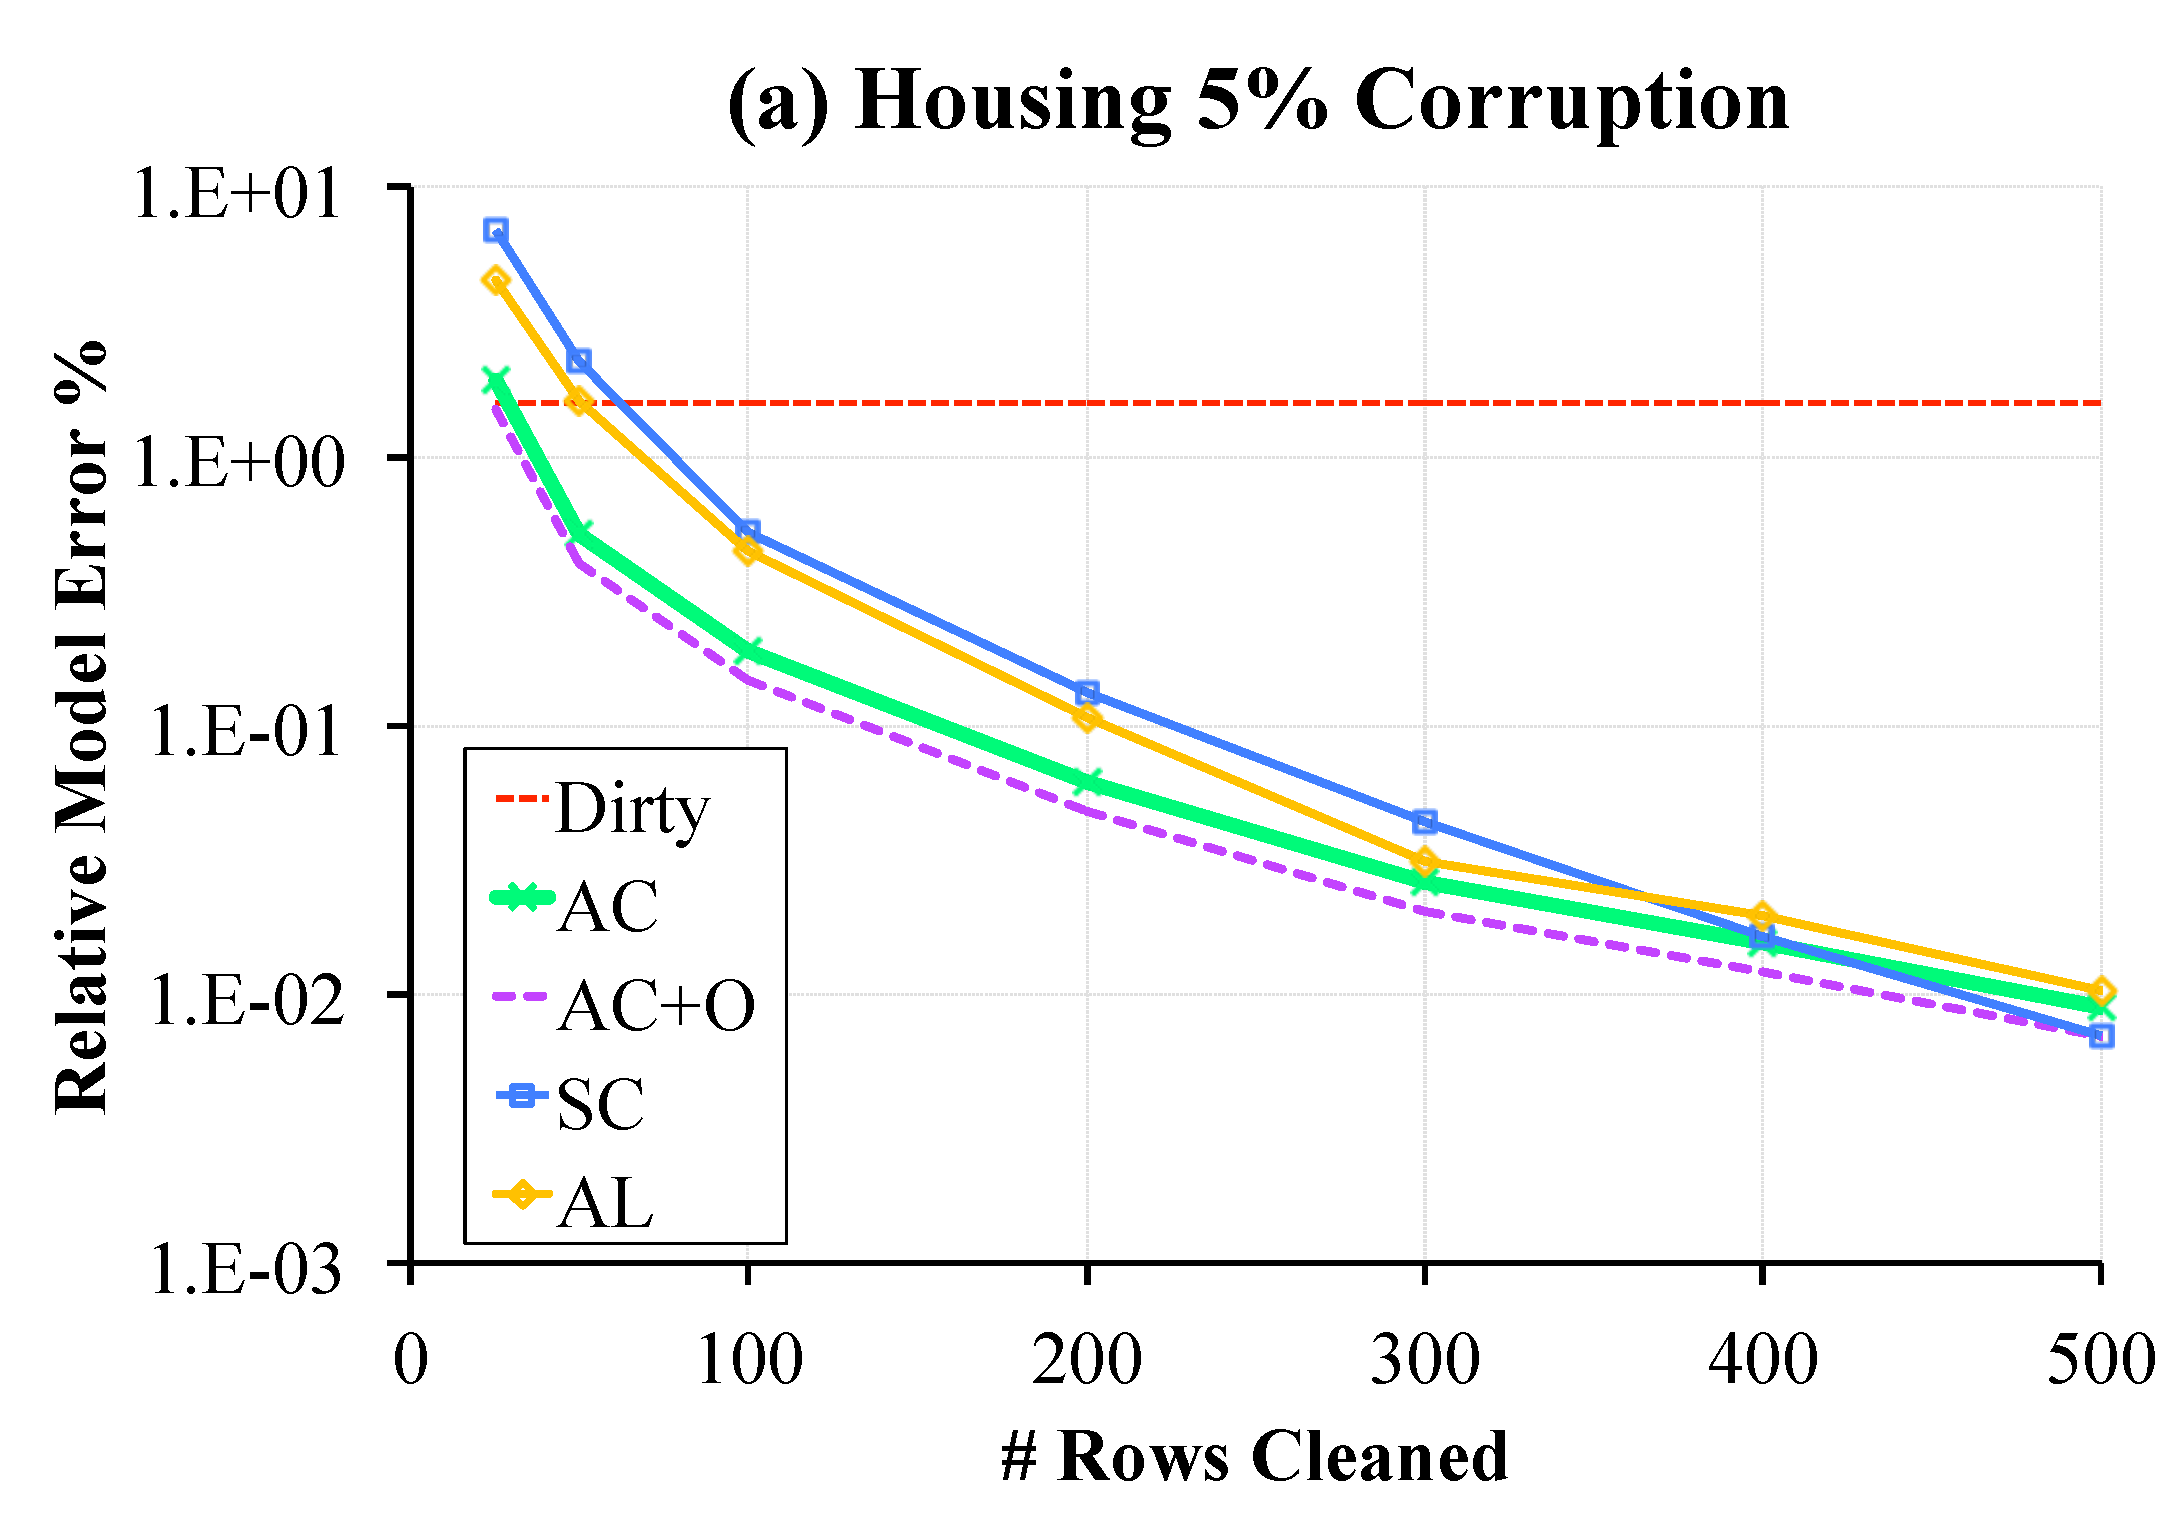
\includegraphics[scale=0.15]{exp/exp3a.pdf}
 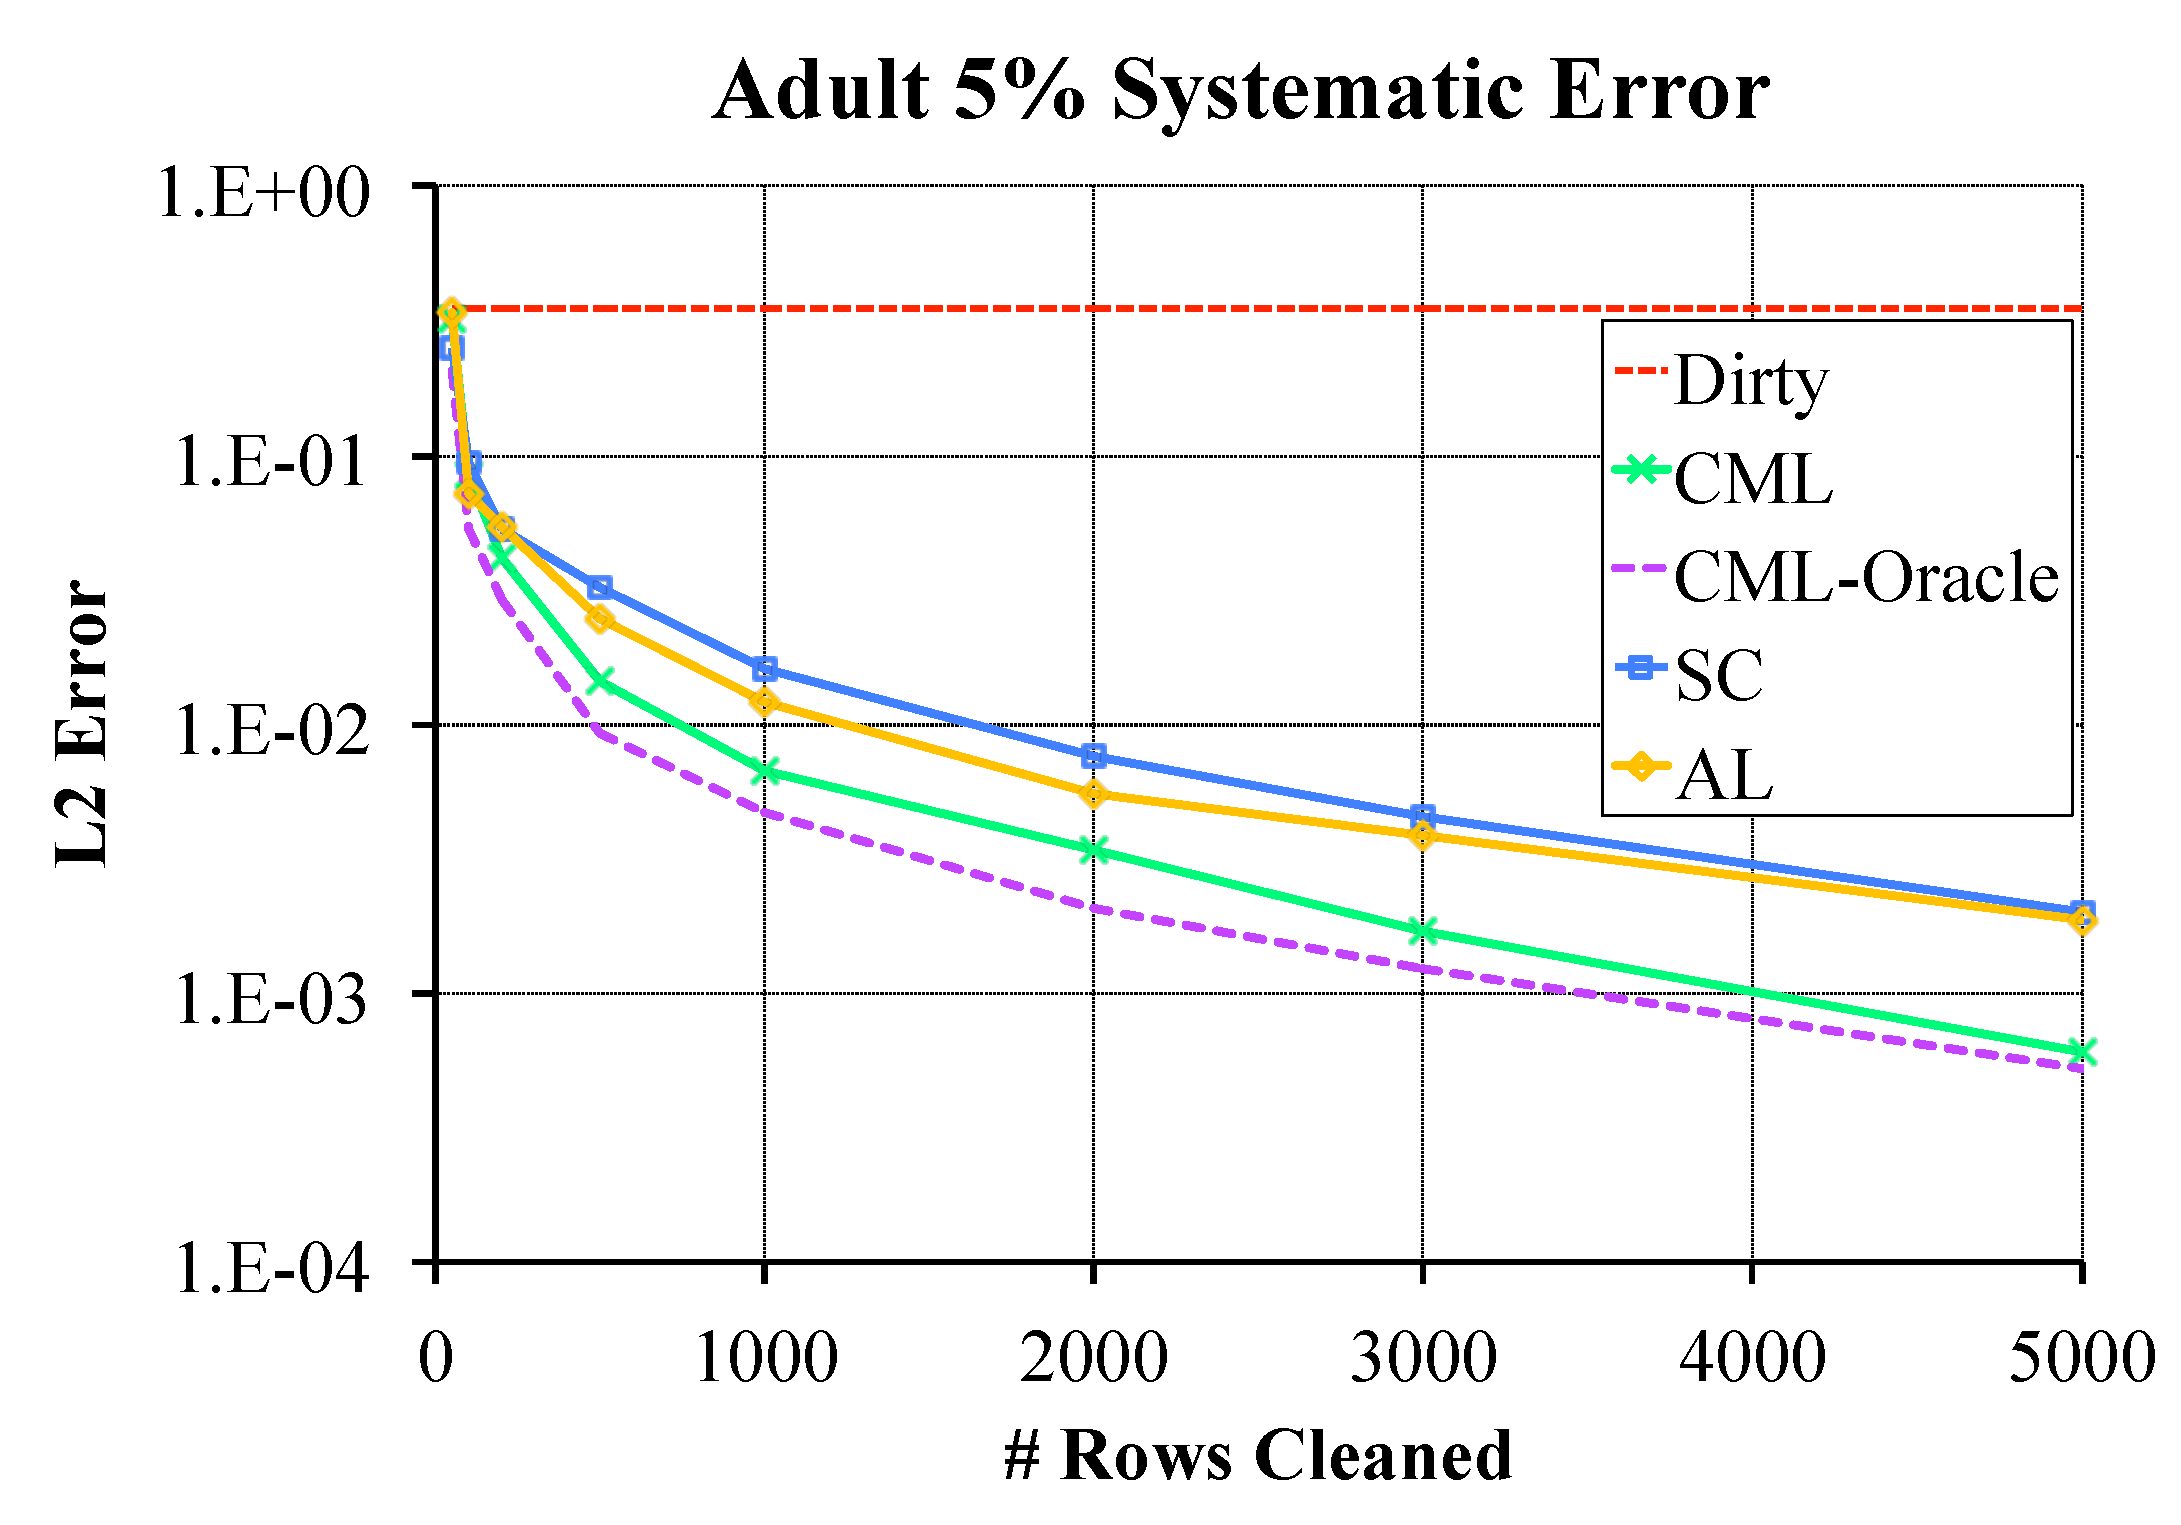
\includegraphics[width=0.49\columnwidth]{exp/exp3b.pdf}
  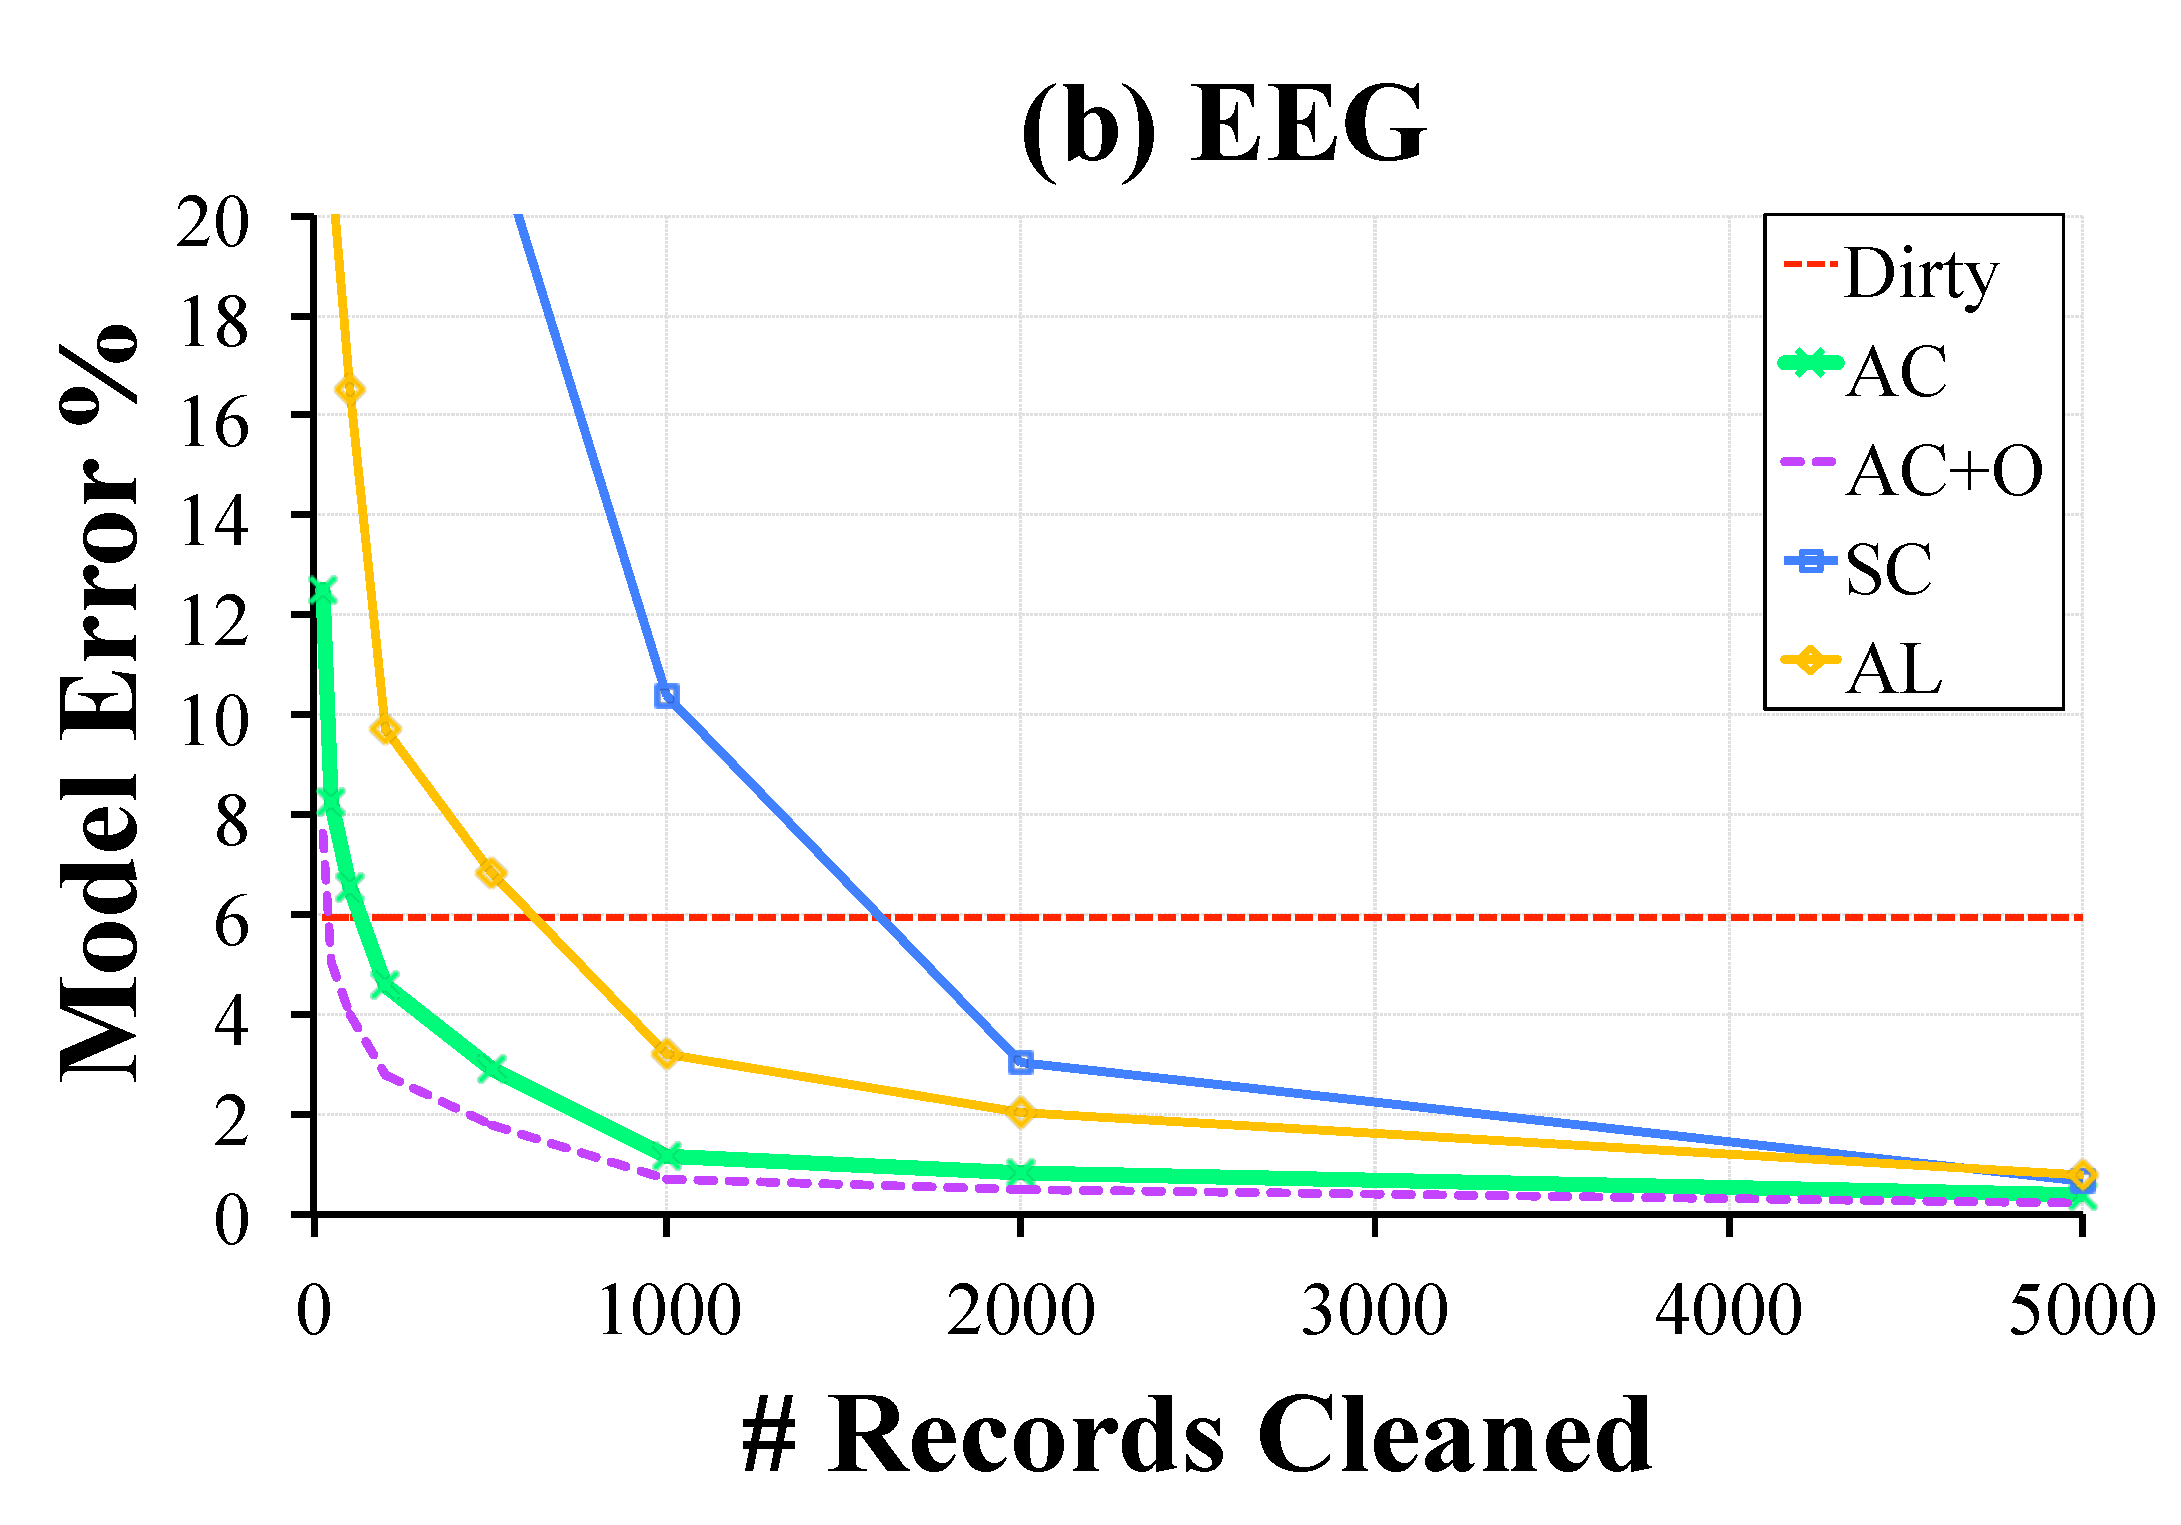
\includegraphics[width=0.49\columnwidth]{exp/exp3c.pdf}
  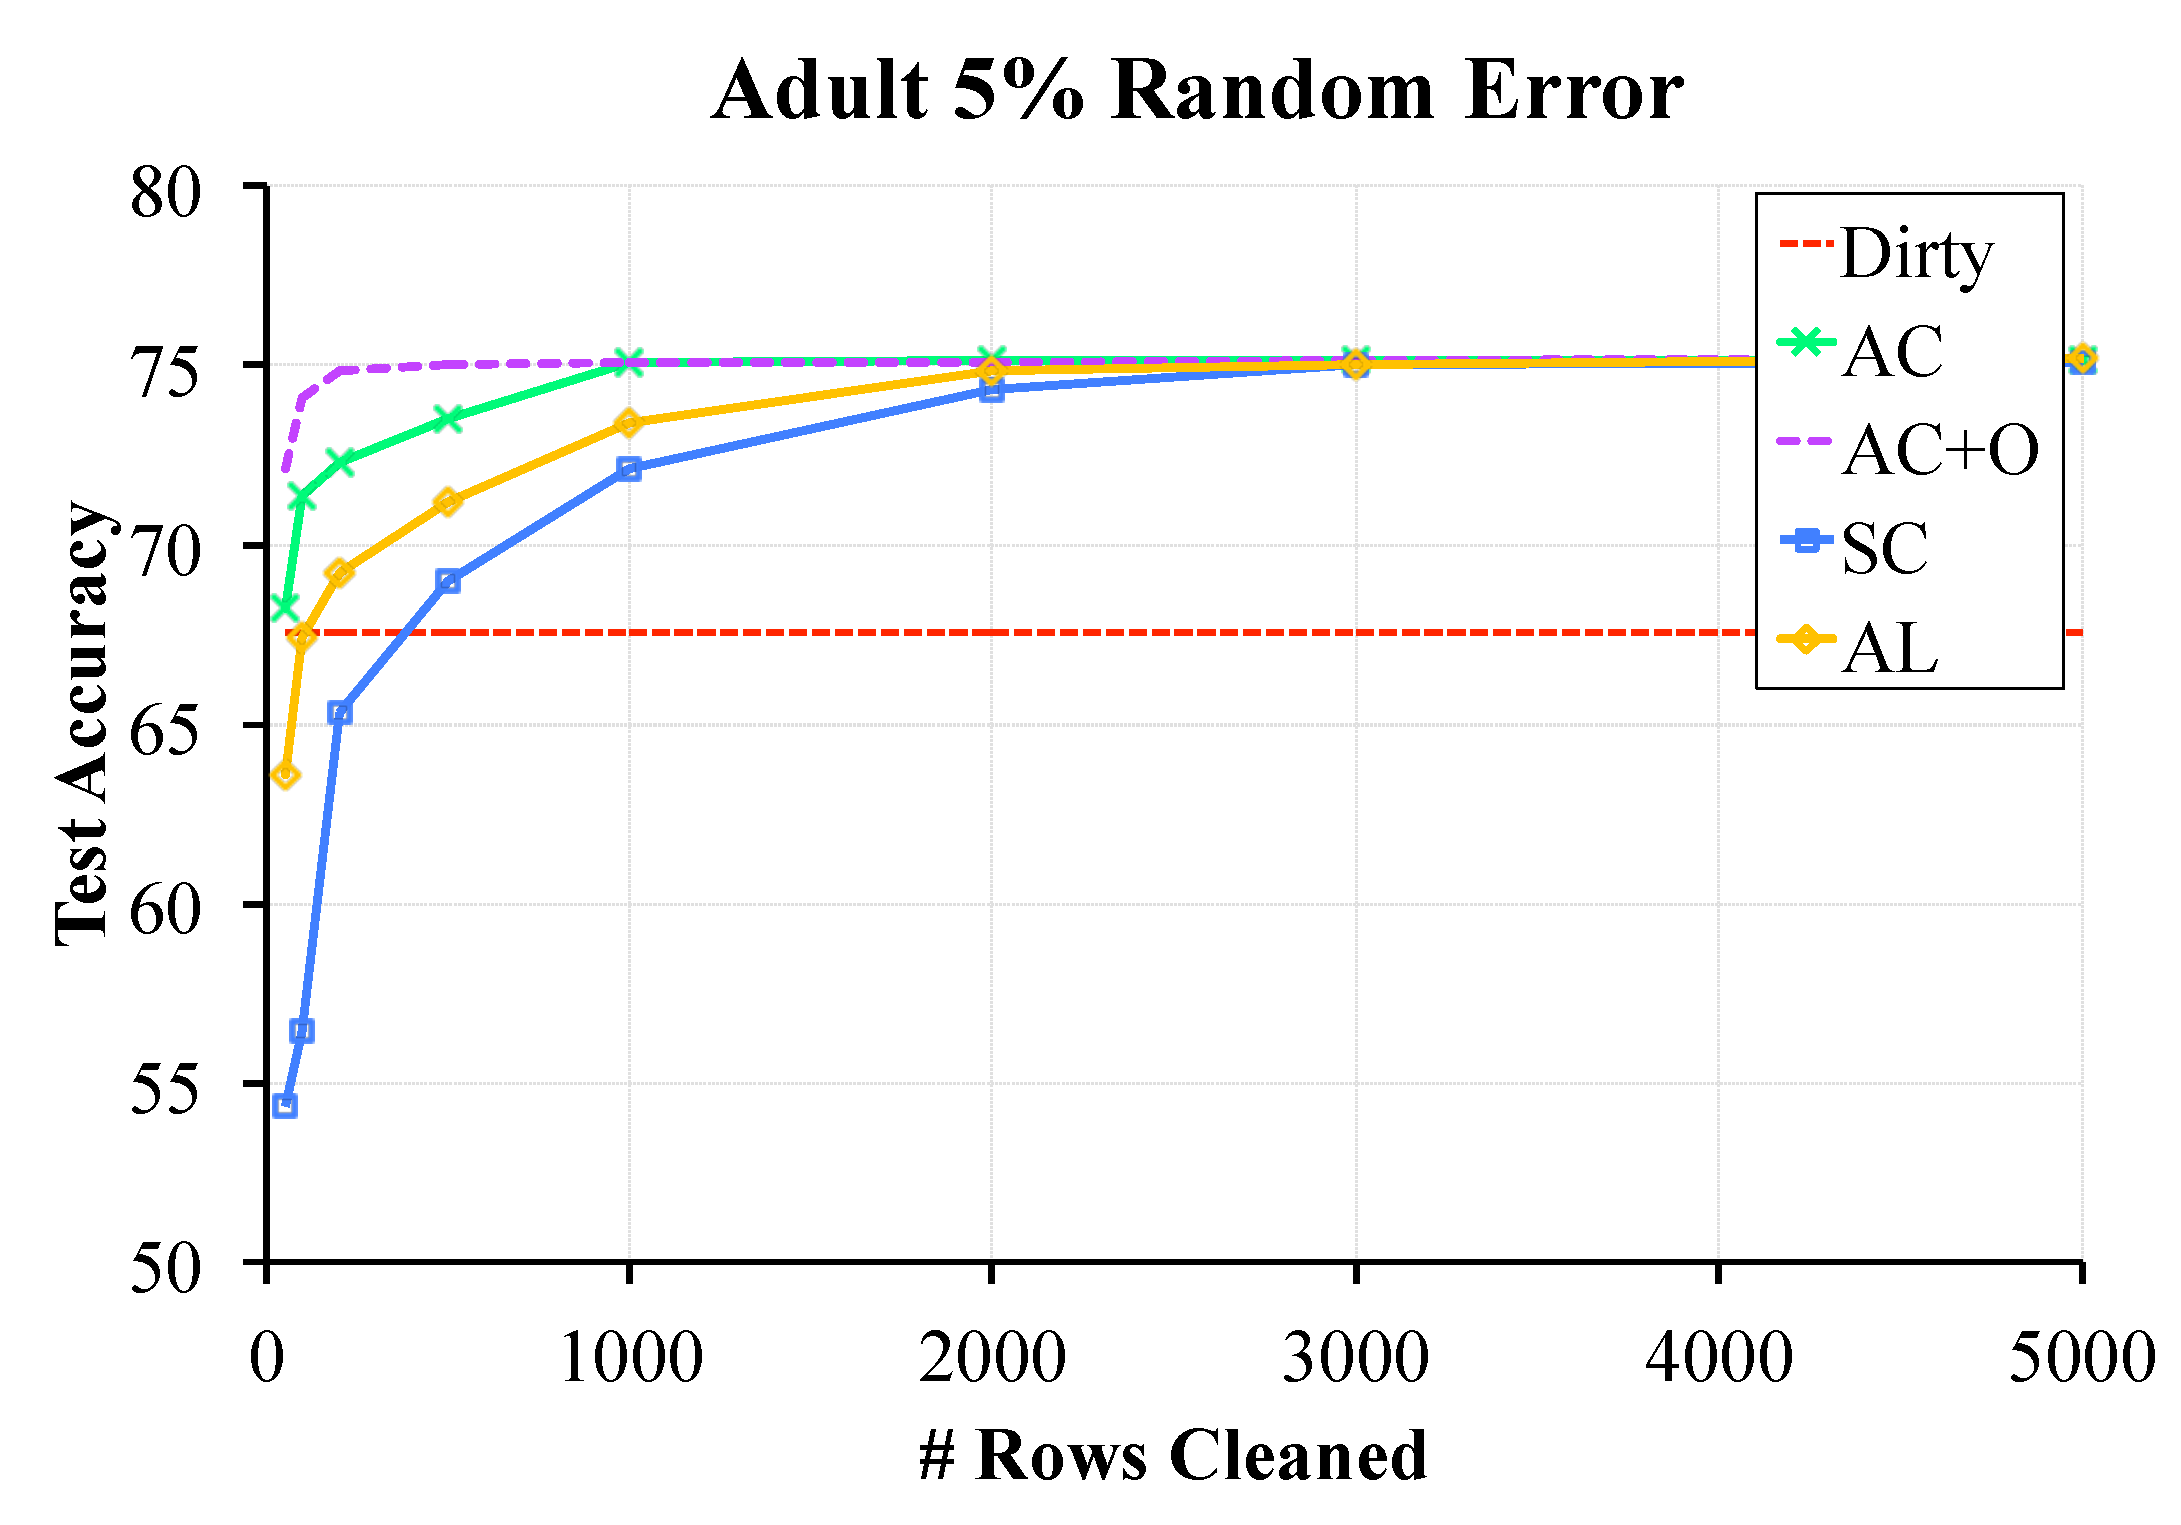
\includegraphics[width=0.49\columnwidth]{exp/exp3bb.pdf}
  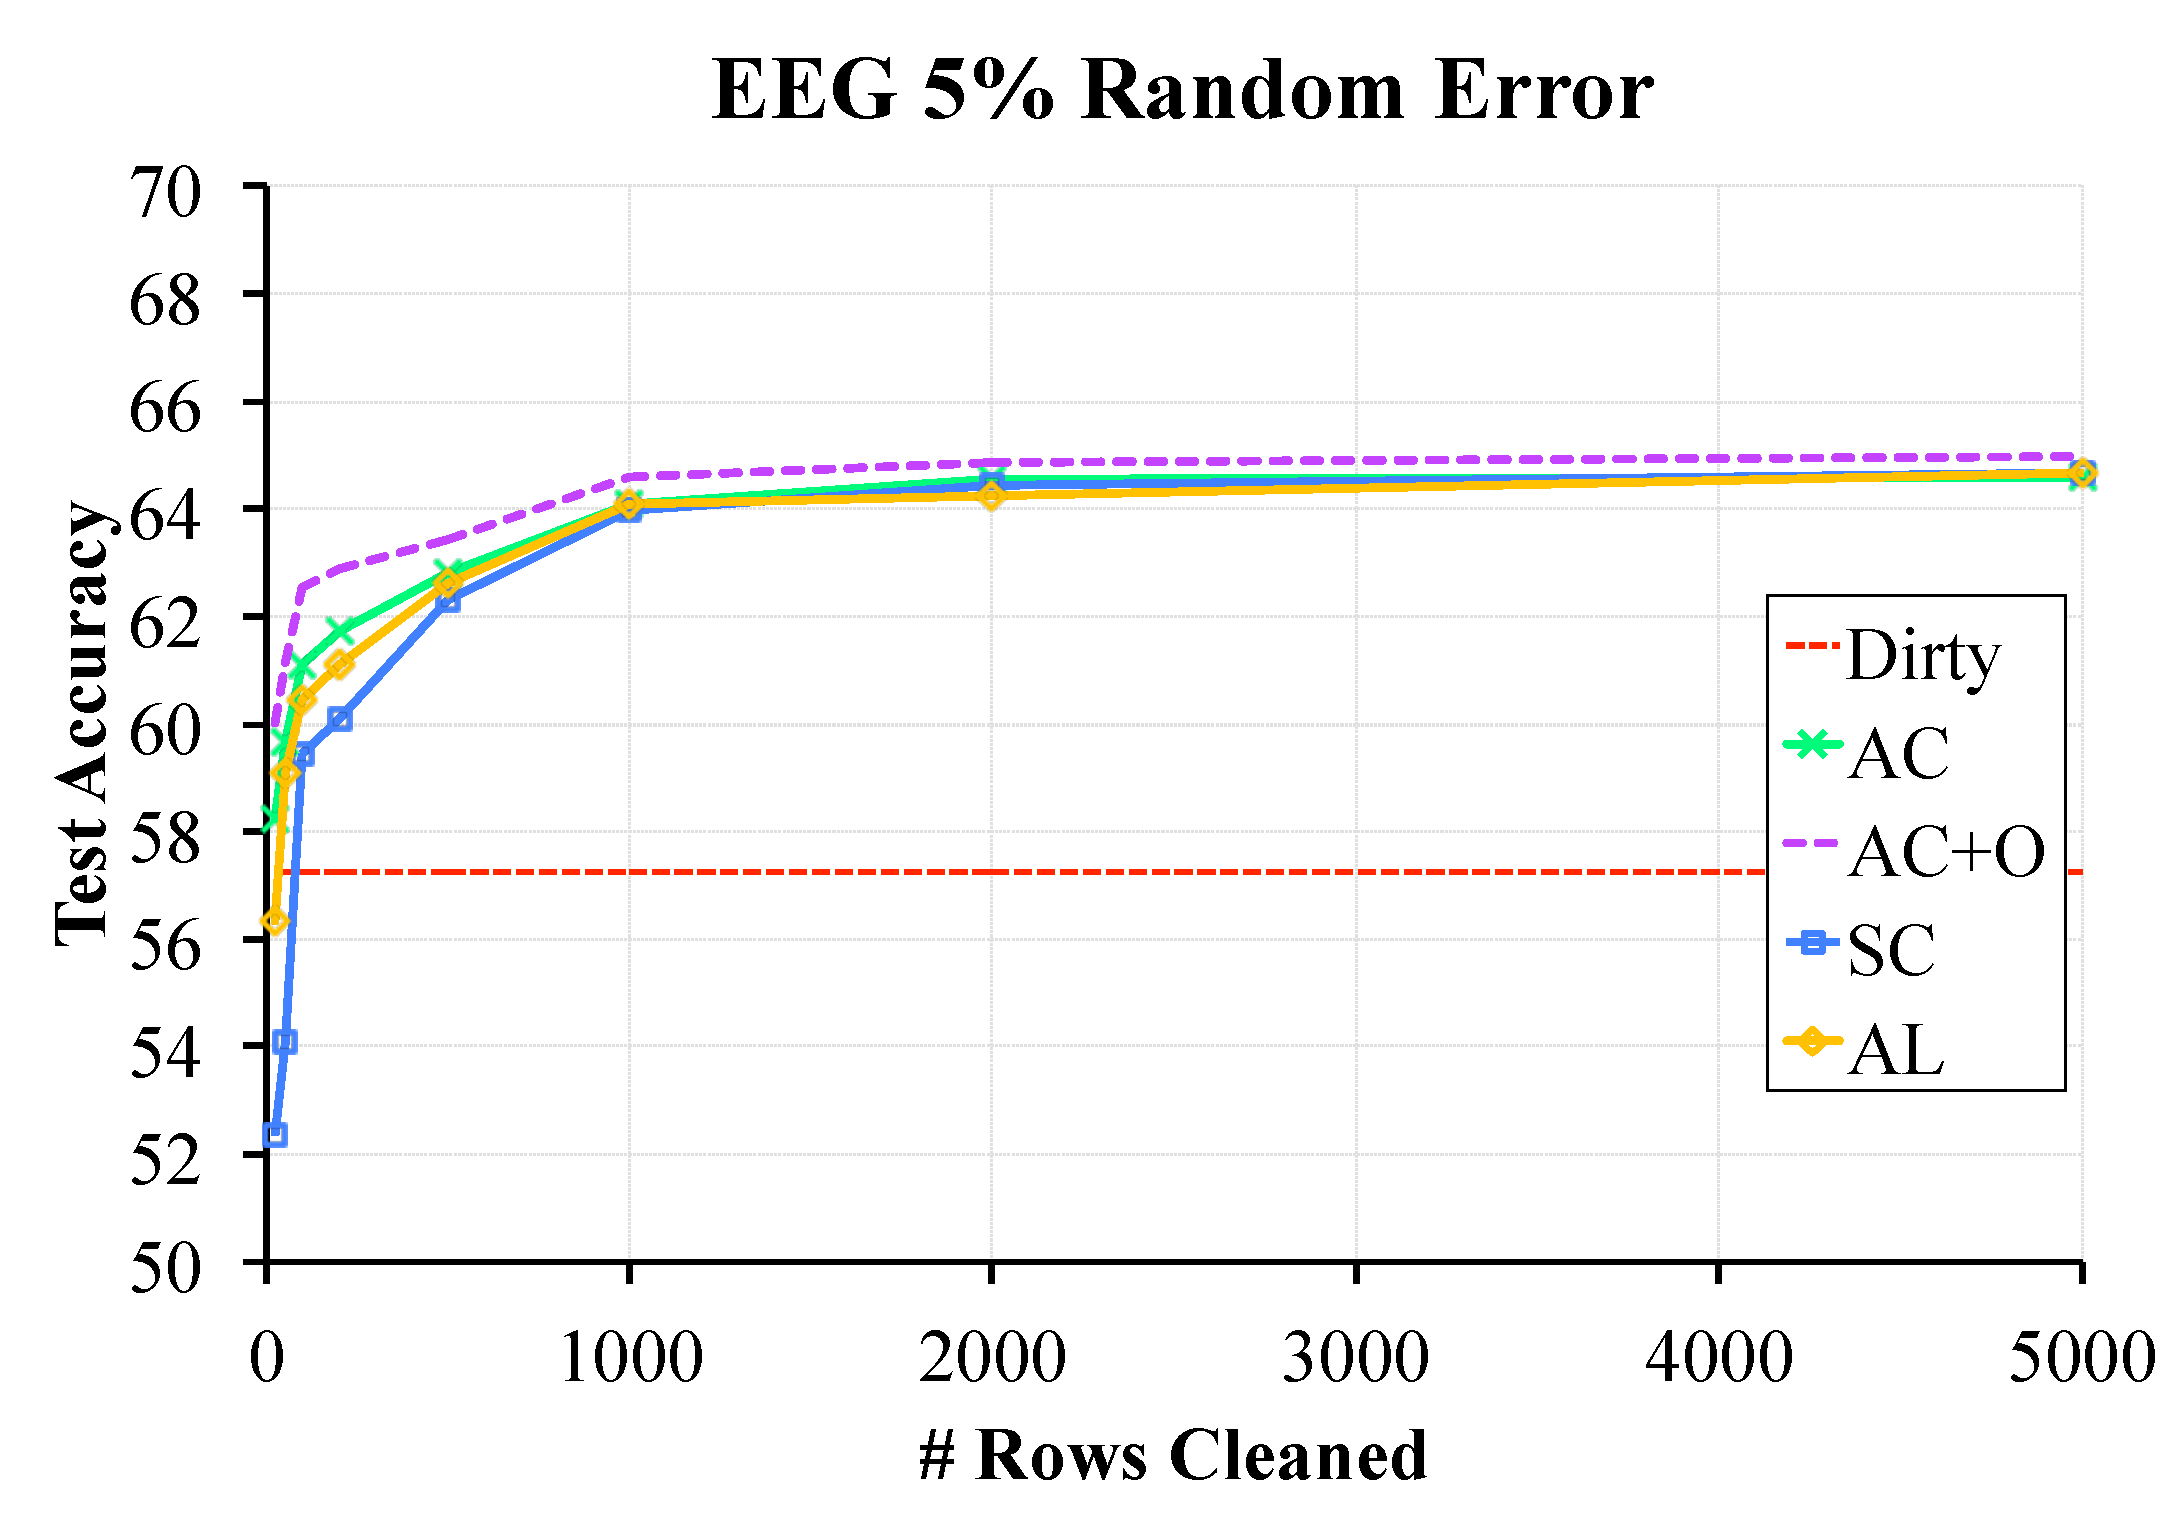
\includegraphics[width=0.49\columnwidth]{exp/exp3cc.pdf}
  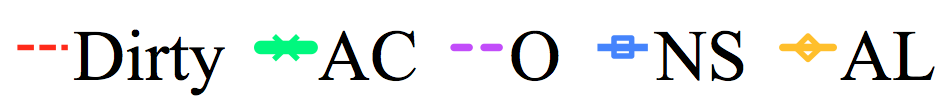
\includegraphics[width=0.5\columnwidth]{exp/legend-general.png}\vspace{-0.5em}
 \caption{ The relative model error as a function of the number of examples cleaned. \sys converges with a smaller sample size to the true result in comparison to Active Learning and SampleClean. \label{prio-perf}}\vspace{-1em}
\end{figure}

\subsubsection{Source of Improvements}
The next experiment compares the performance of \sys with and without various optimizations at 500 records cleaned point. 
This is a vertical slice of the plots in the previous experiments.
\sys without detection is denoted as (AC-D) (that is at each iteration we sample from the entire dirty data), and \sys without detection and importance sampling is denoted as (AC-D-I).
Figure \ref{opts} plots the relative error of the alternatives and \sys with and without the optimizations.
Without detection (AC-D), \sys is still more accurate than Active Learning.
Removing the importance sampling, \sys is slightly worse than Active Learning on the Adult dataset but is comparable on the EEG dataset.

\vspace{0.25em}

\noindent \emph{Summary: Both a priori detection and non-uniform sampling significantly contribute to the gains over Active Learning.}

\begin{figure}[ht!]
\centering
 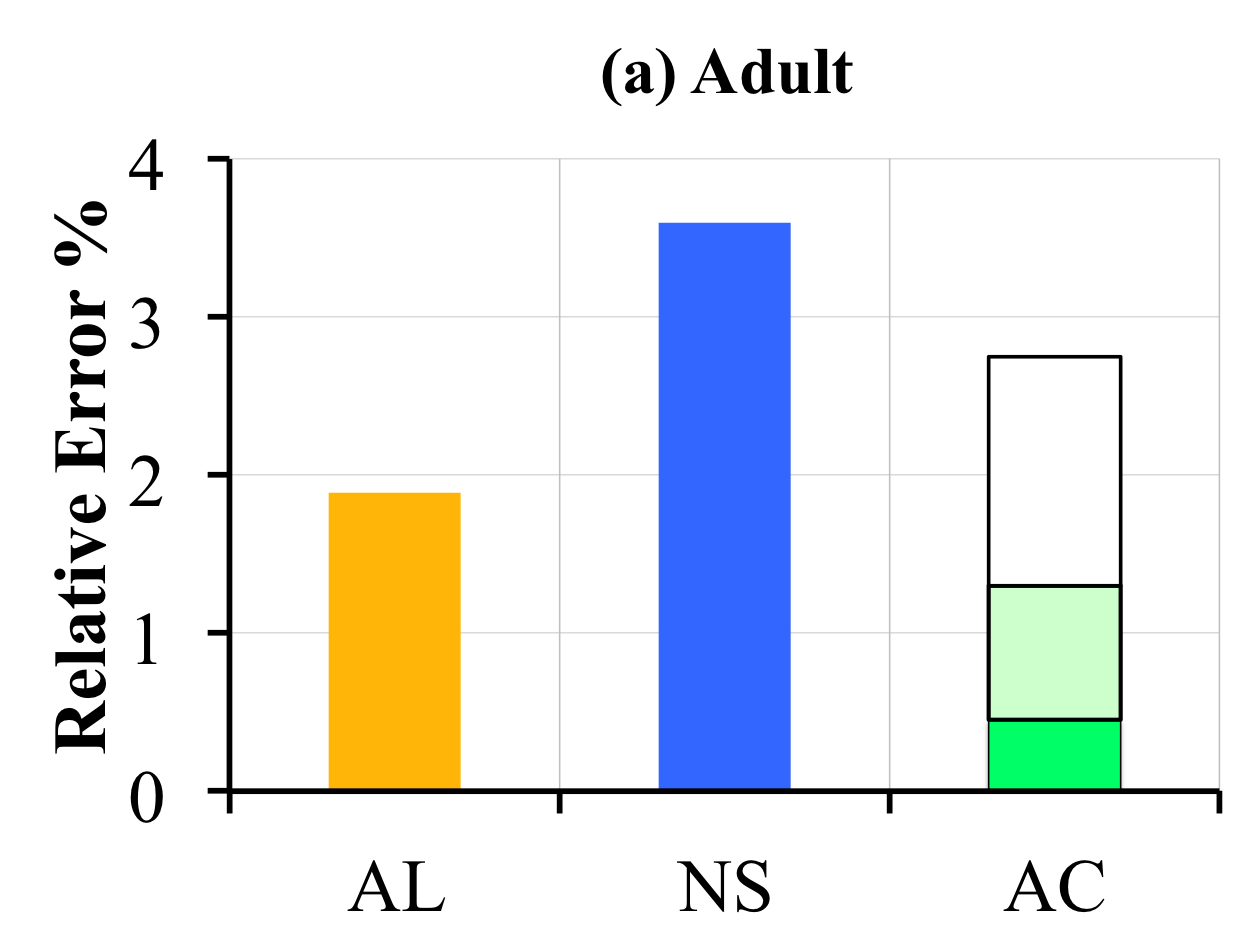
\includegraphics[width=0.49\columnwidth]{exp/exp8a.png}
 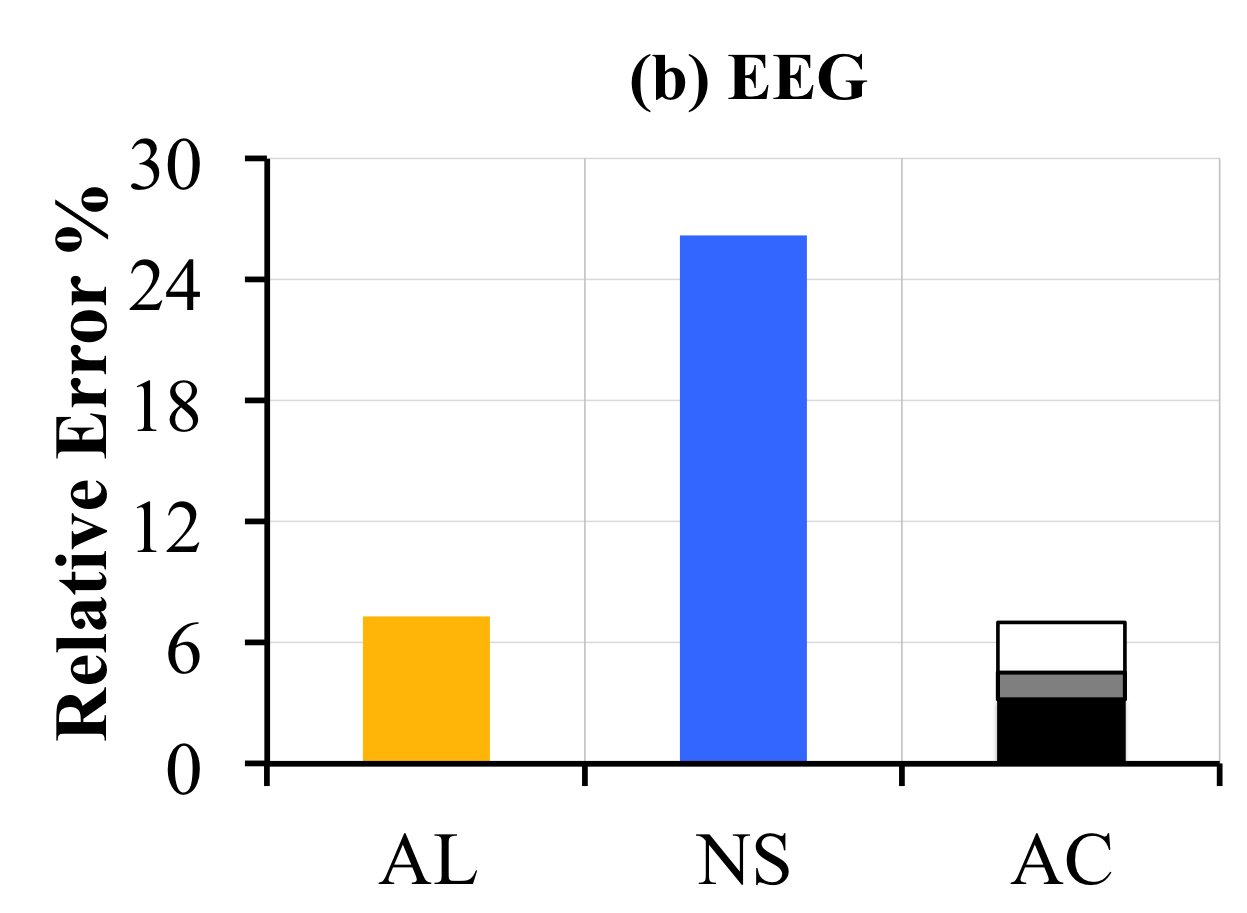
\includegraphics[width=0.49\columnwidth]{exp/exp8b.png}
 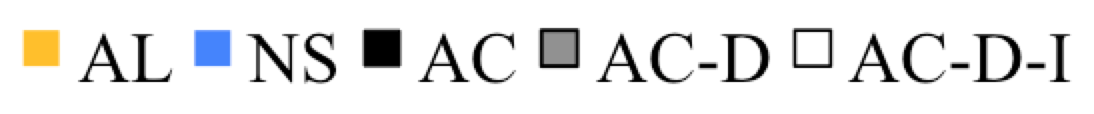
\includegraphics[width=0.5\columnwidth]{exp/legend-8.png}\vspace{-1em}
 \caption{ -D denotes no detection, and -D-I denotes no detection and no importance sampling. Both optimizations significantly help \sys outperform SampleClean and Active Learning. \label{opts}}\vspace{-1.5em}
\end{figure}

\iffalse
We evaluate Active Learning and \sys to better understand this relationship.
In Figure \ref{albias}, we vary the biasing effect of the random corruptions.
That is, we start with zero mean noise and increase the mean value and variance of the noise.
Since Active Learning uses the gradient, if there is zero mean noise, in expectation, the dirty data and clean data are the same.
However, as the bias increases, the fact that Active Learning prioritizes w.r.t to the dirty data matters more and becomes increasingly erroneous w.r.t to \sys.

\begin{figure}[ht!]
\centering
 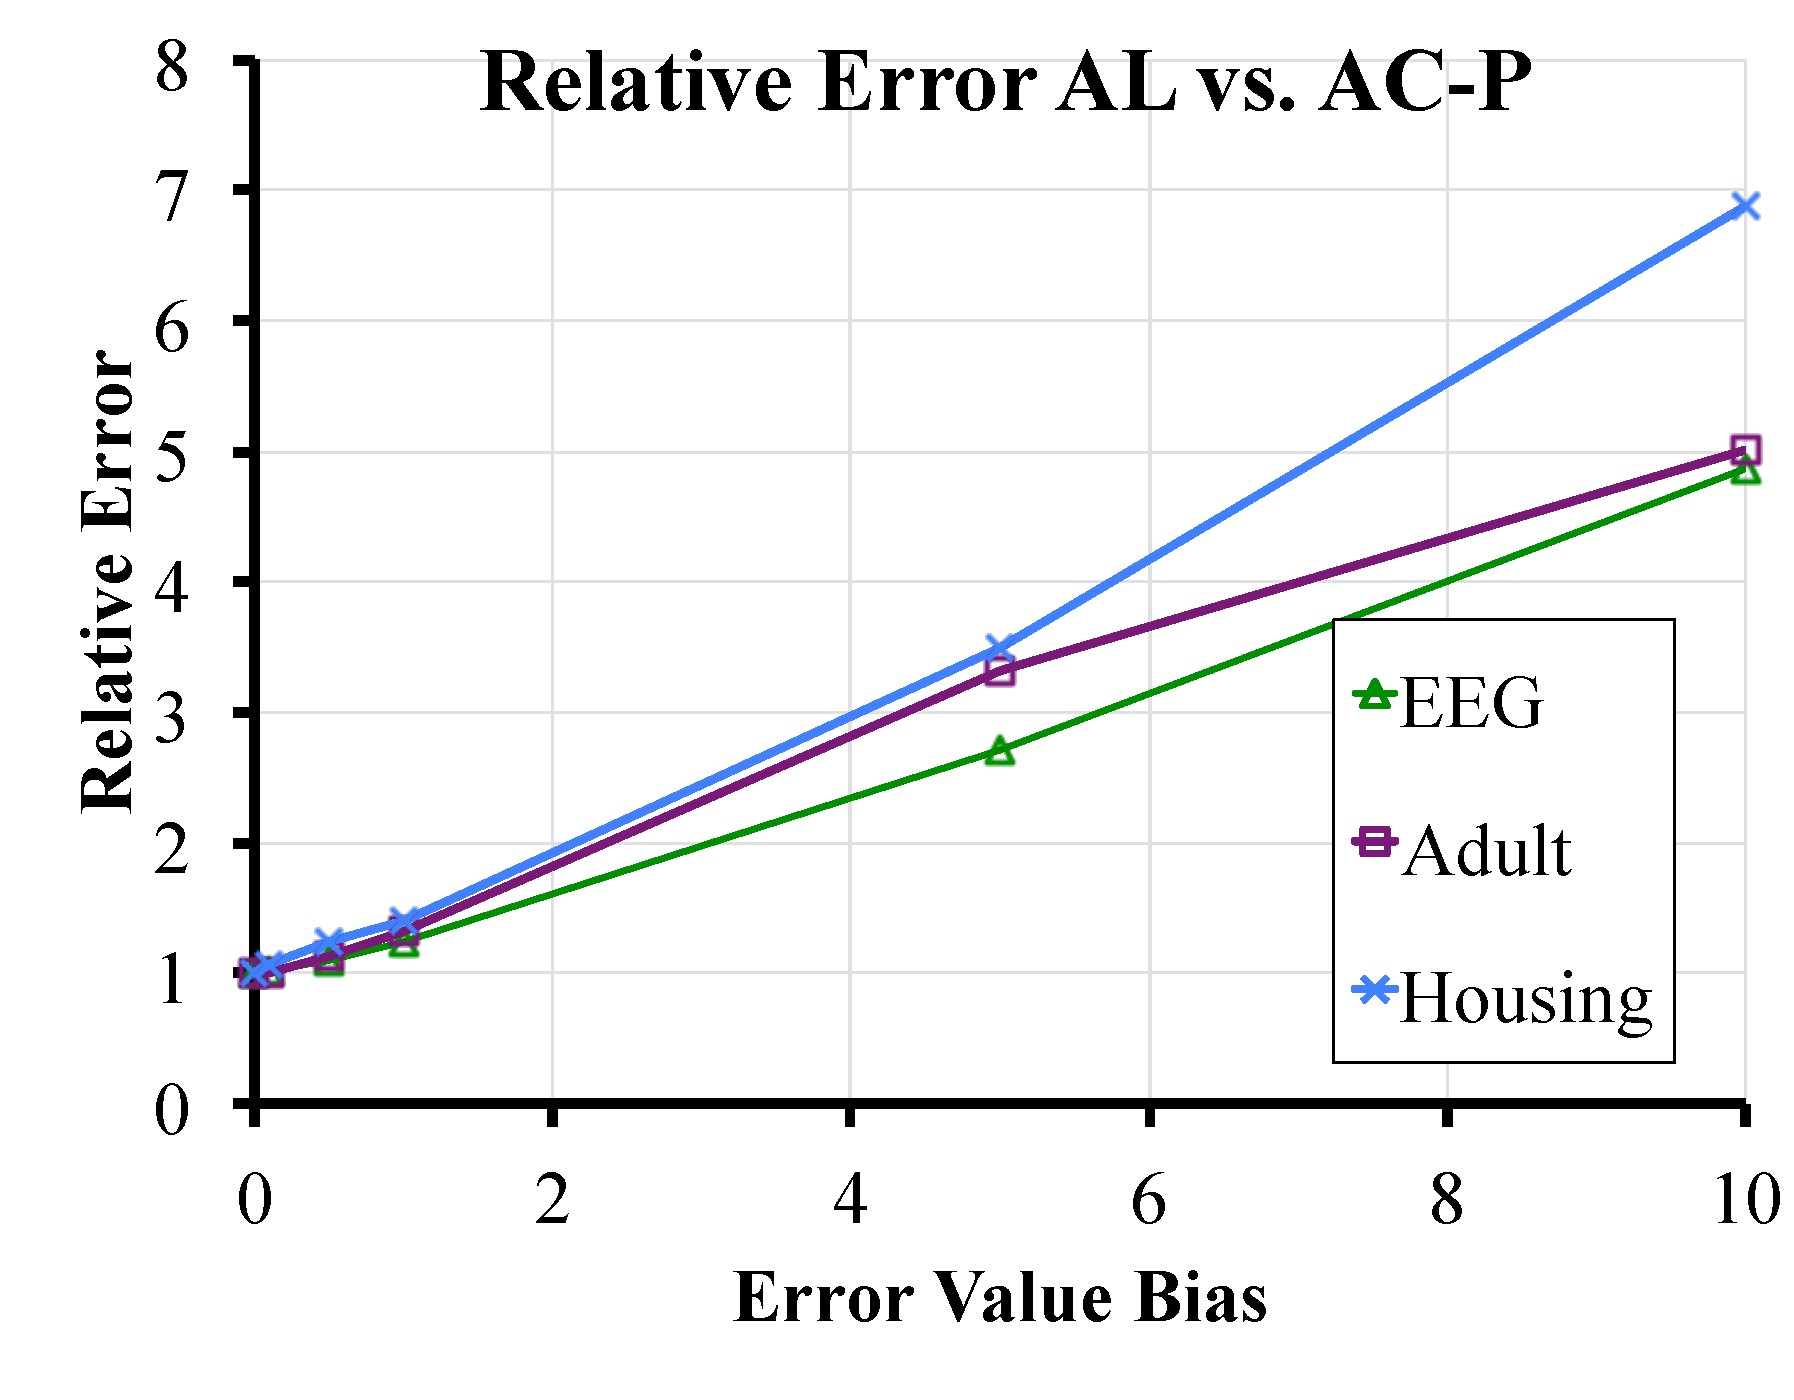
\includegraphics[width=0.6\columnwidth]{exp/exp10.pdf}
 \caption{As we increase the biasing nature of the corruption, Active Learning is increasingly erroneous w.r.t \sys. \label{albias}}
\end{figure}
\fi

\subsubsection{Mixing Dirty and Clean Data}
Training a model on mixed data is an unreliable methodology lacking the same guarantees as Active Learning or SampleClean even in the simplest of cases.
For thoroughness, the next experiments include the model error as a function of records cleaned in comparison to \sys.
Figure \ref{pc-perf} plots the same curves as the previous experiment comparing \sys, Active Learning, and two mixed data algorithms.
PC randomly samples data, clean, and writes-back the cleaned data.
PC+D randomly samples data from using the dirty data detector, cleans, and writes-back the cleaned data.
For these errors PC and PC+D give reasonable results (not always guaranteed), but \sys converges faster.
This is because \sys tunes the weighting when averaging dirty and clean data into the gradient.

\begin{figure}[ht!]
\centering
 %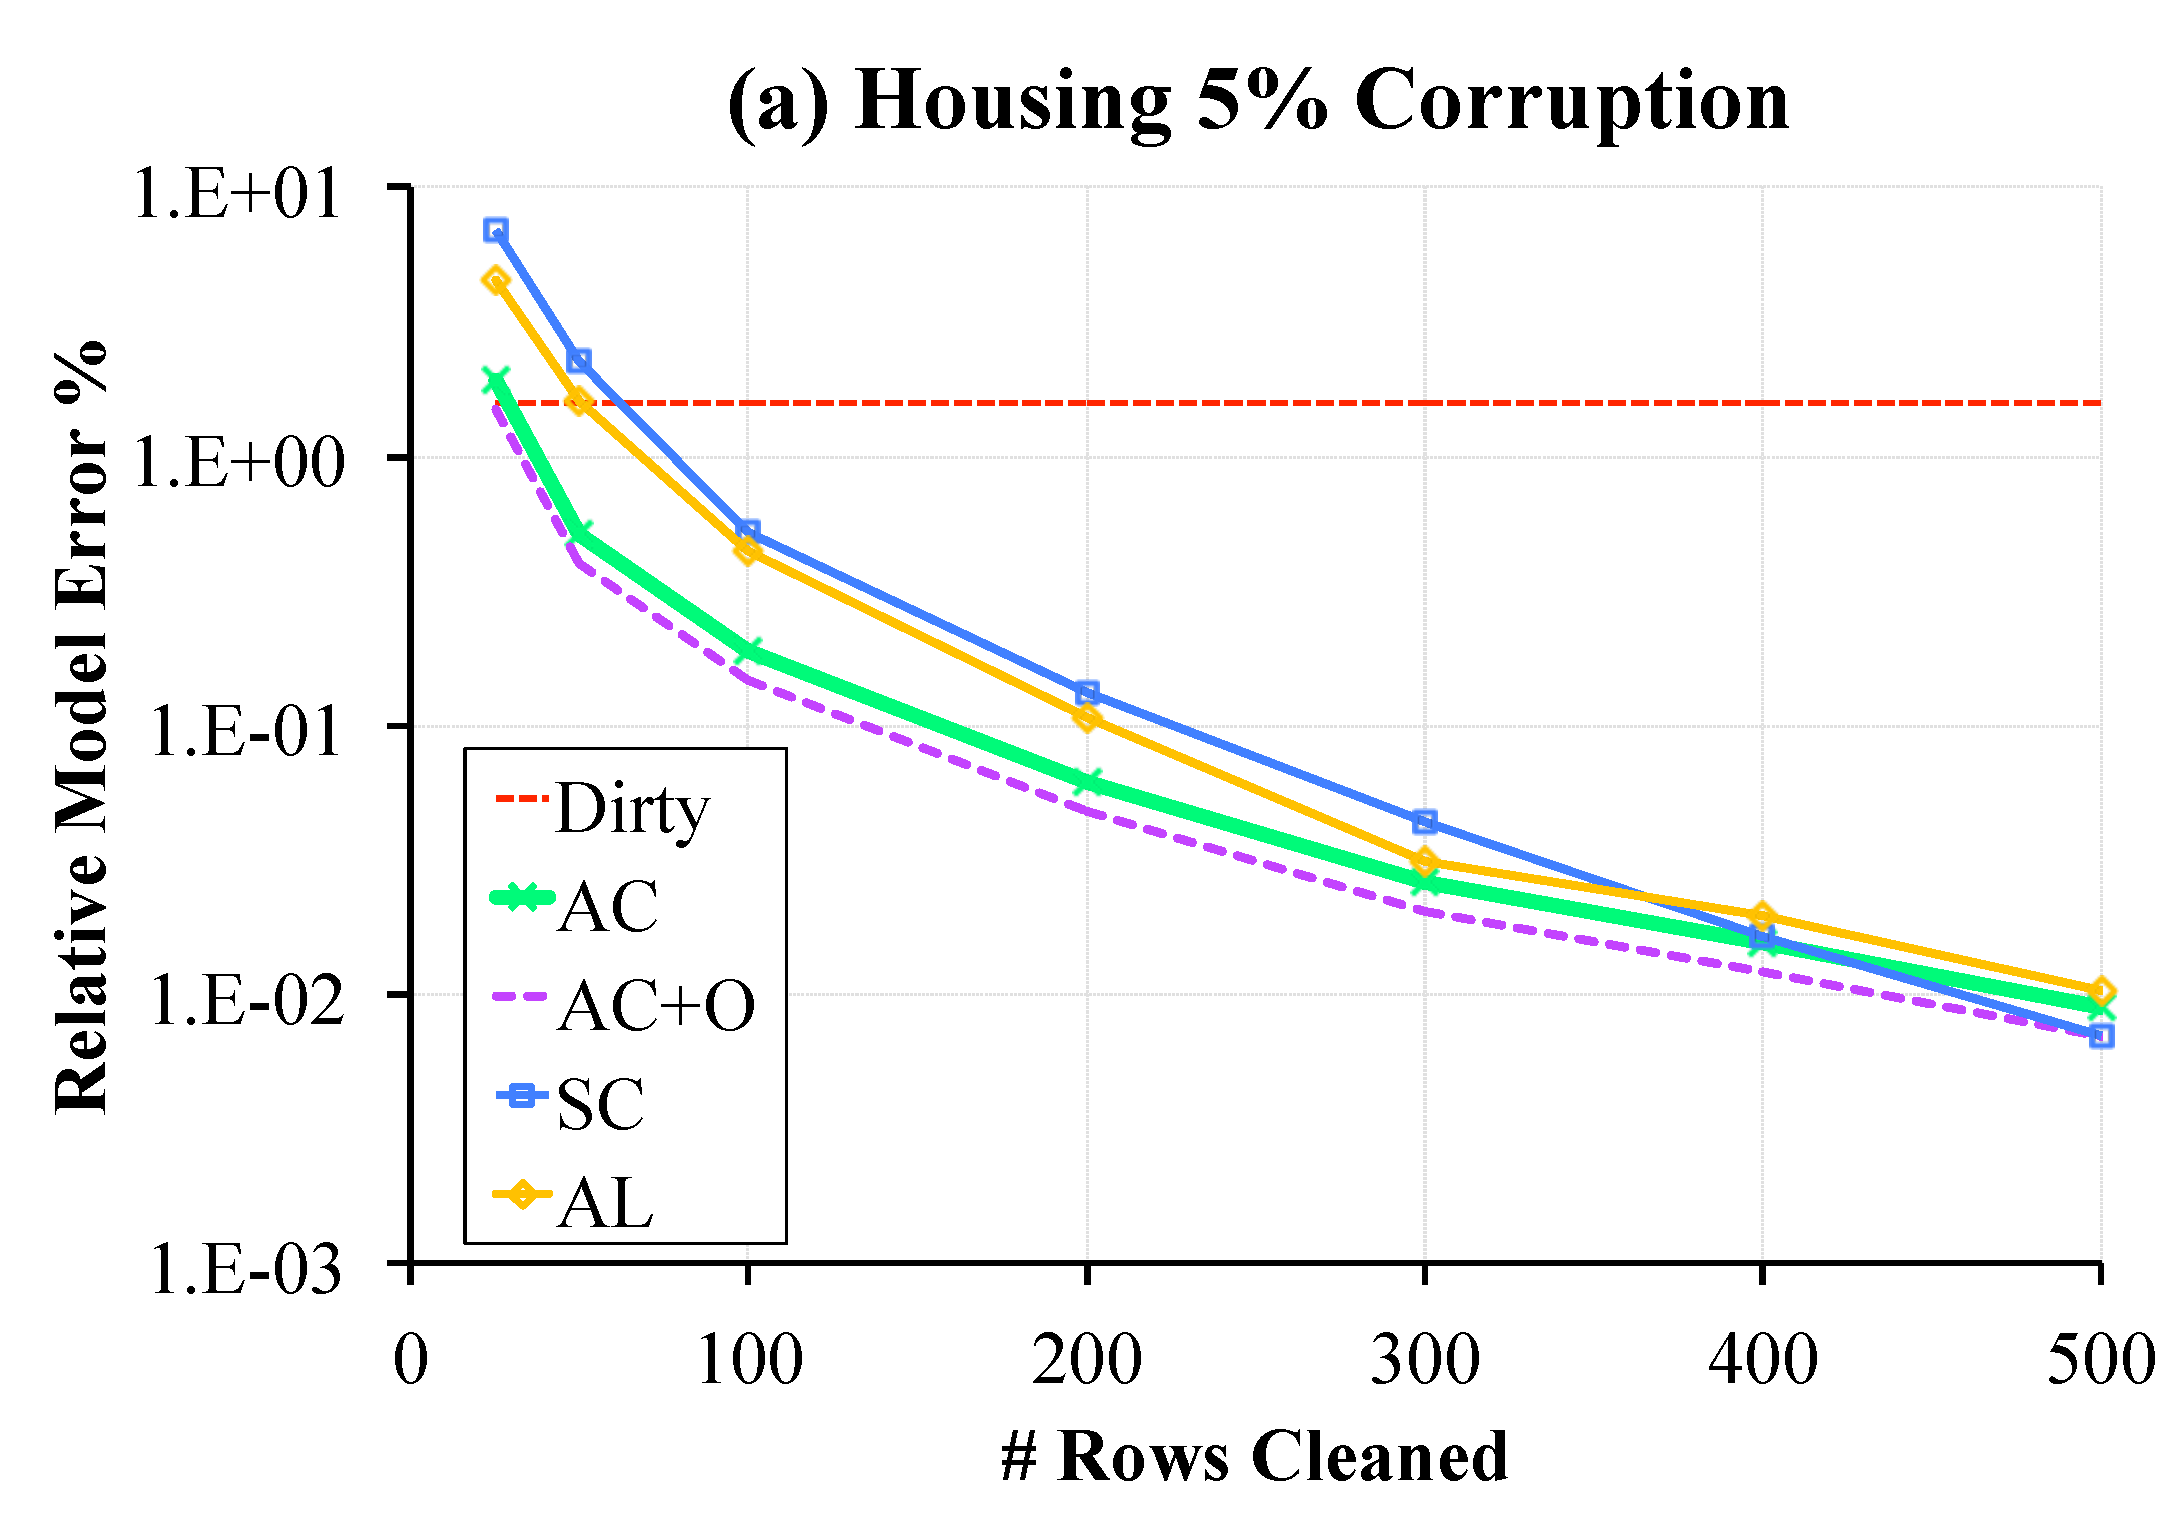
\includegraphics[scale=0.15]{exp/exp3a.pdf}
 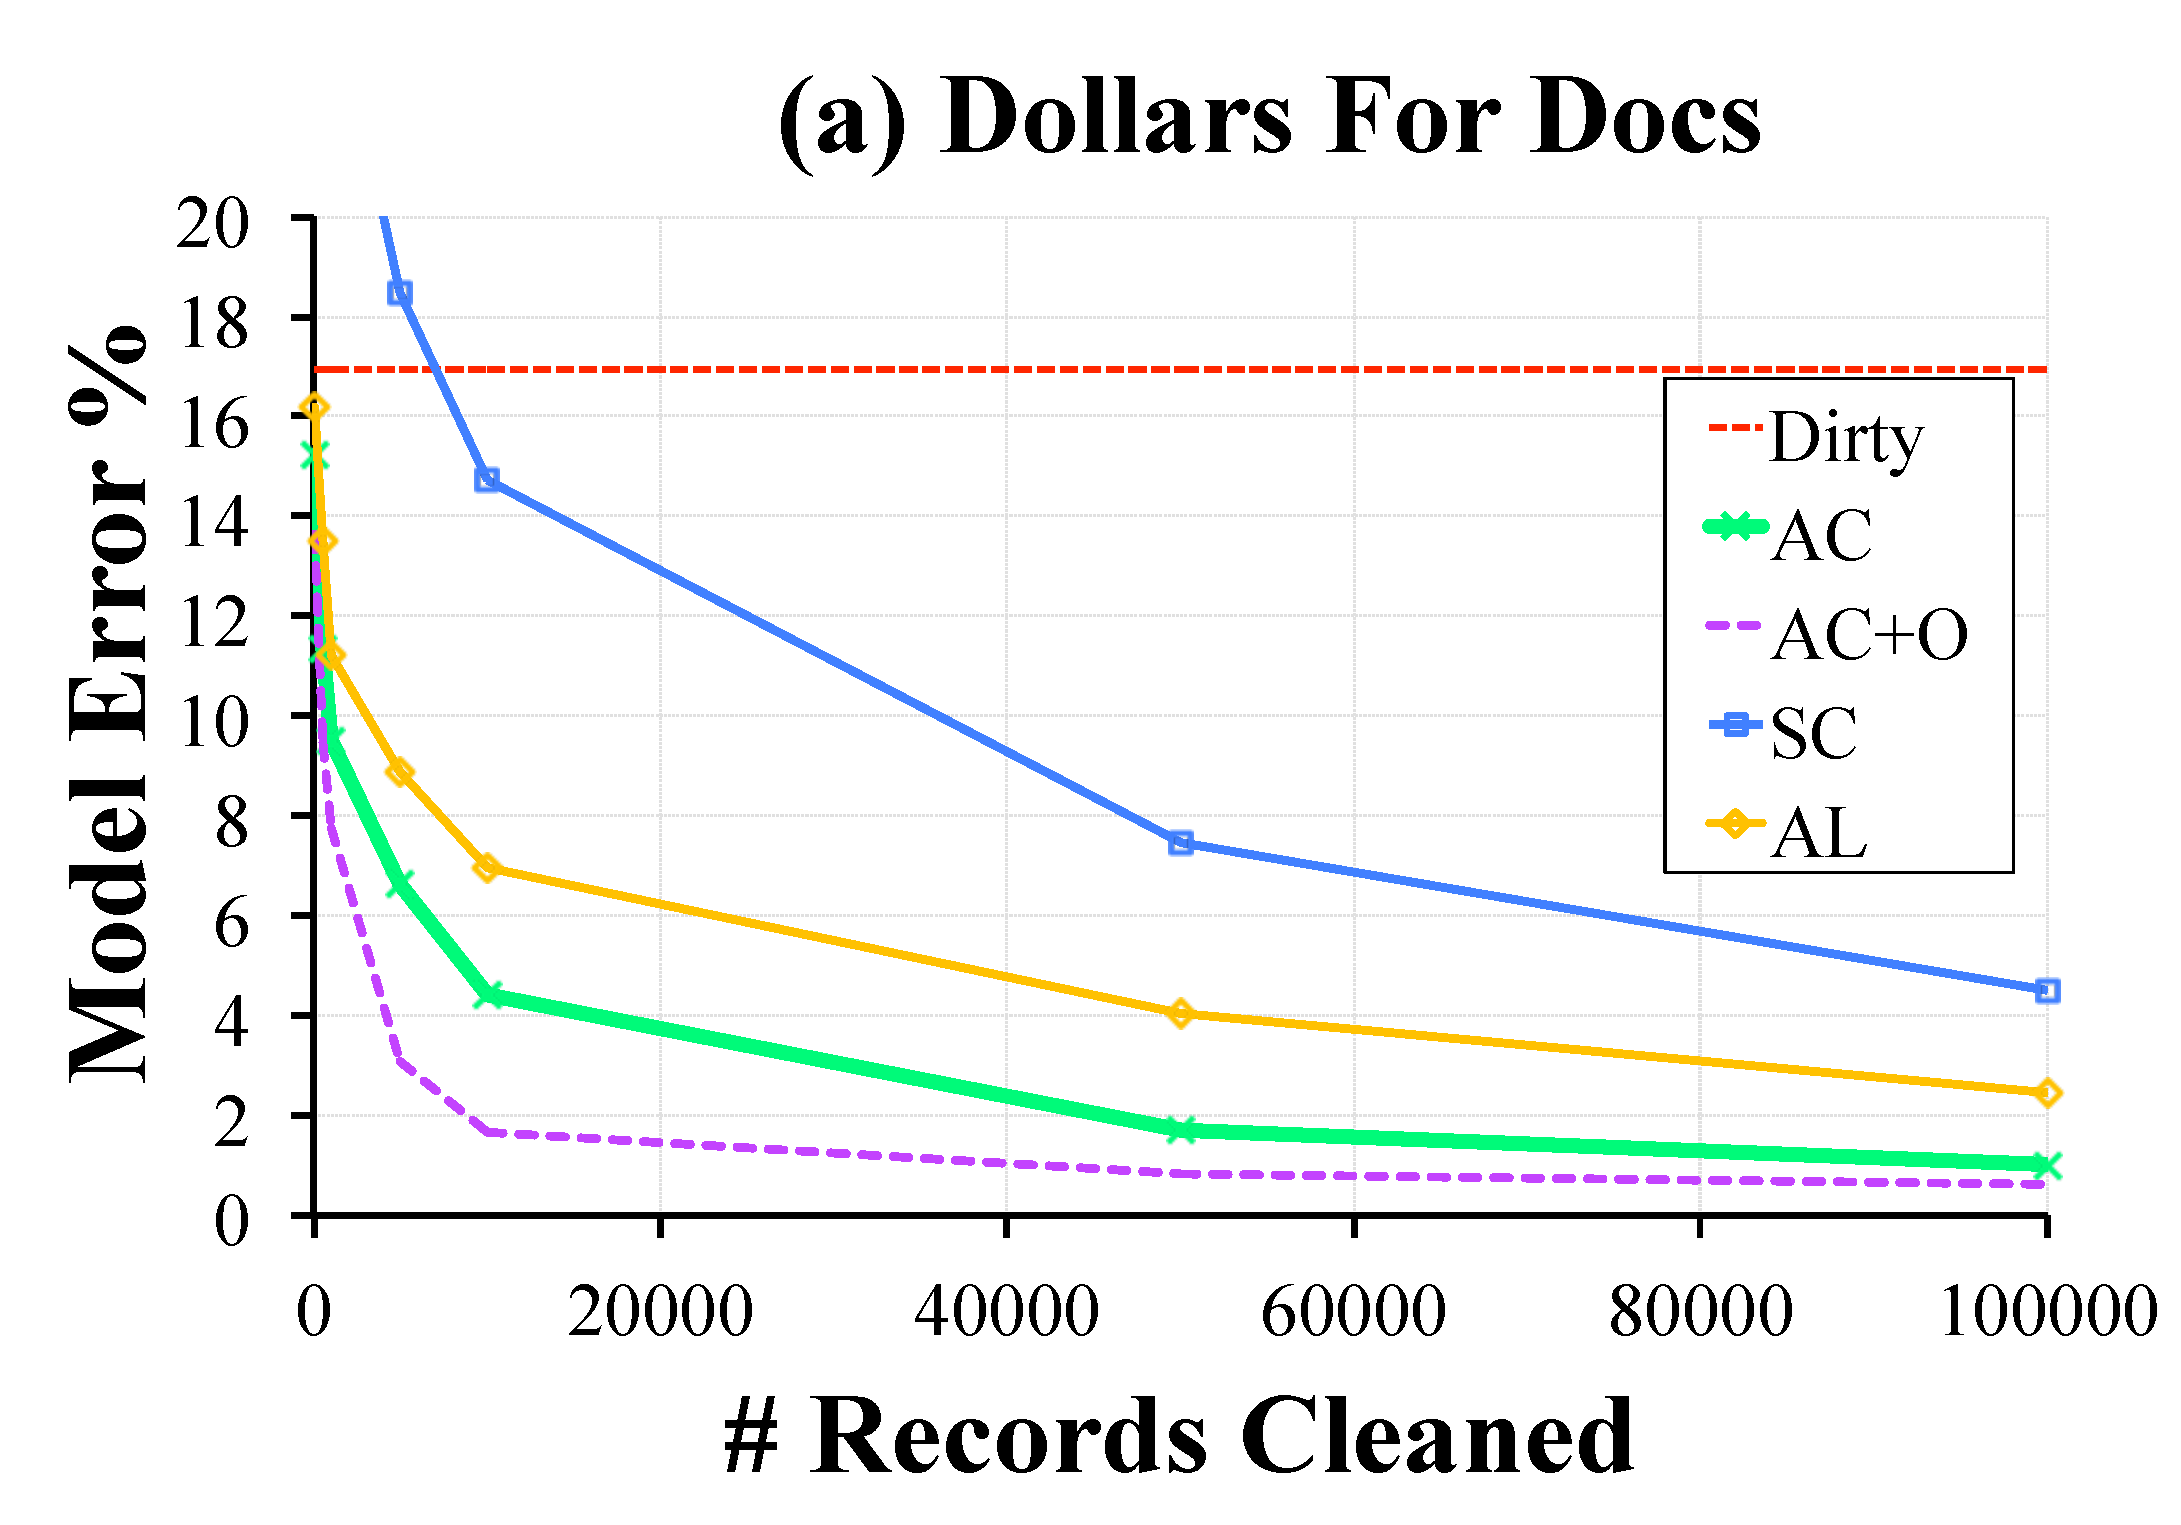
\includegraphics[width=0.49\columnwidth]{exp/exp14a.pdf}
    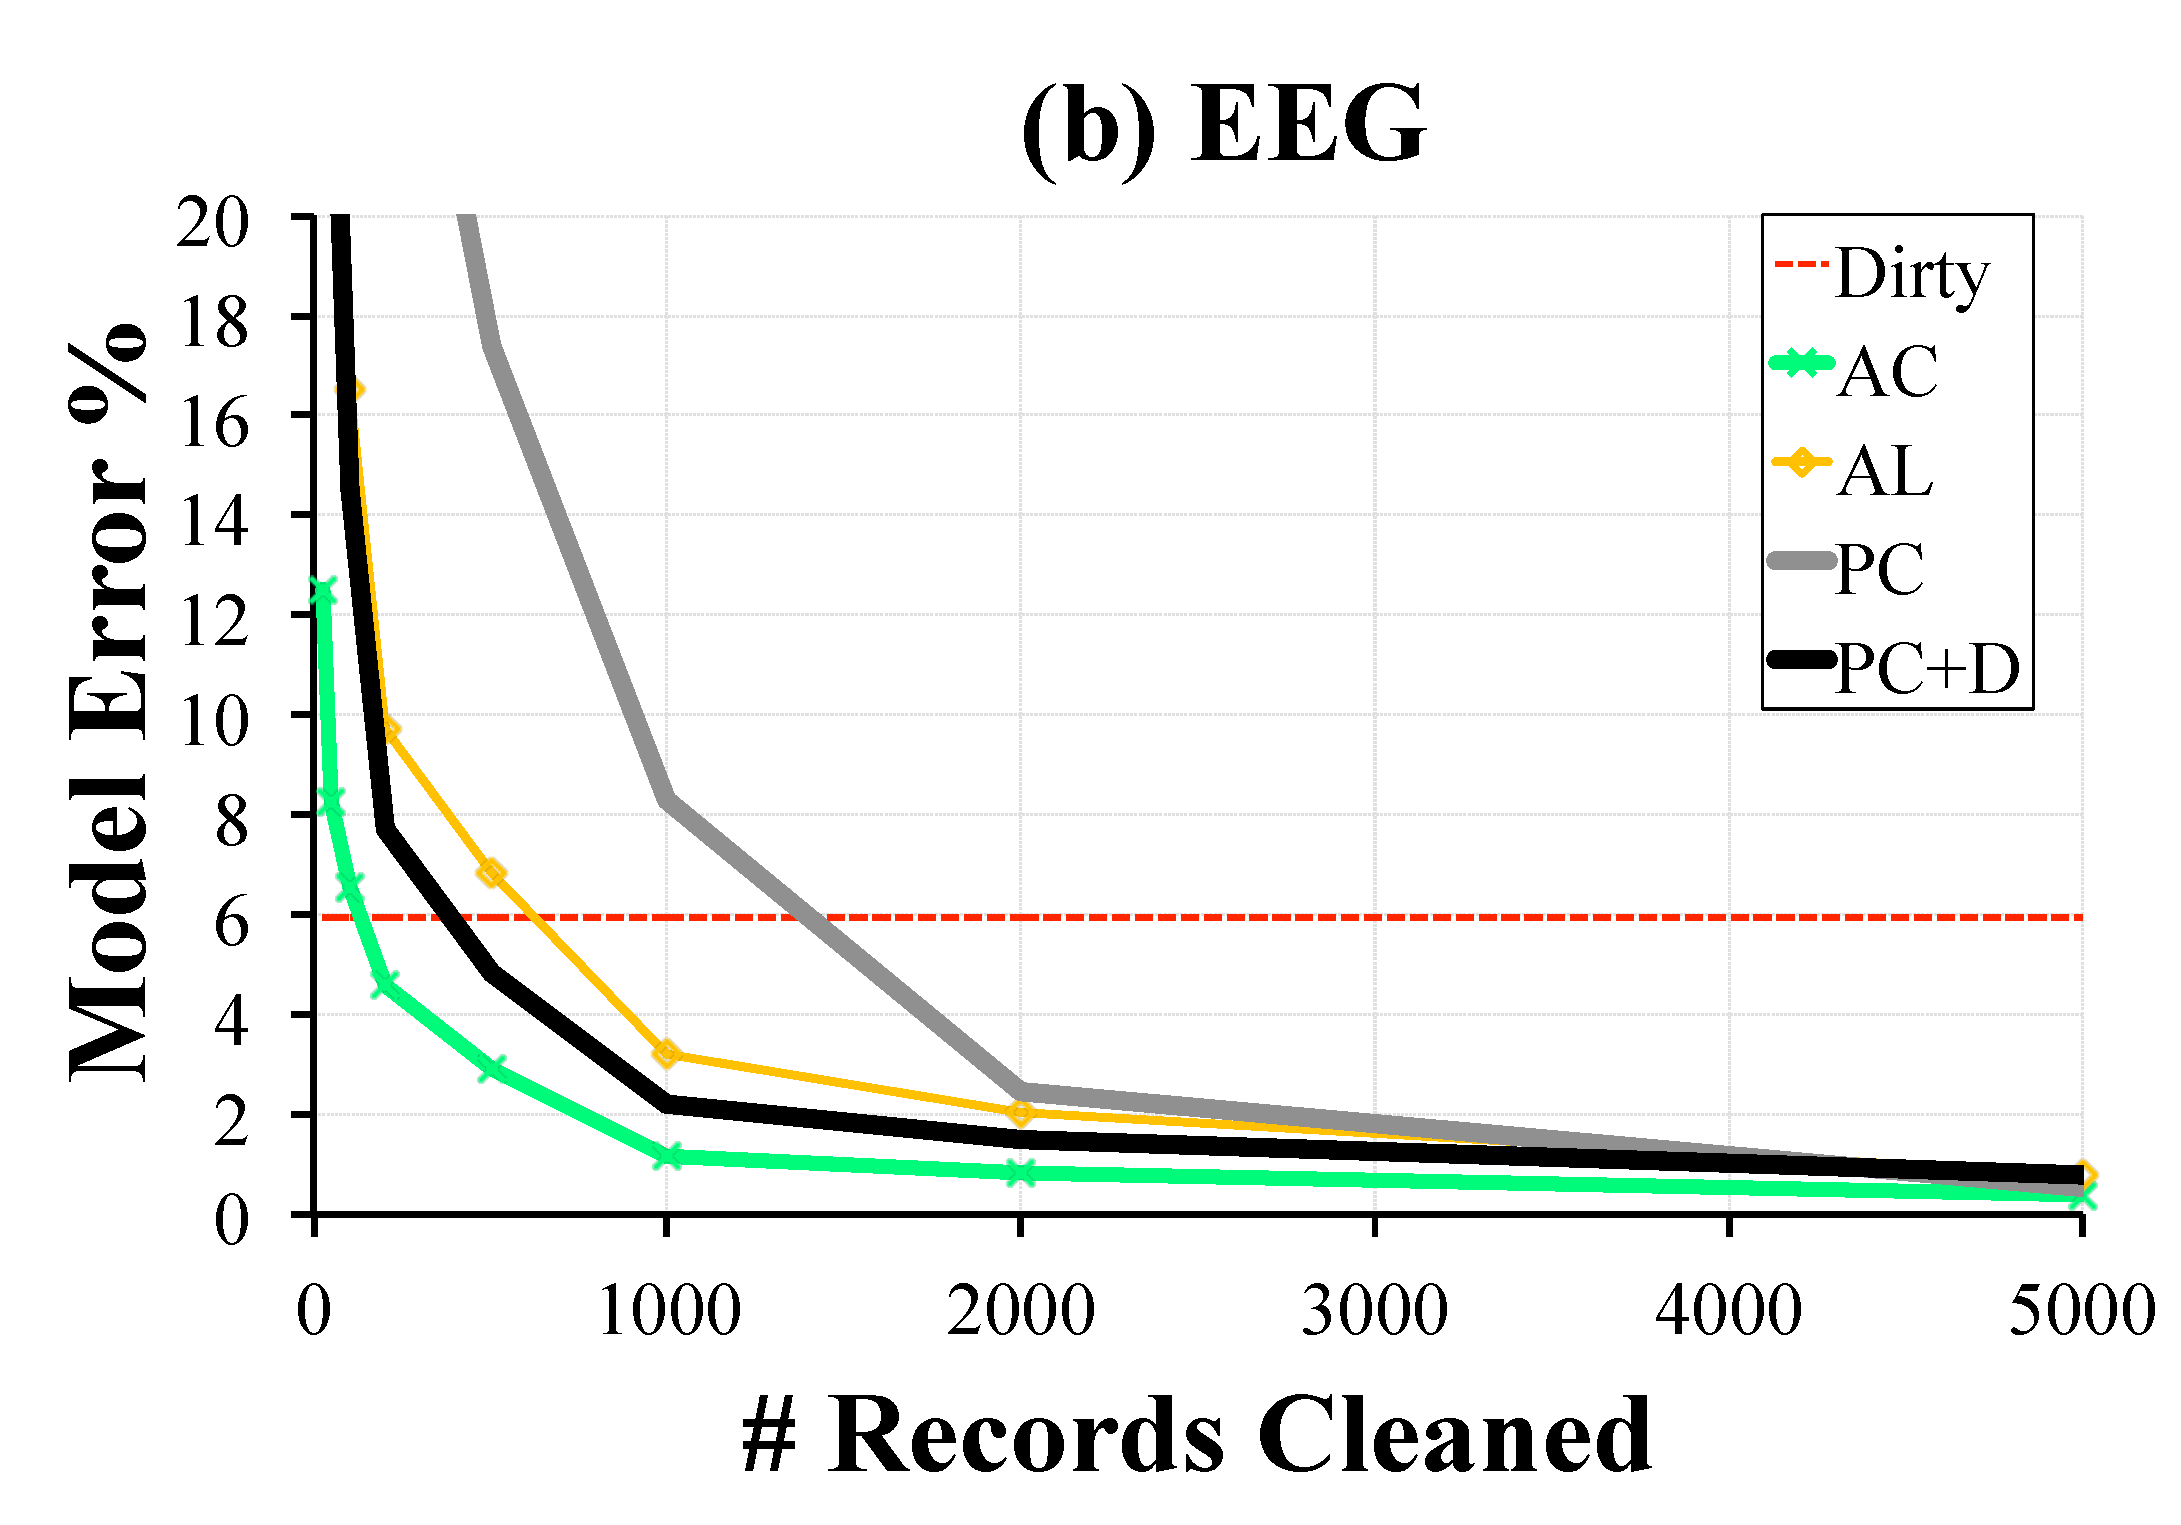
\includegraphics[width=0.49\columnwidth]{exp/exp14b.pdf}
    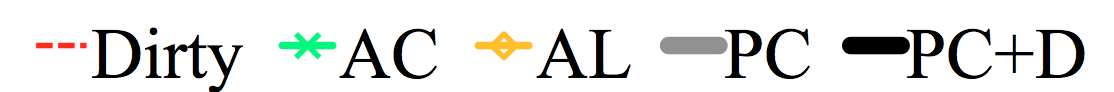
\includegraphics[width=0.49\columnwidth]{exp/legend-14.png}\vspace{-0.5em}
 \caption{The relative model error as a function of the number of examples cleaned. \sys converges with a smaller sample size to the true result in comparison to partial cleaning (PC,PC+D).  \label{pc-perf}}
\end{figure}

\noindent \emph{Summary: \sys converges faster than mixing dirty and clean data since it reweights data based on the fraction that is dirty and clean. Partial cleaning is not guaranteed to give sensible results.}

\subsubsection{Corruption Rate}
The next experiment explores how much of the performance
is due to the initialization with the dirty model (i.e., SampleClean trains a model from ``scratch").
Figure \ref{bias} varies the systematic corruption rate and plots the number of records cleaned to achieve 1\% relative error for SampleClean and \sys.
SampleClean does not use the dirty data and thus its error is essentially governed by the Central Limit Theorem.
SampleClean outperforms \sys only when corruptions are very severe (45\% in Adult and nearly 60\% in EEG).
When the initialization with the dirty model is inaccurate, \sys does not perform as well. 

\vspace{0.25em}

\noindent \emph{Summary: SampleClean is beneficial in comparison to \sys when corruption rates exceed 45\%.}

\begin{figure}[ht!]
\centering\vspace{-1em}
 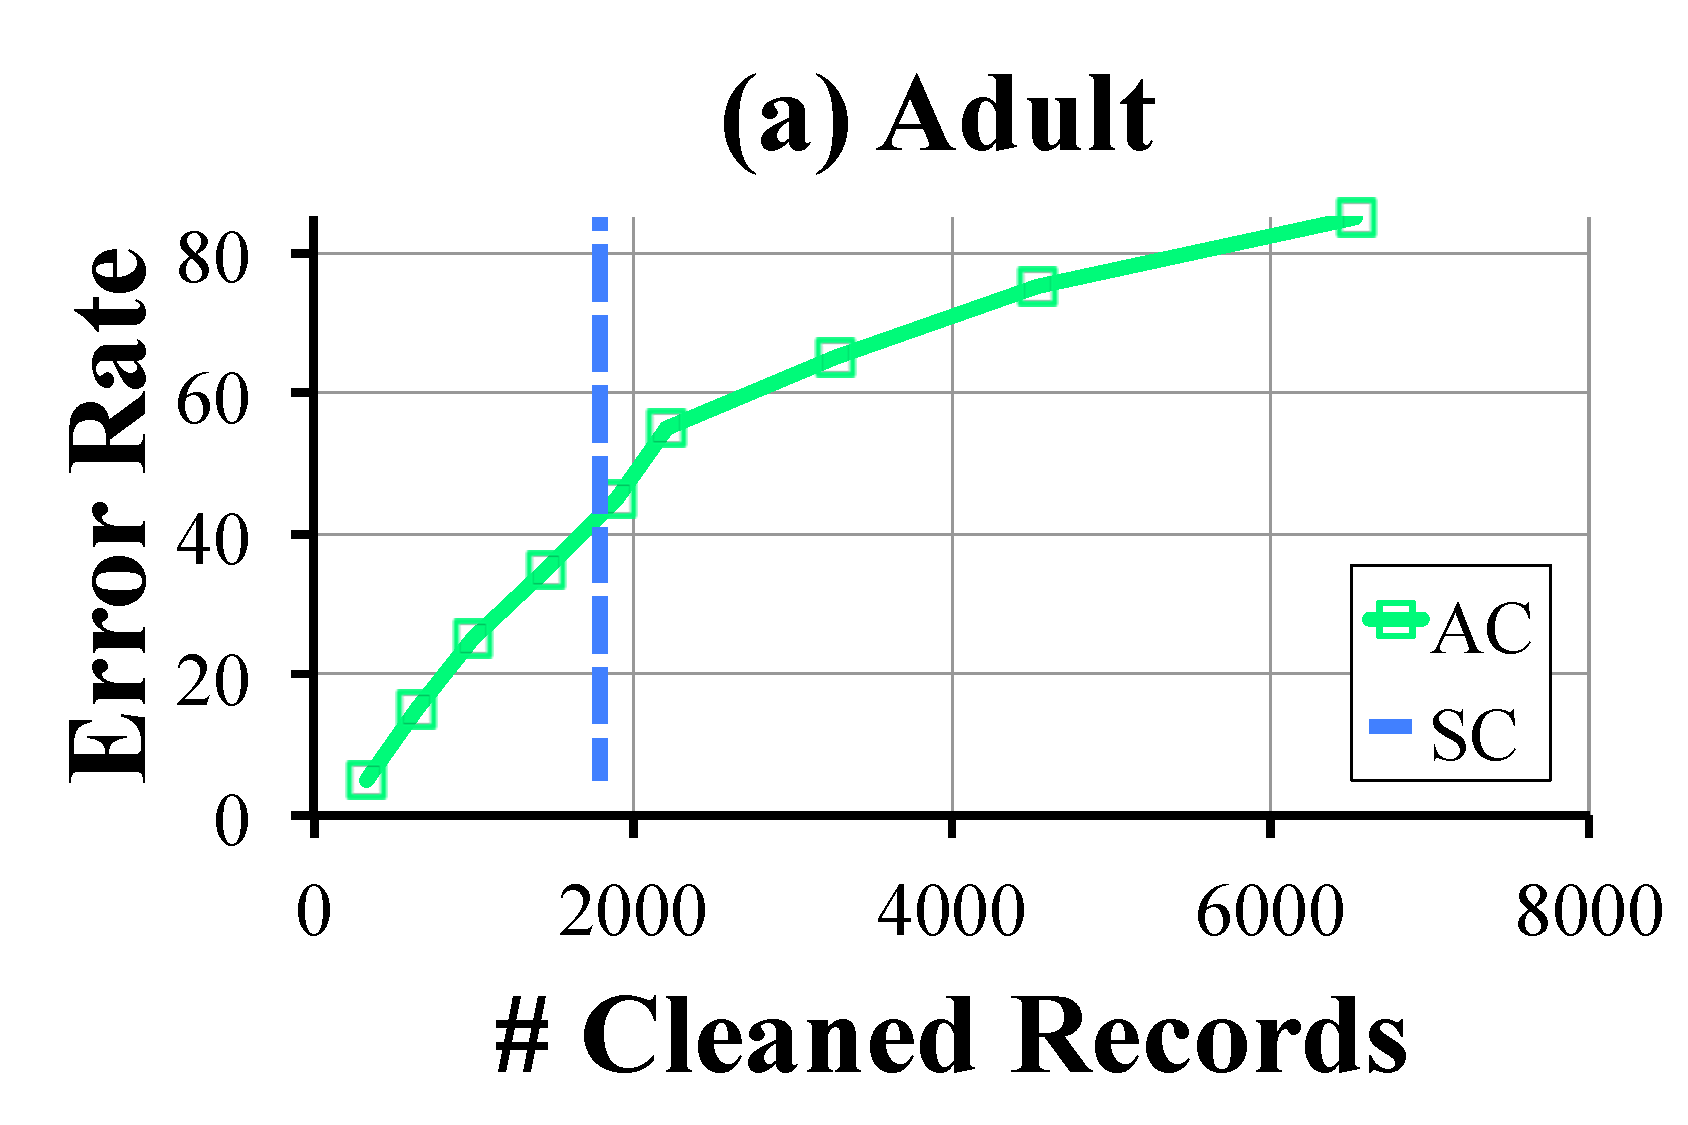
\includegraphics[width=0.49\columnwidth]{exp/exp9a.pdf}
  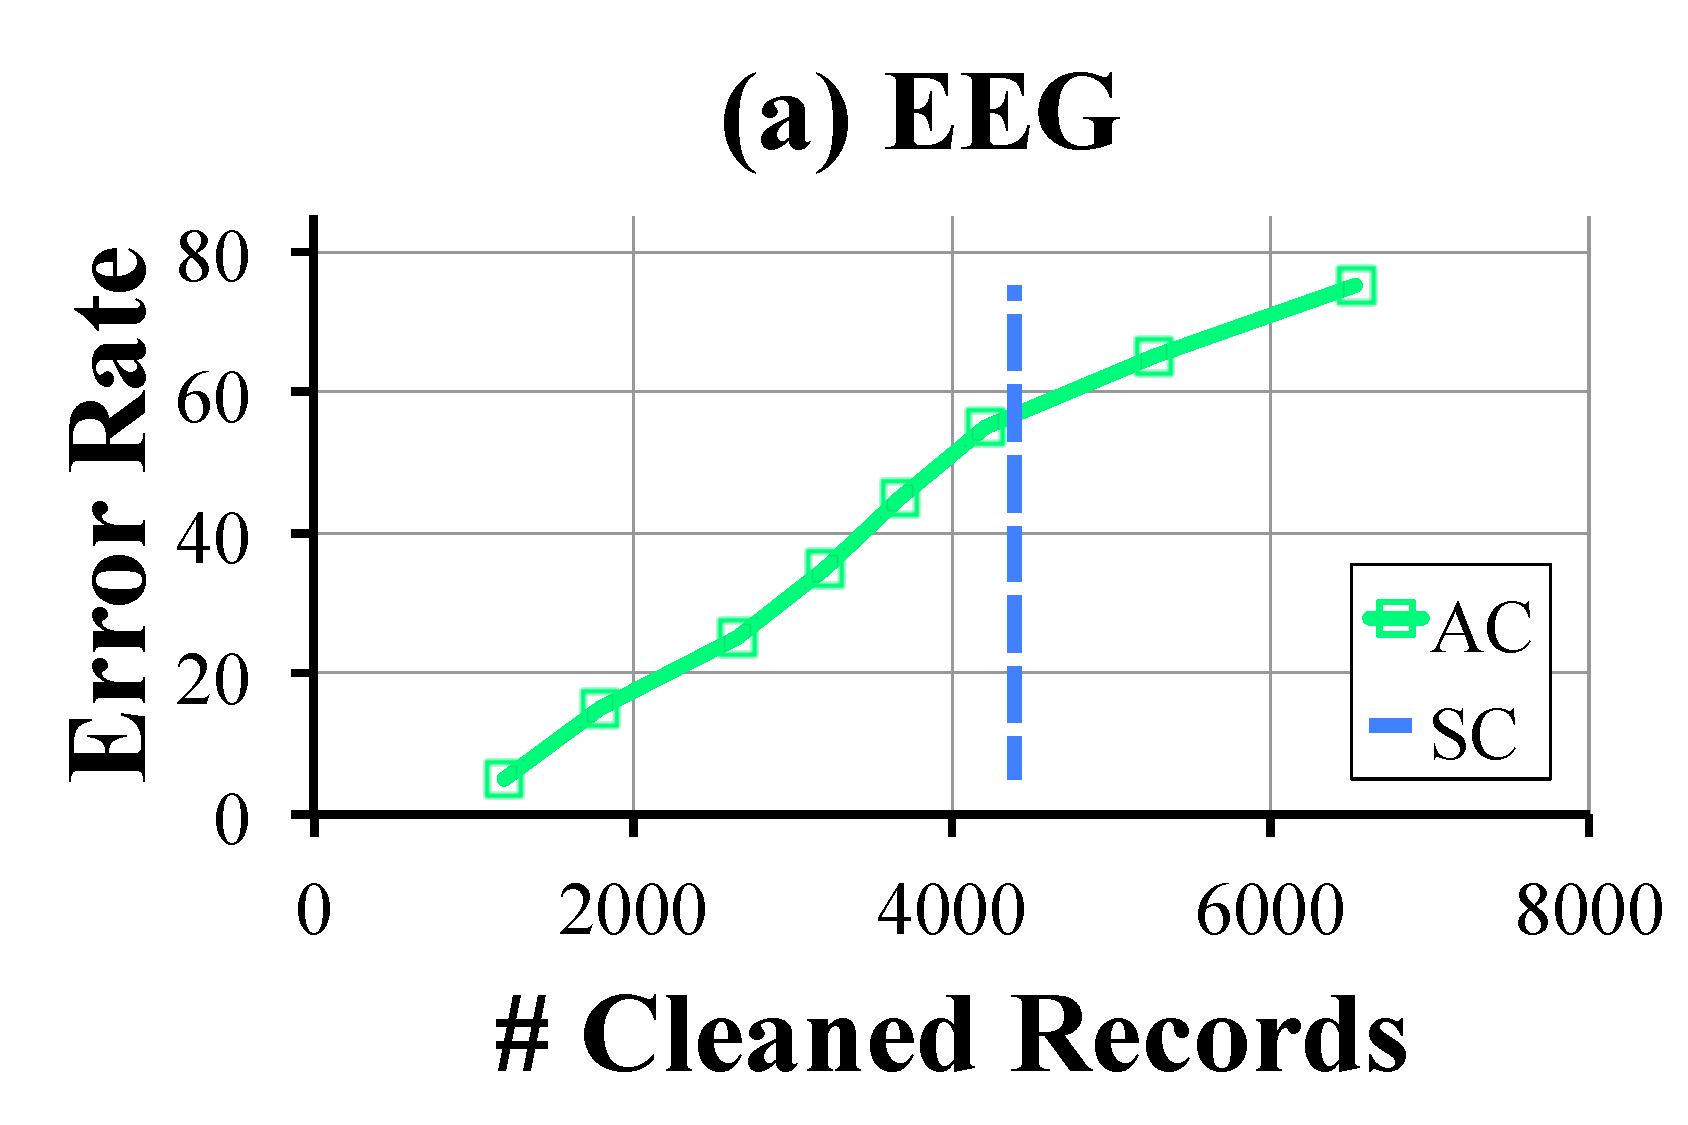
\includegraphics[width=0.49\columnwidth]{exp/exp9b.pdf}
 \caption{\sys performs well until the corruption is so severe that the dirty model is not a good initialization. The error of SampleClean does not depend on the corruption rate so it is a vertical line.  \label{bias}}
\end{figure}

\subsection{\sys: Adaptive Detection}
This experiment explores how the results of the previous experiment change when using an adaptive detector instead of the \emph{a priori} detector.
Recall, in the systematic corruption, 3 of the most informative features were corrupted, thus we group these problems into $9$ classes.
We use an all-versus-one SVM to learn the categorization.

\subsubsection{Basic Performance}
Figure \ref{pred-perf} overlays the convergence plots in the previous experiments with a curve (denoted by AC+C) that represents \sys using a classifier instead of the \emph{a priori} detection. Initially \sys is comparable to Active Learning; however, as the classifier becomes more effective the detection improves the performance.
Over both datasets, at the 500 records point on the curve, adaptive \sys has a 30\% higher model error compared to \emph{a priori} \sys.
At 1000 records point on the curve, adaptive \sys has about 10\% higher error.

\vspace{0.25em}

\noindent \emph{Summary: For 500 records cleaned, adaptive \sys has a 30\% higher model error compared to a priori \sys, but still outperforms Active Learning and SampleClean.}

\begin{figure}[t]
\centering\vspace{-1em}
 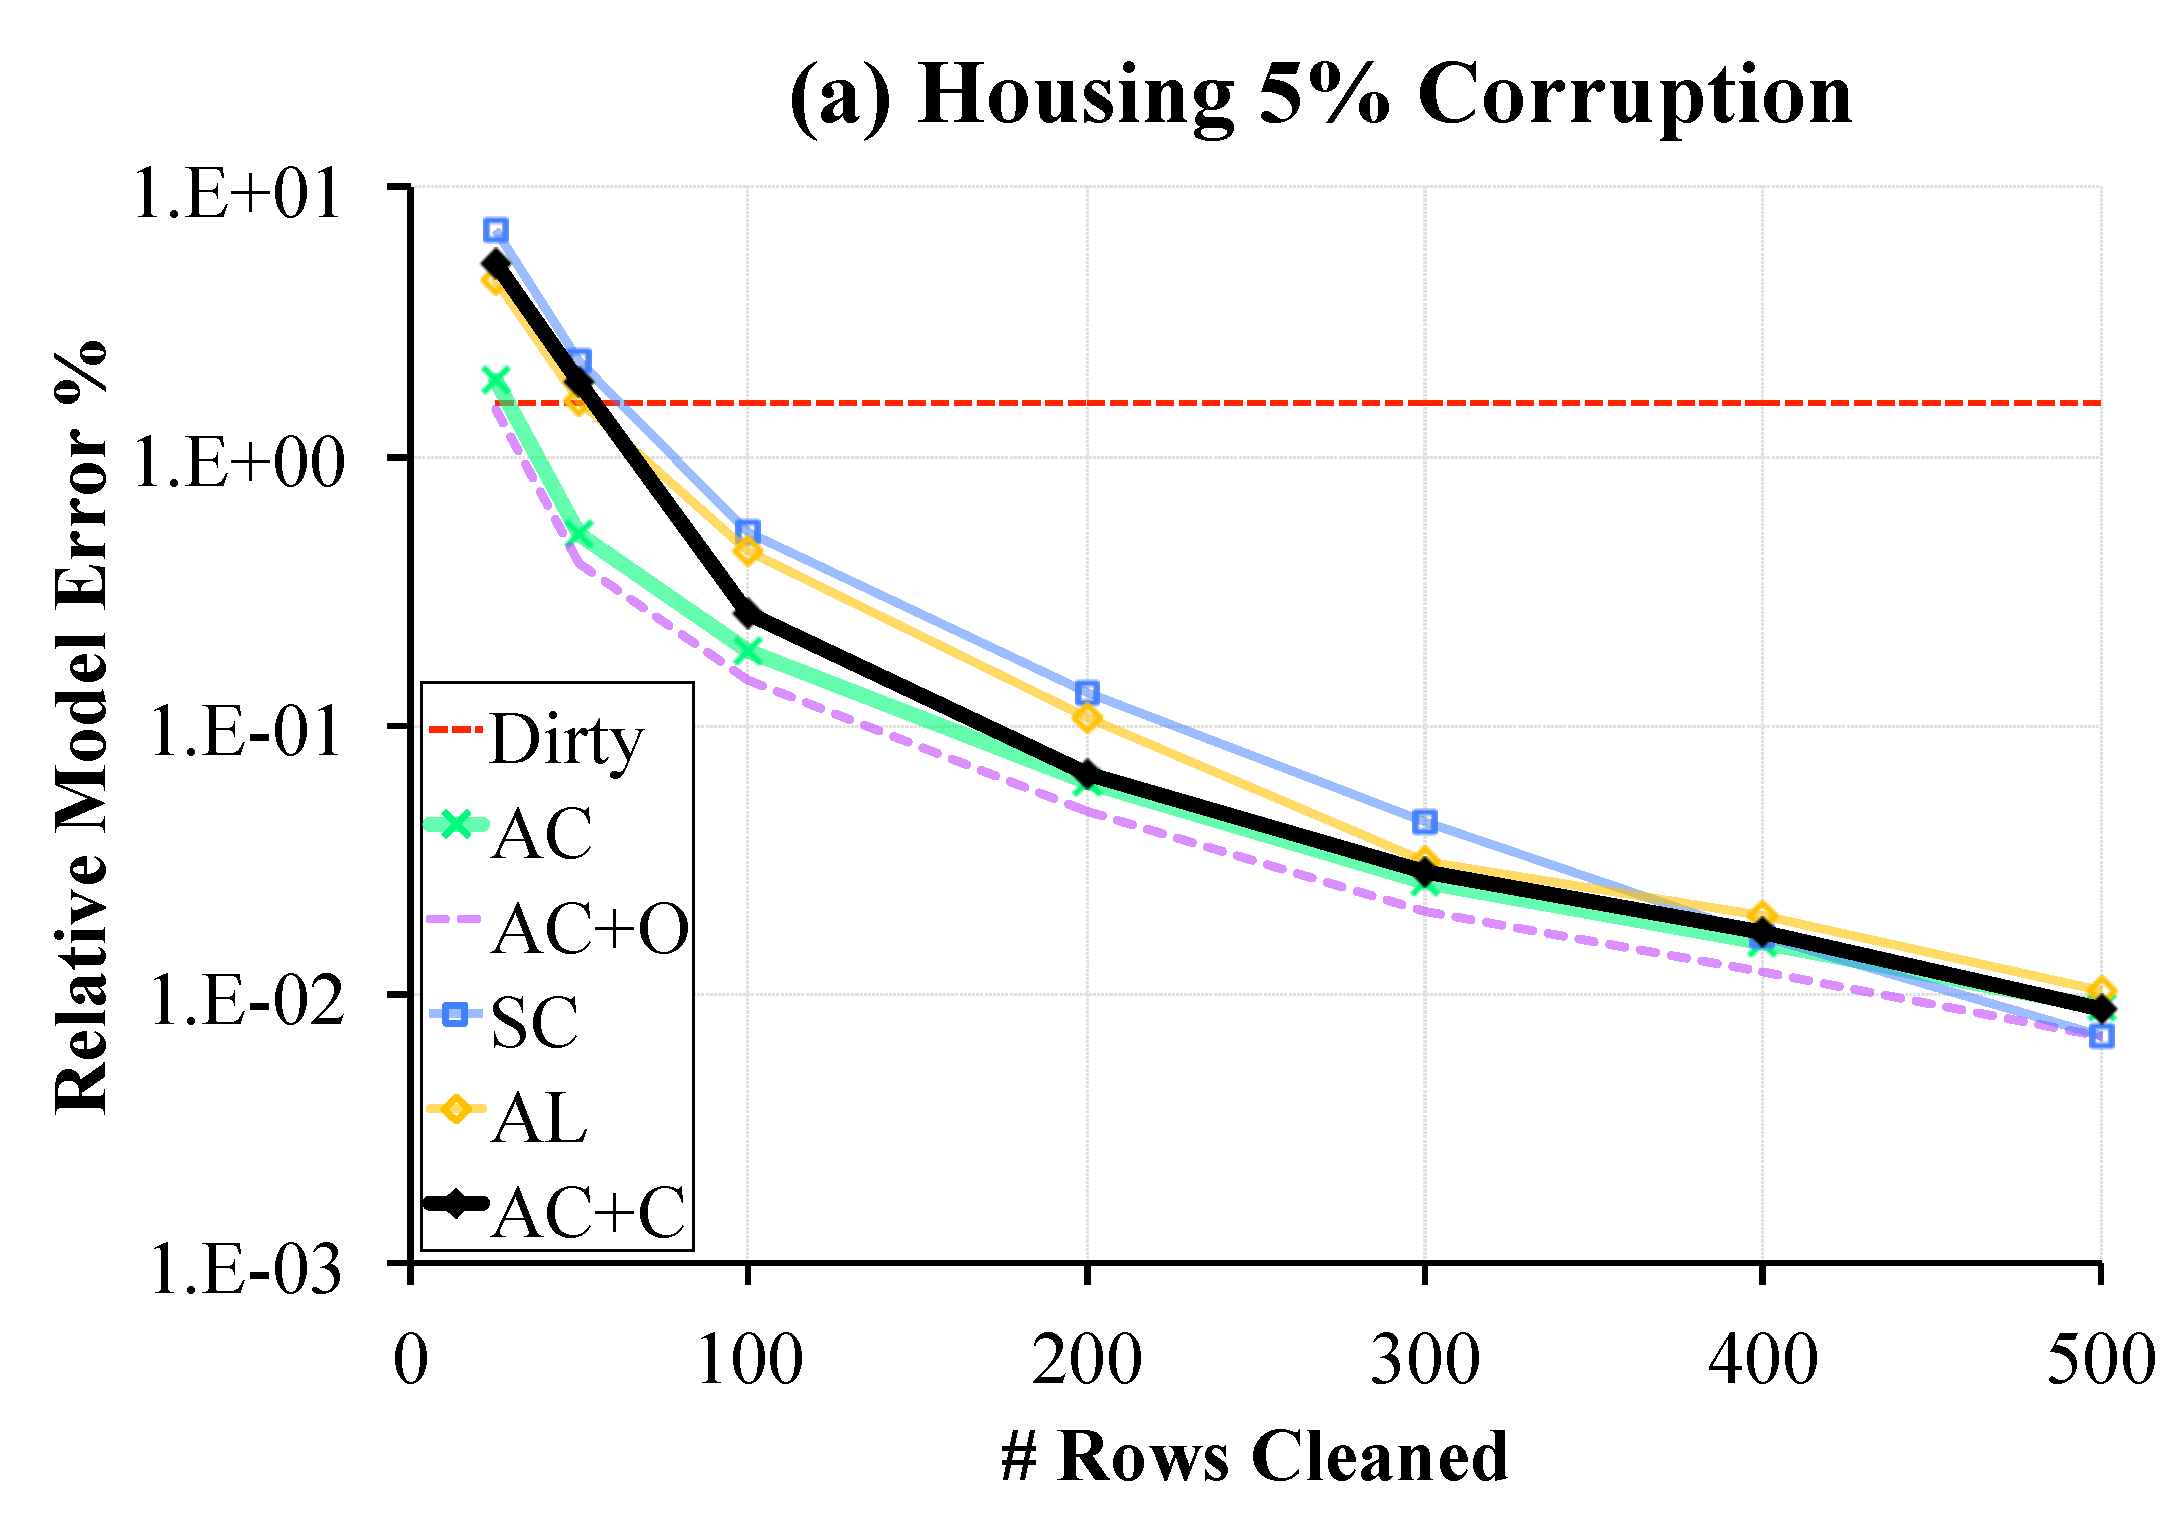
\includegraphics[width=0.49\columnwidth]{exp/exp11a.pdf}
 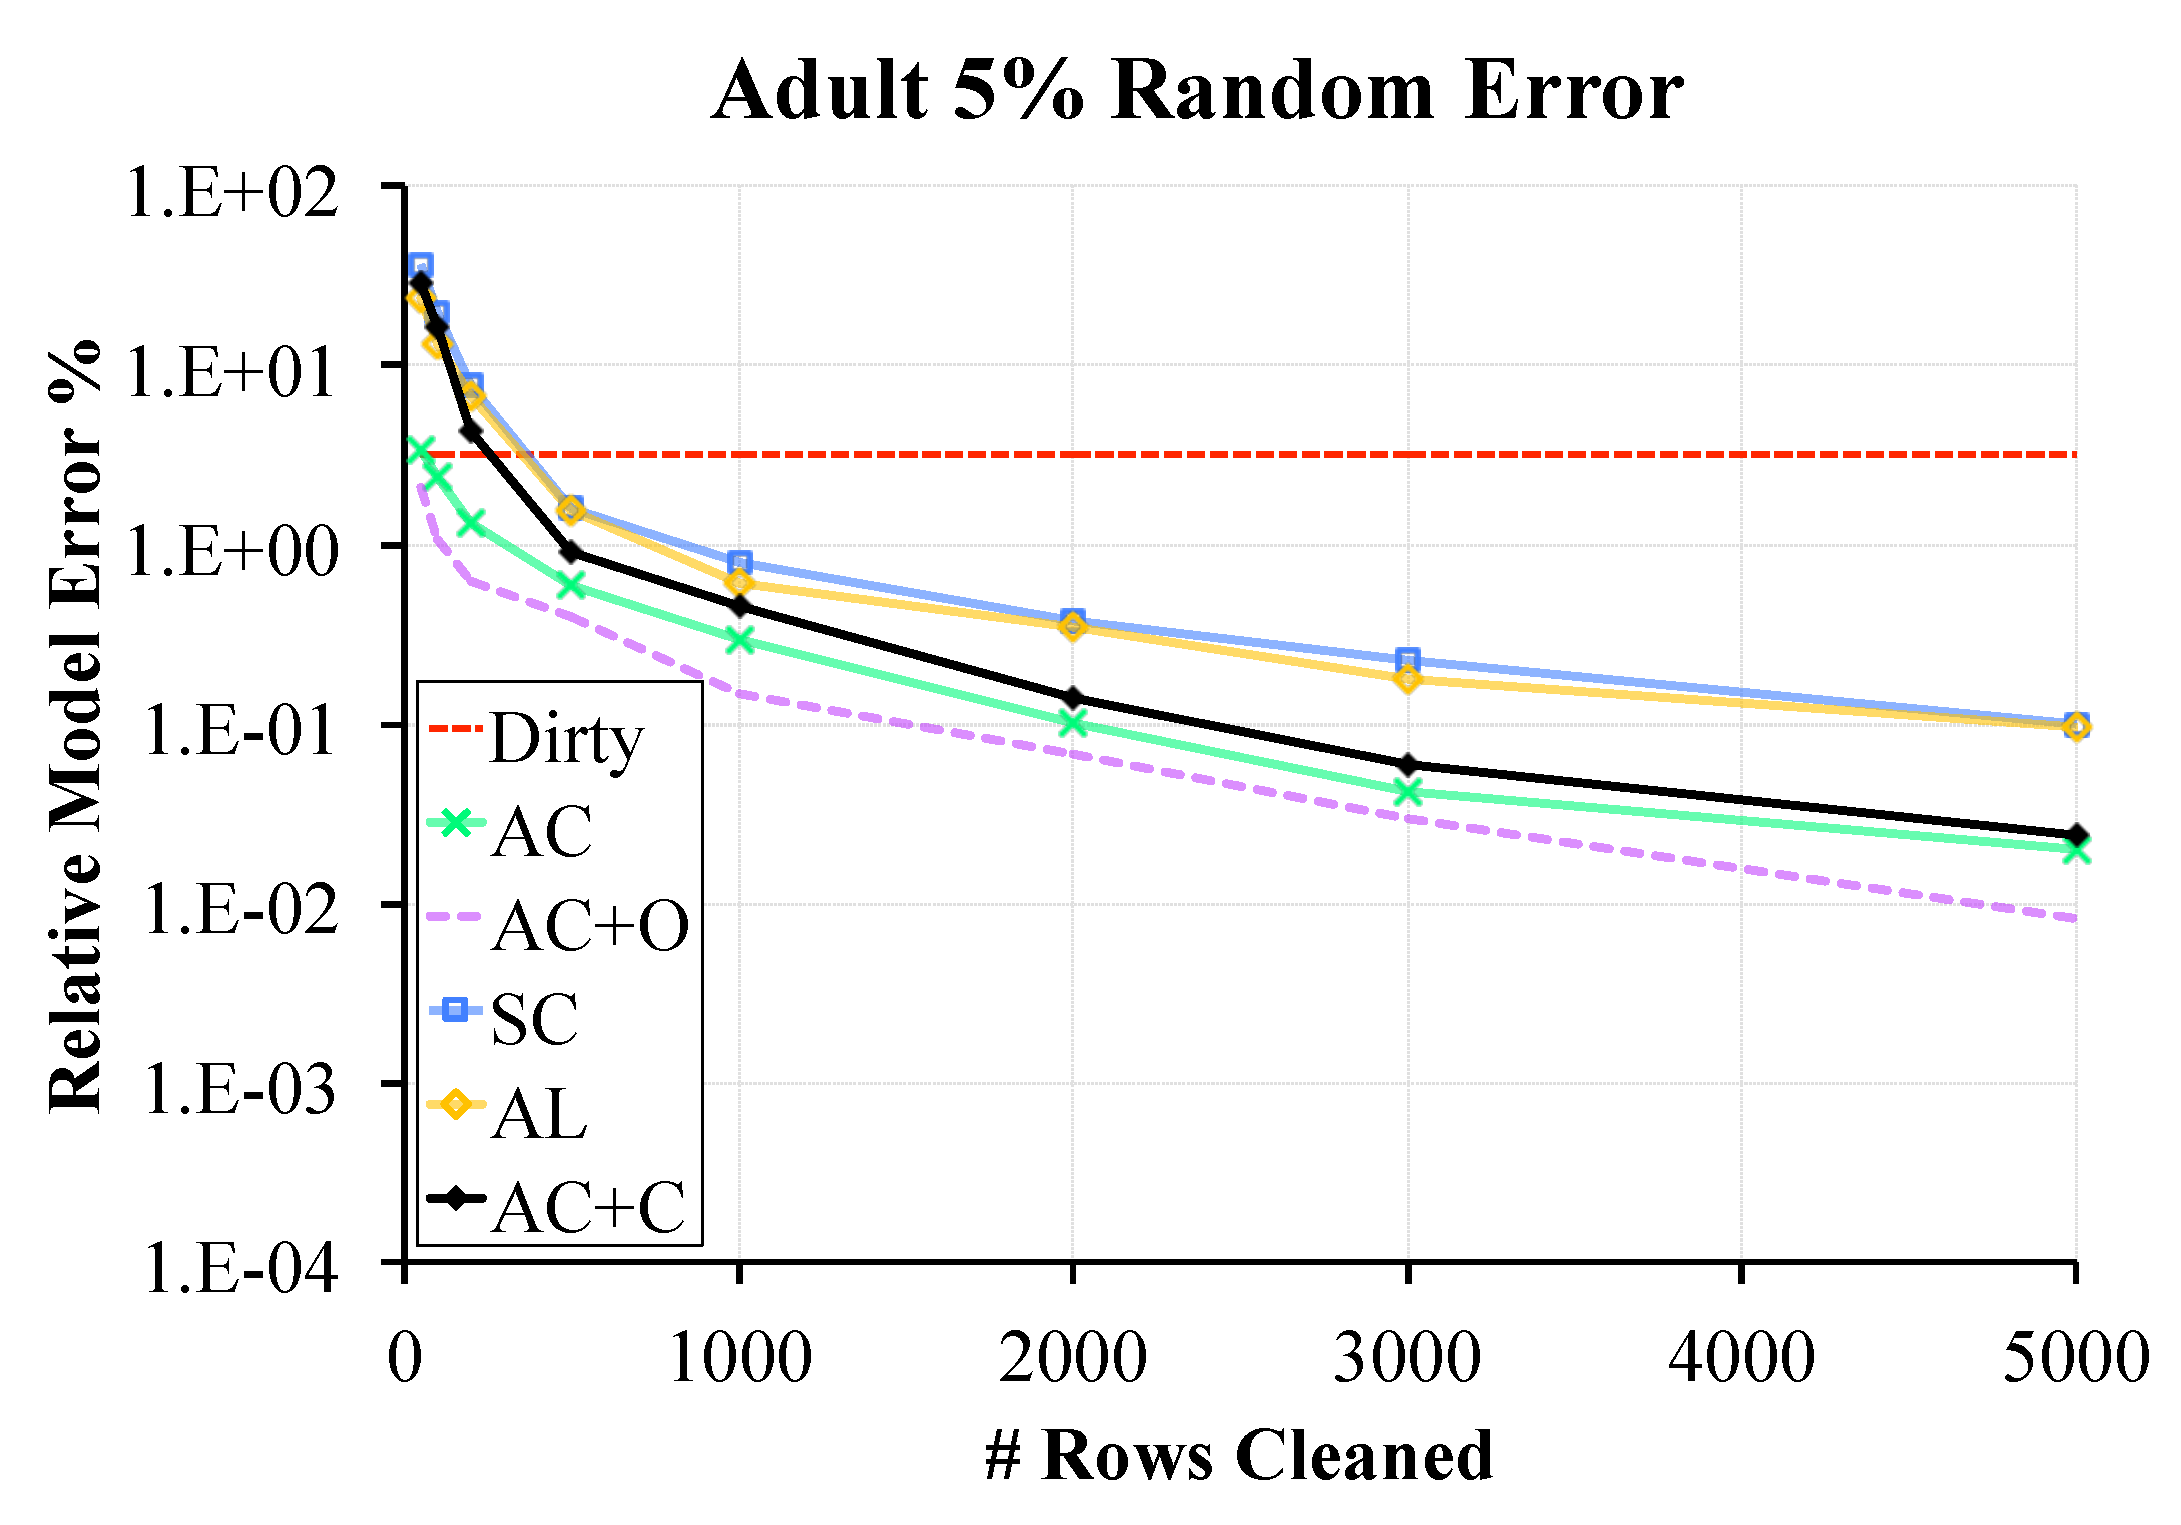
\includegraphics[width=0.49\columnwidth]{exp/exp11b.pdf}
 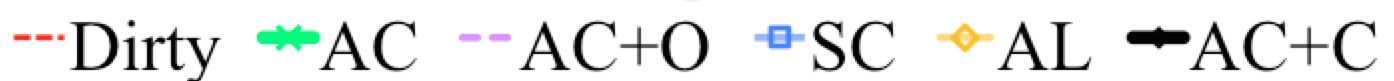
\includegraphics[width=0.49\columnwidth]{exp/legend-11.png}\vspace{-0.5em}
 \caption{Even with a classifier \sys converges faster than Active Learning and SampleClean. \label{pred-perf}}\vspace{-1.0em}
\end{figure}


\subsubsection{Classifiable Errors}
The adaptive case depends on being able to predict corrupted records.
For example, random corruption not correlated with any other data features may be hard to learn.
As corruption becomes more random, the classifier becomes increasingly erroneous.
The next experiment explores making the systematic corruption more random.
Instead of selecting the highest valued records for the most valuable features, we corrupt random records with probability $p$. 
We compare these results to AC-D where we do not have a detector at all at one vertical slice of the previous plot (cleaning 1000 records).
Figure \ref{tradeoffs2}a plots the relative error reduction using a classifier.
When the corruption is about 50\% random then there is a break even point where no detection is better.
This is because the classifier is imperfect and misclassifies some data points incorrectly as cleaned.

\vspace{0.25em}

\noindent \emph{Summary: When errors are increasingly random (50\% random) and cannot be accurately classified, adaptive detection provides no benefit over no detection. }

\begin{figure}[ht!]
\vspace{-1em}
\centering
 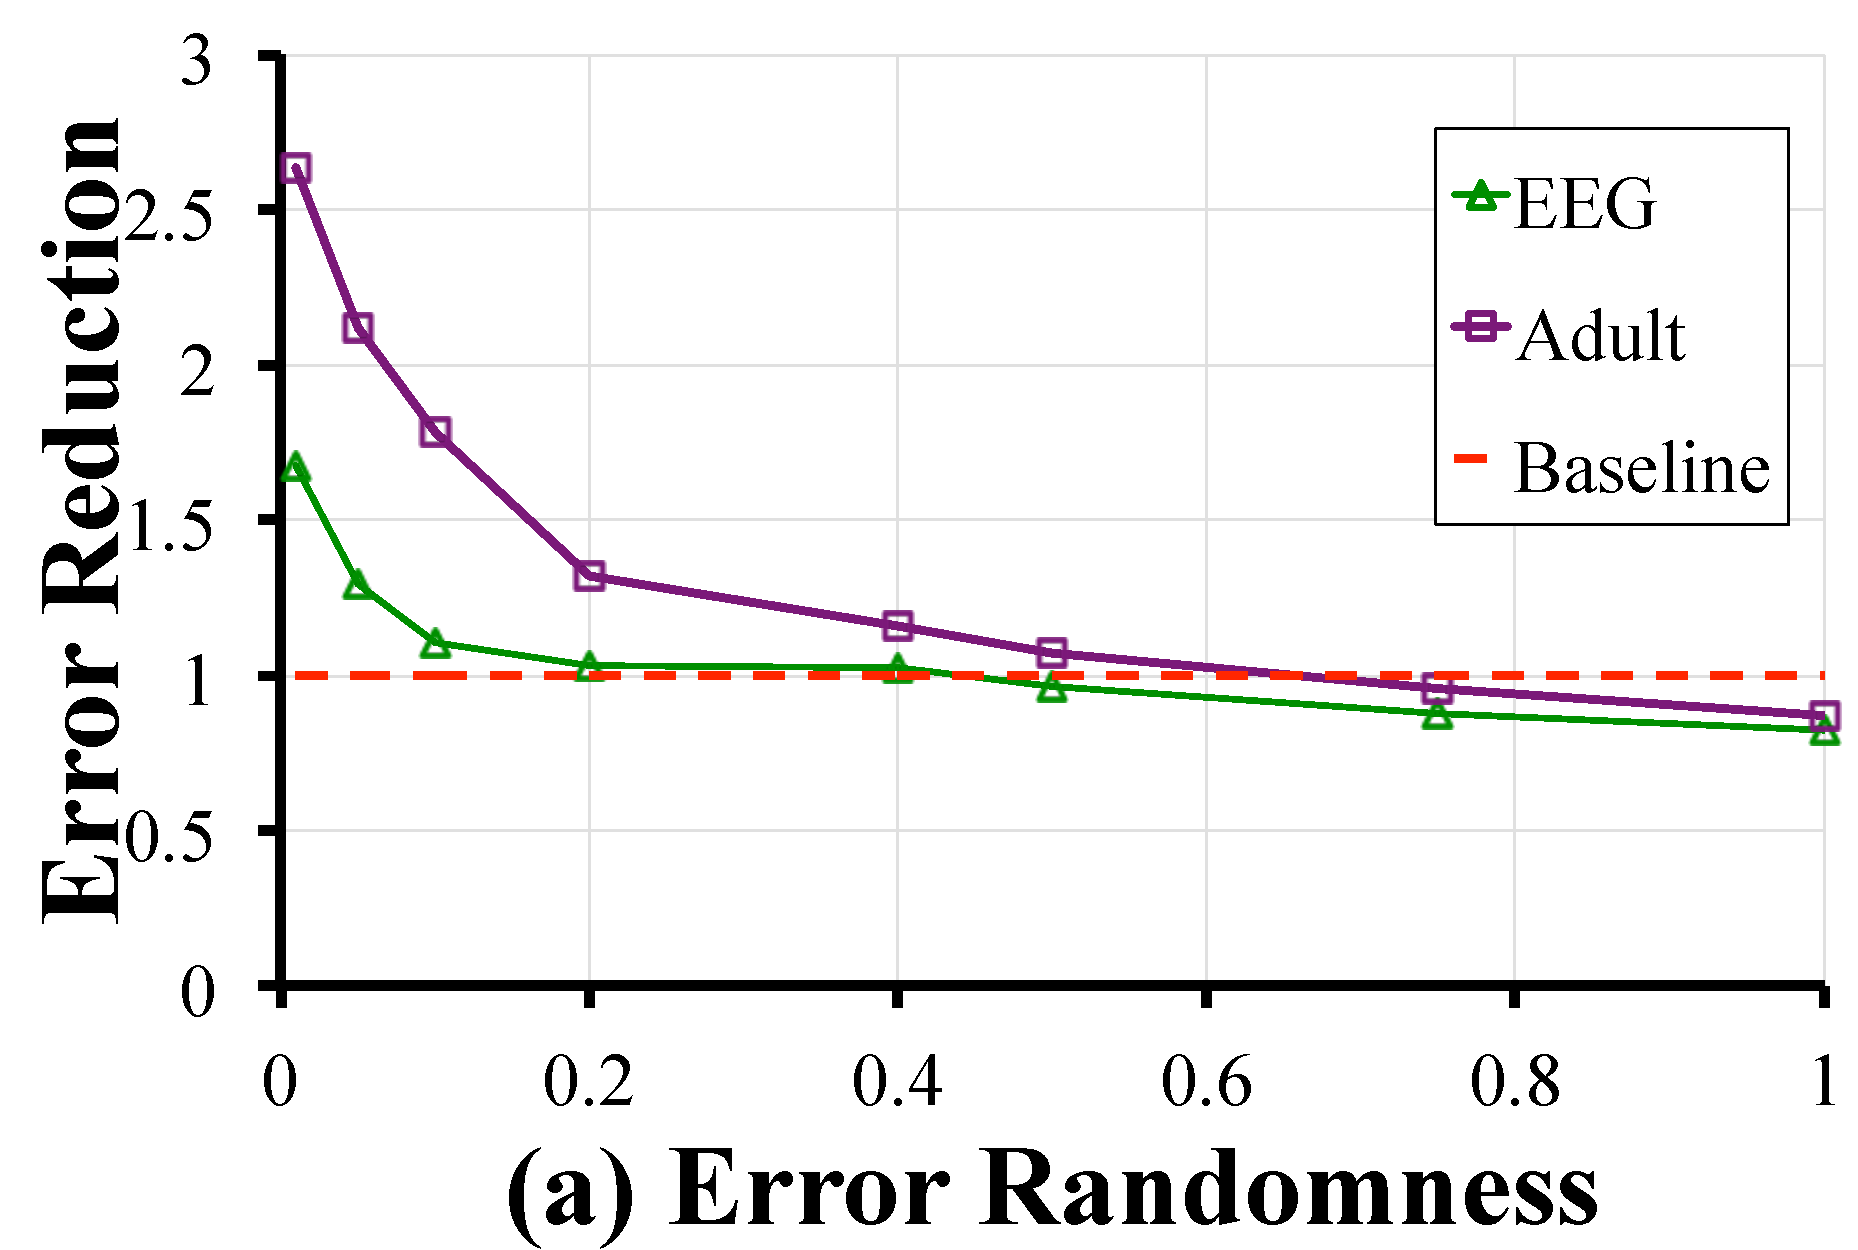
\includegraphics[width=0.49\columnwidth]{exp/exp5a.pdf}
 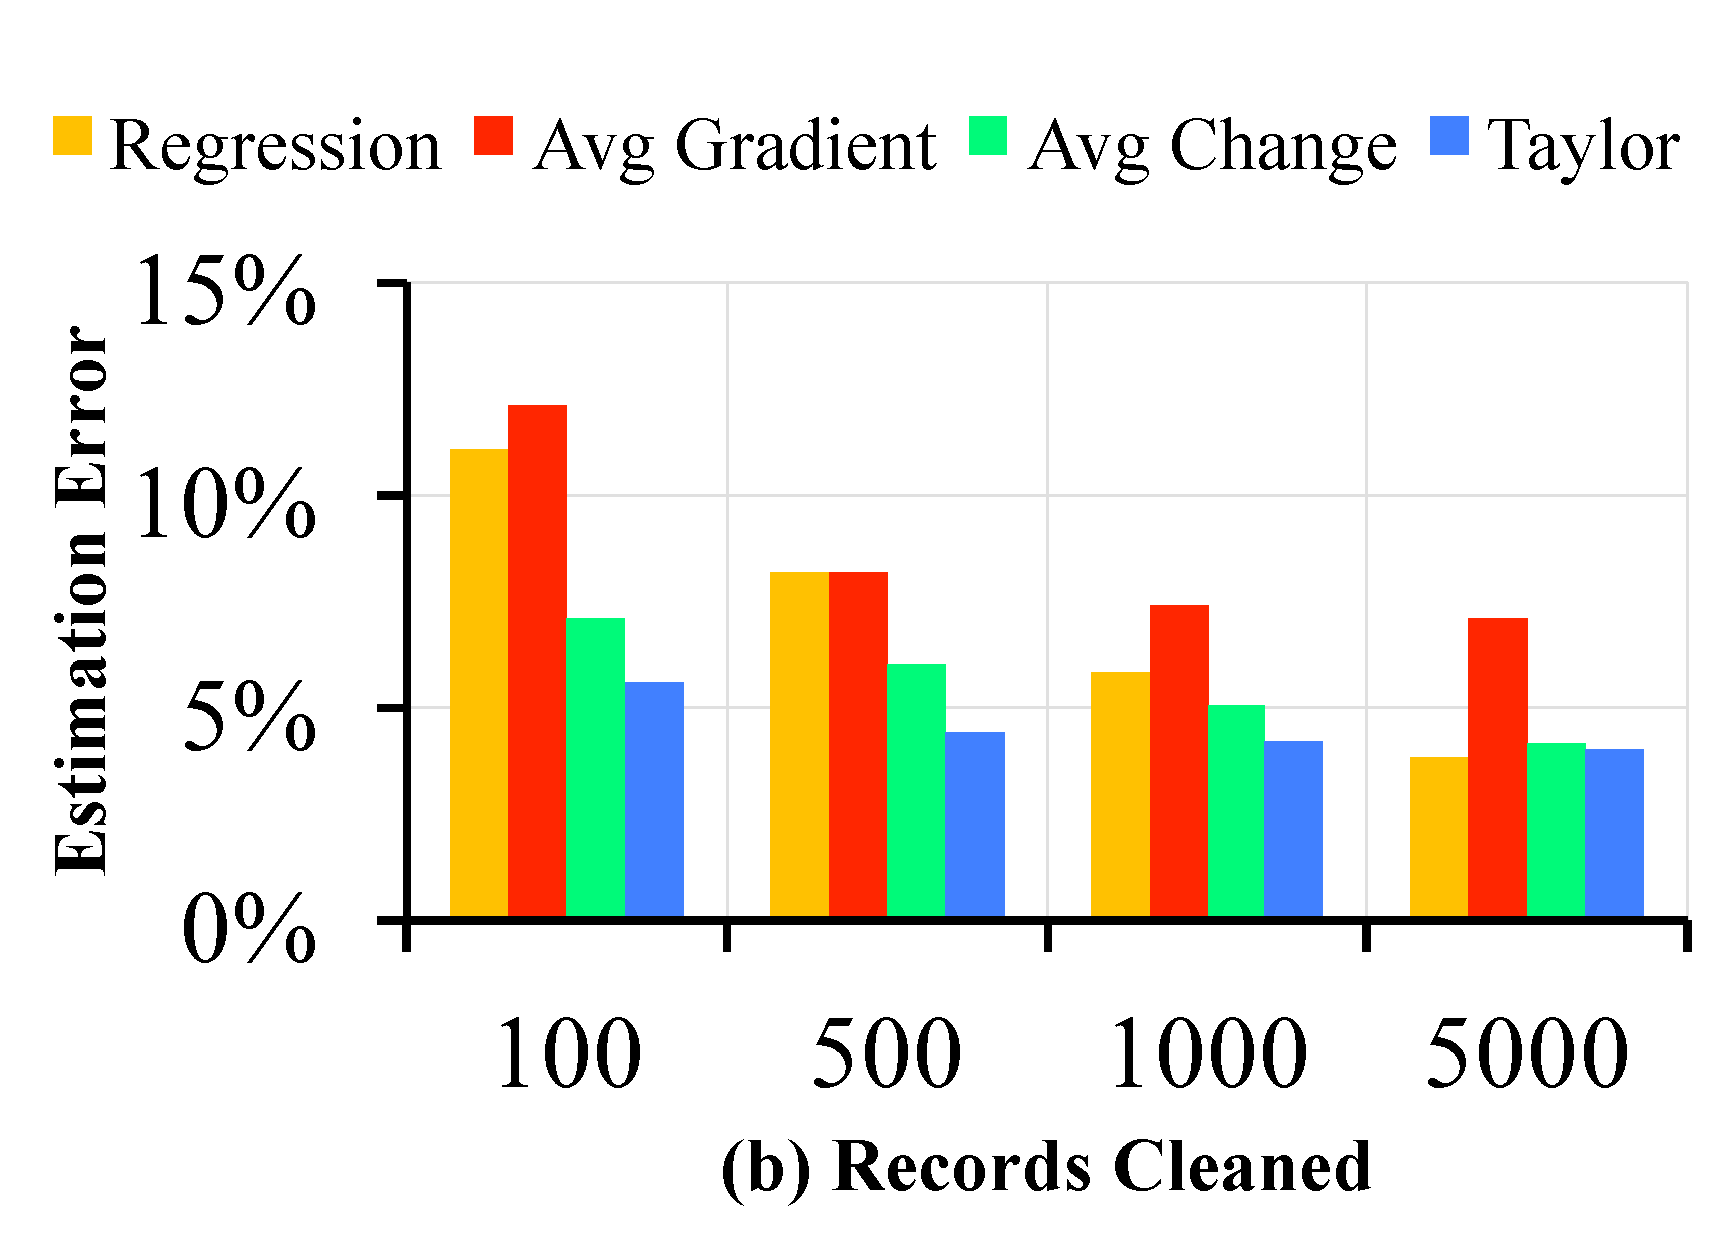
\includegraphics[width=0.49\columnwidth]{exp/exp12.pdf}
 \caption{(a) Data corruptions that are less random are easier to classify, and lead to more significant reductions in relative model error. (b) The Taylor series approximation gives more accurate estimates when the amount of cleaned data is small. \label{tradeoffs2}}
\end{figure}

\subsection{Estimation}\label{est}
The next experiment compares estimation techniques: (1) ``linear regression" trains a linear regression model that predicts the clean gradient as a function of the dirty gradient, (2) ``average gradient" which does not use the detection to inform how to apply the estimate, (3) ``average feature change" uses detection but no linearization, and (4) the Taylor series linear approximation.
Figure \ref{tradeoffs2}b measures how accurately each estimation technique estimates the gradient as a function of the number of cleaned records on the EEG dataset.

Estimation error is measured using the relative L2 error with the true gradient.
The Taylor series approximation proposed gives more accurate for small cleaning sizes, confirming the analysis in Section \ref{acc}.
Linear regression and the average feature change technique do eventually perform comparably but only after cleaning much more data.

\vspace{0.25em}

\noindent \emph{Summary: Linearized gradient estimates are more accurate when estimated from small samples. }

\subsection{Real World Scenarios}
The next set of experiments evaluate \sys in two real world scenarios, one demonstrating the \emph{a priori} case and the other for the adaptive detection case.

\subsubsection{A Priori: Constraint Cleaning}\label{dfd-exp}
The first scenario explores the Dollars for Docs dataset published by ProPublica described throughout the paper.
To run this experiment, the entire dataset was cleaned up front, and simulated sampling from the dirty data and cleaning by looking up the value in the cleaned data (see Appendix \ref{dfd-errors} for constraints, errors, and cleaning methodology).
Figure \ref{dfd}a shows that \sys converges faster than Active Learning and SampleClean.
To achieve a 4\% relative error (i.e., a 75\% error reduction from the dirty model), \sys cleans 40000 fewer records than Active Learning.
Also, for 10000 records cleaned, \sys has nearly an order of magnitude smaller error than SampleClean.

Figure \ref{dfd}b shows the detection rate (fraction of disallowed research contributions identified) of the classifier as a function of the number of records cleaned. 
On the dirty data, we can only correctly classify 66\% of the suspected examples (88\% overall accuracy due to a class imbalance).
On the cleaned data, this classifier is nearly perfect with a 97\% true positive rate (98\% overall accuracy).
\sys converges to the cleaned accuracy faster than the alternatives with a classifier of 92\% true positive rate for only 10000 records cleaned.

\vspace{0.25em}

\noindent \emph{Summary: To achieve an 80\% detection rate, \sys cleans nearly 10x less records than Active Learning. }

\begin{figure}[ht!]
\centering
 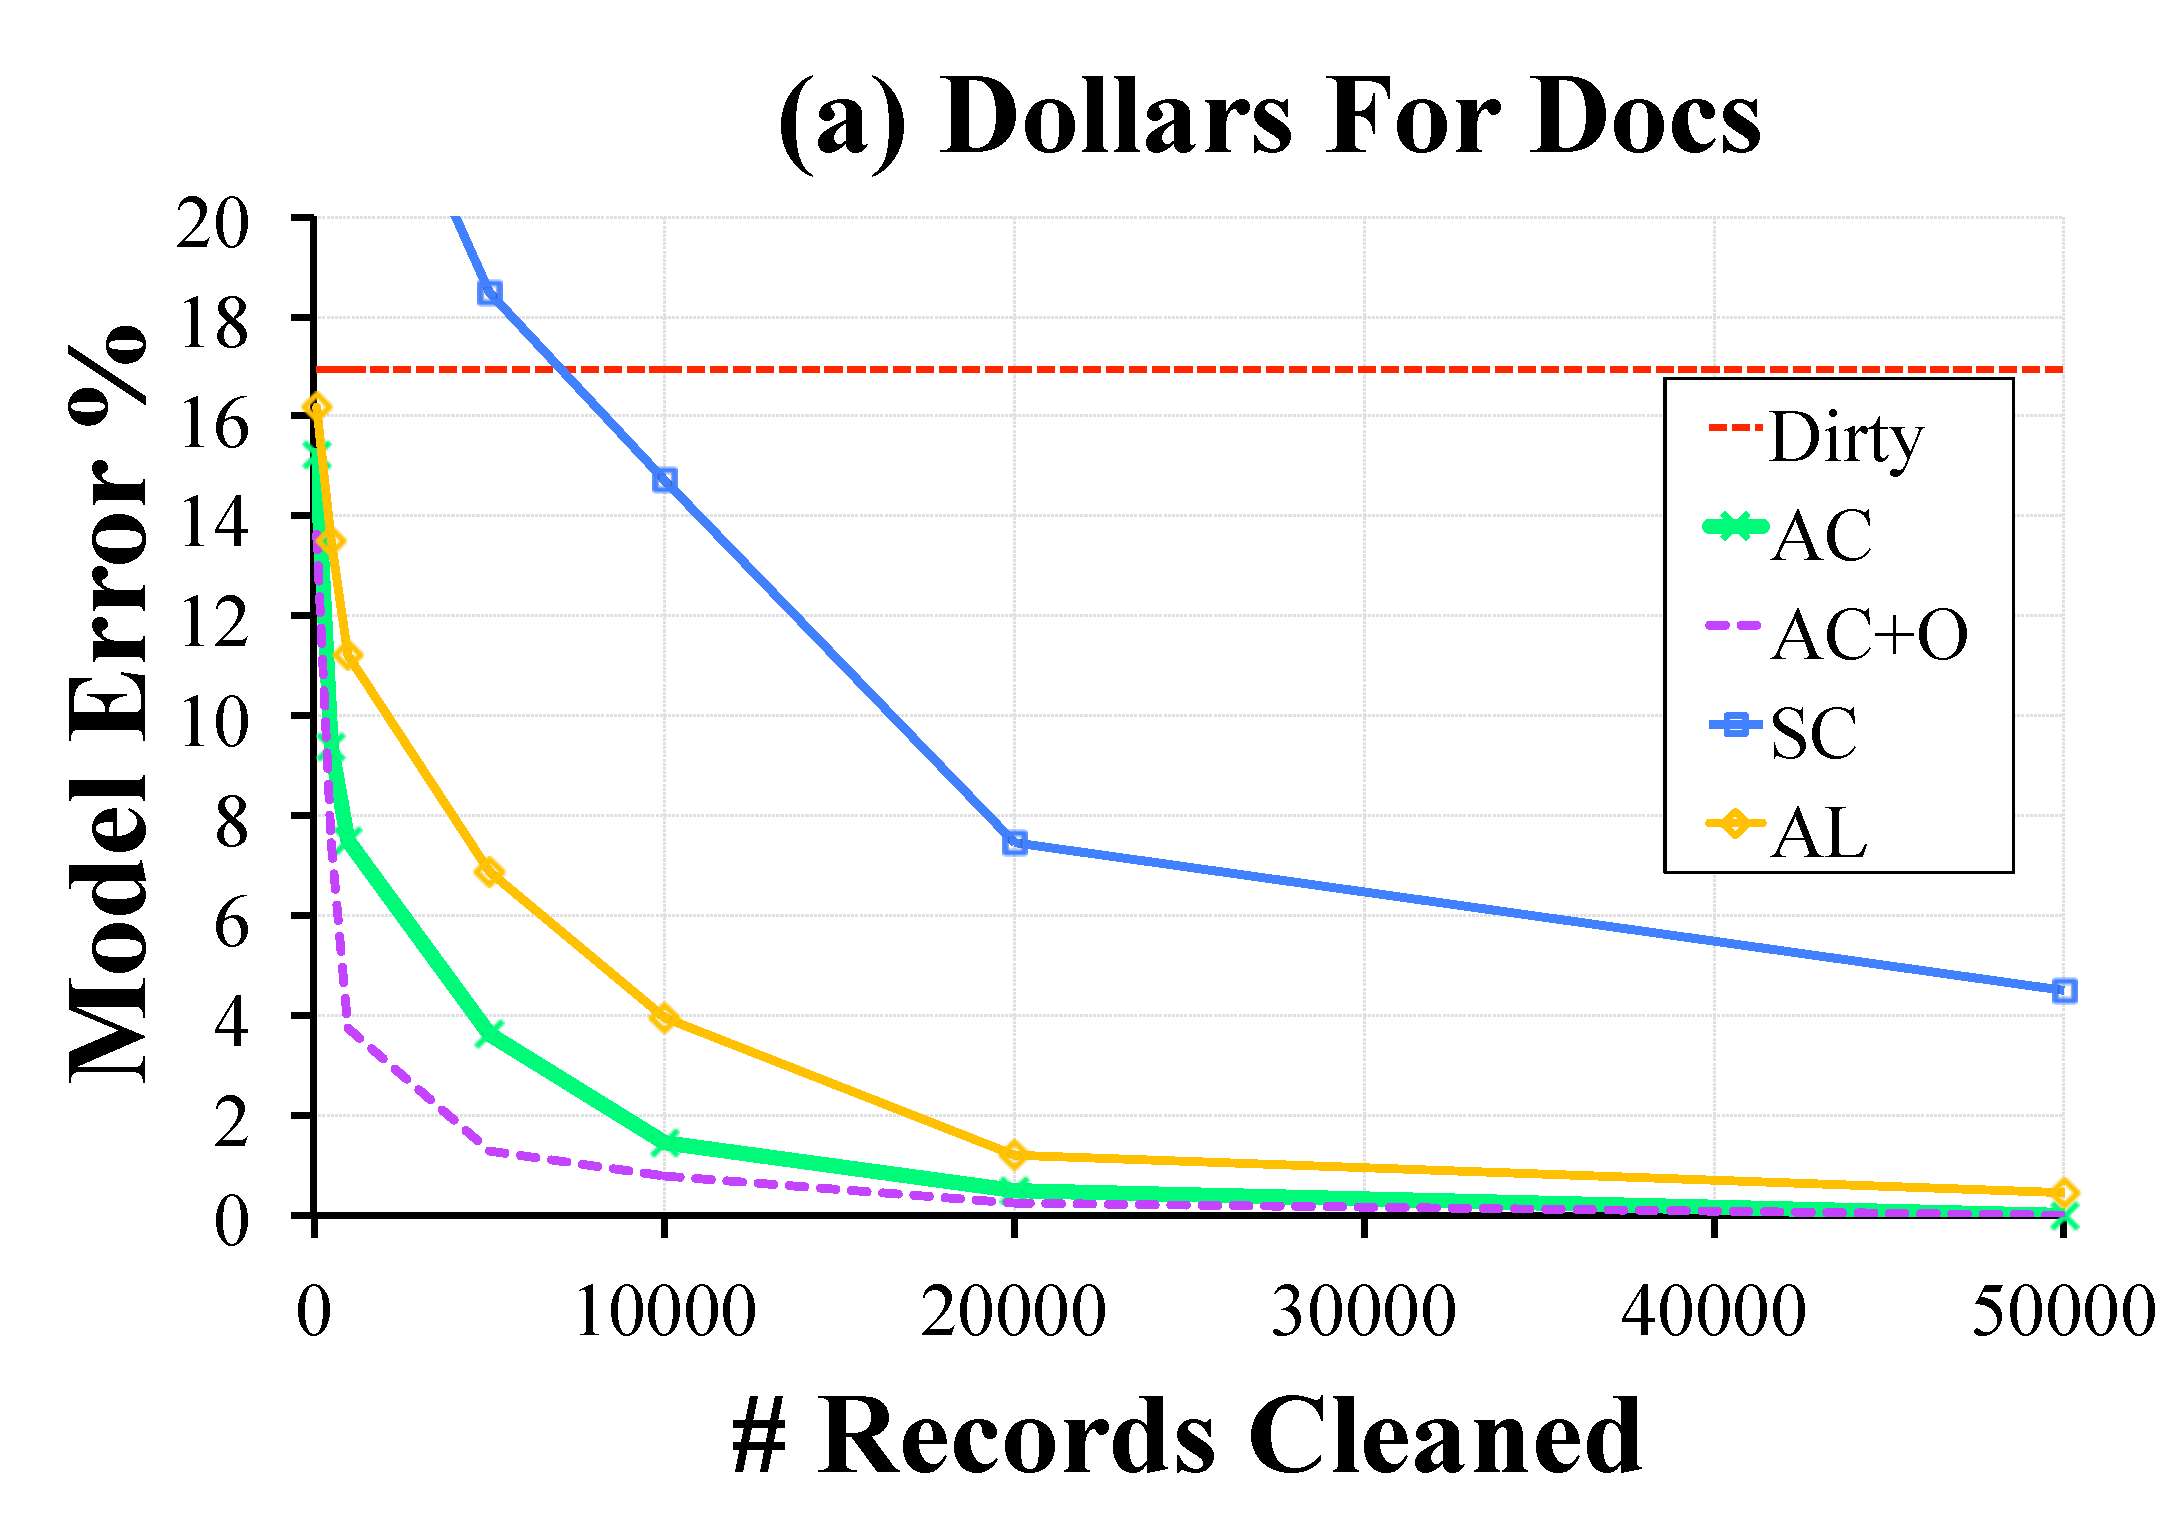
\includegraphics[width=0.49\columnwidth]{exp/exp13a.pdf}
 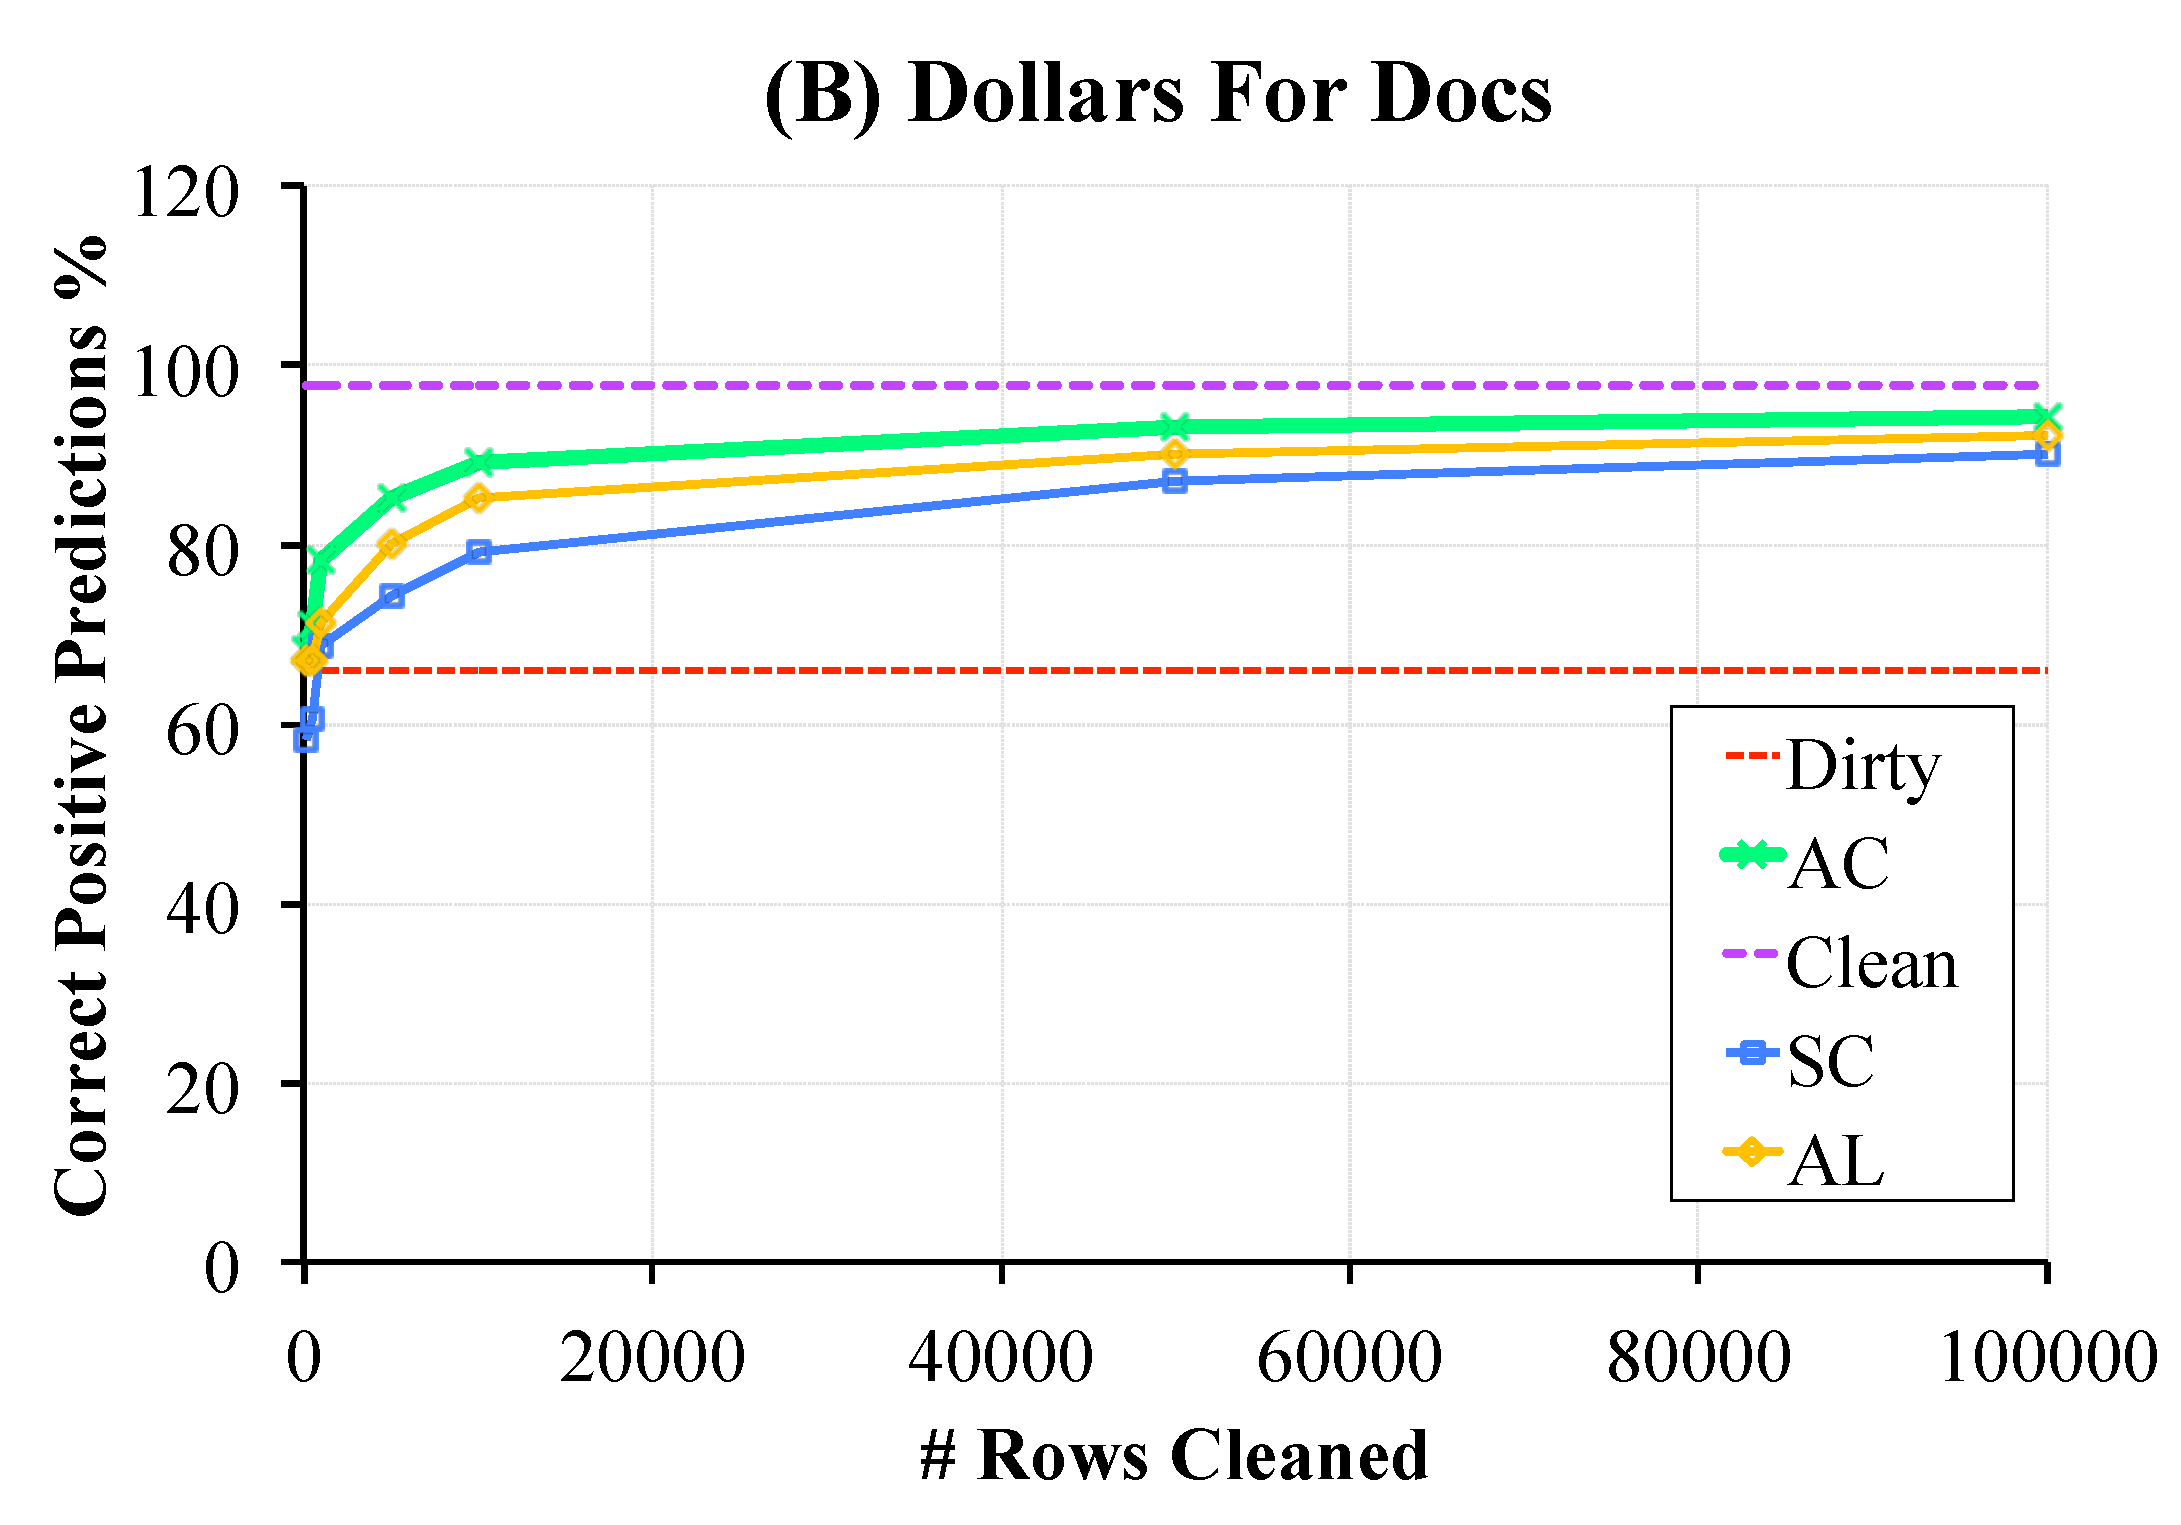
\includegraphics[width=0.49\columnwidth]{exp/exp13b.pdf}\vspace{-1em}
 \caption{(a) The relative model error as a function of the number of cleaned records. (b) The true positive rate as a function of the number of cleaned records. \label{dfd}}\vspace{-1em}
\end{figure}

\subsubsection{Adaptive: Replacing Corrupted Data}
The next experiment explores the MNIST handwritten digit recognition dataset with a MATLAB image processing pipeline.
In this scenario, the analyst must inspect a potentially corrupted image and replace it with a higher quality one.
The MNIST dataset consists of 64x64 grayscale images.
There are two types of simulated corruptions: (1) 5x5 block removal where a random 5x5 block is removed from the image by setting its pixel values to 0, and (2) Fuzzy where a 4x4 moving average patch is applied over the entire image.
These corruptions are applied to a random 5\% of the images, and mimic the random (Fuzzy) vs. systematic corruption (5x5 removal) studied in the previous experiments.
The adaptive detector uses a 10 class classifier (one for each digit) to detect the corruption.

Figure \ref{mnist} shows that \sys makes more progress towards the clean model with a smaller number of examples cleaned.
To achieve a 2\% error for the block removal, \sys can inspect 2200 fewer images than Active Learning and 2750 fewer images than SampleClean.
For the fuzzy images, both Active Learning and \sys reach 2\% error after cleaning fewer than 100 images, while SampleClean requires 1750.

\vspace{0.25em}

\noindent \emph{Summary: In the MNIST dataset, \sys significantly reduces (more than 2x) the number of images to clean to train a model with 2\% error. }

\begin{figure}[ht]
\centering\vspace{-0.5em}
 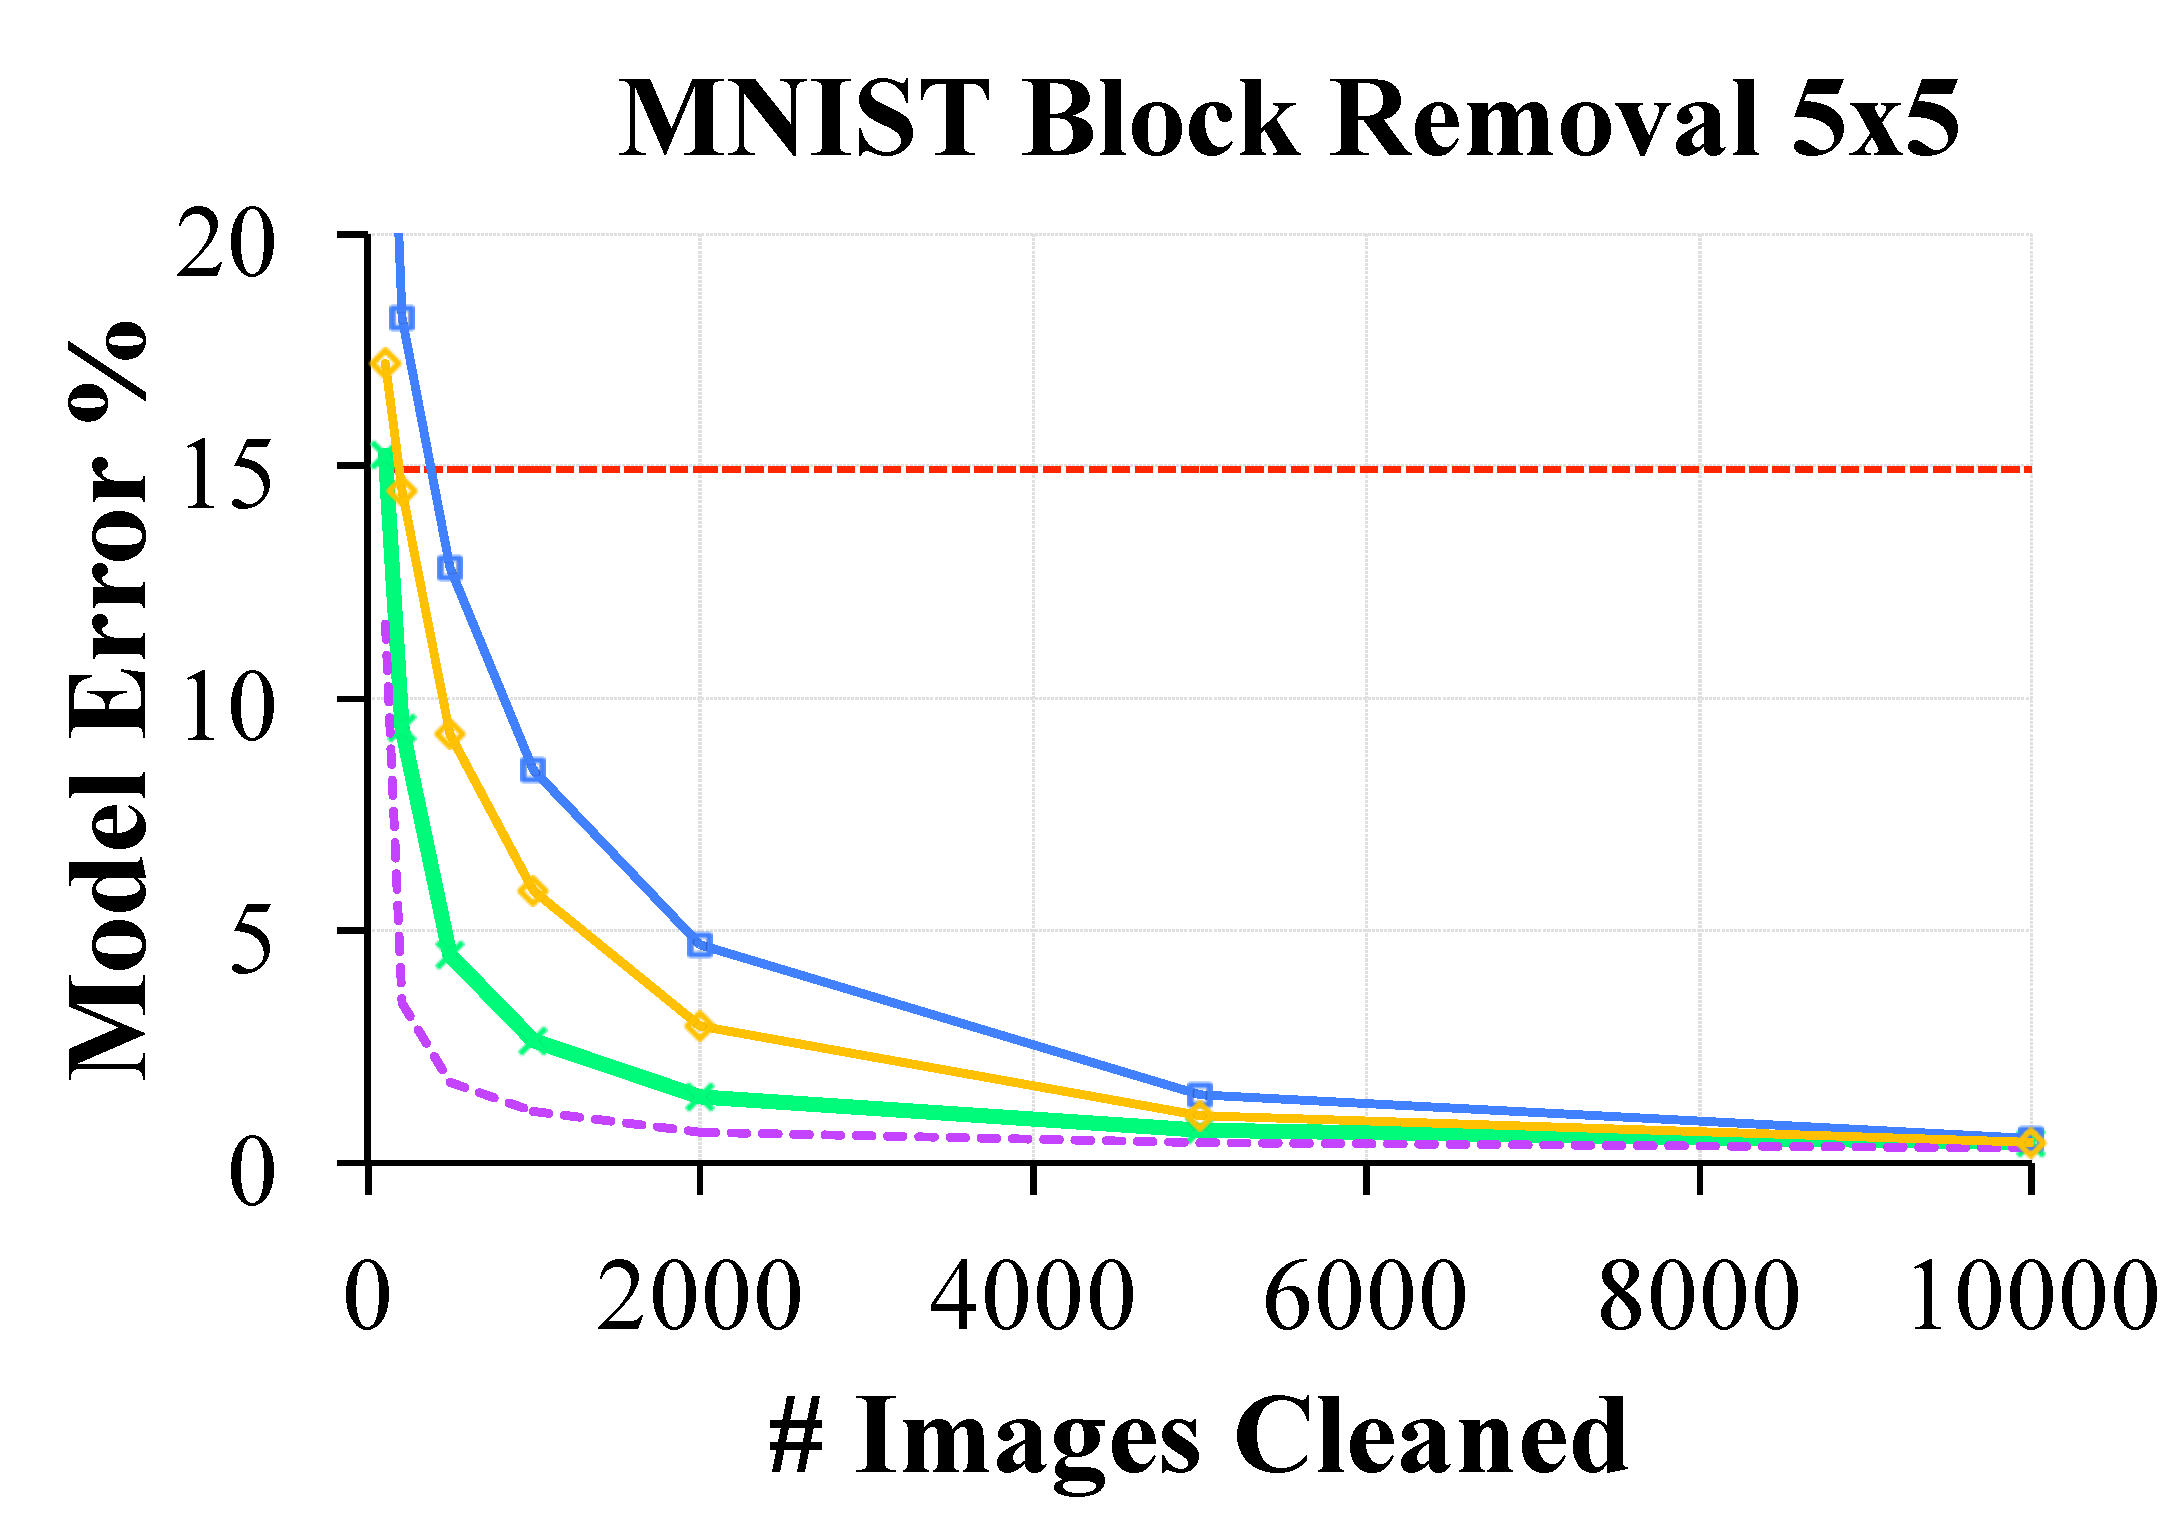
\includegraphics[width=0.49\columnwidth]{exp/exp7a.pdf}
 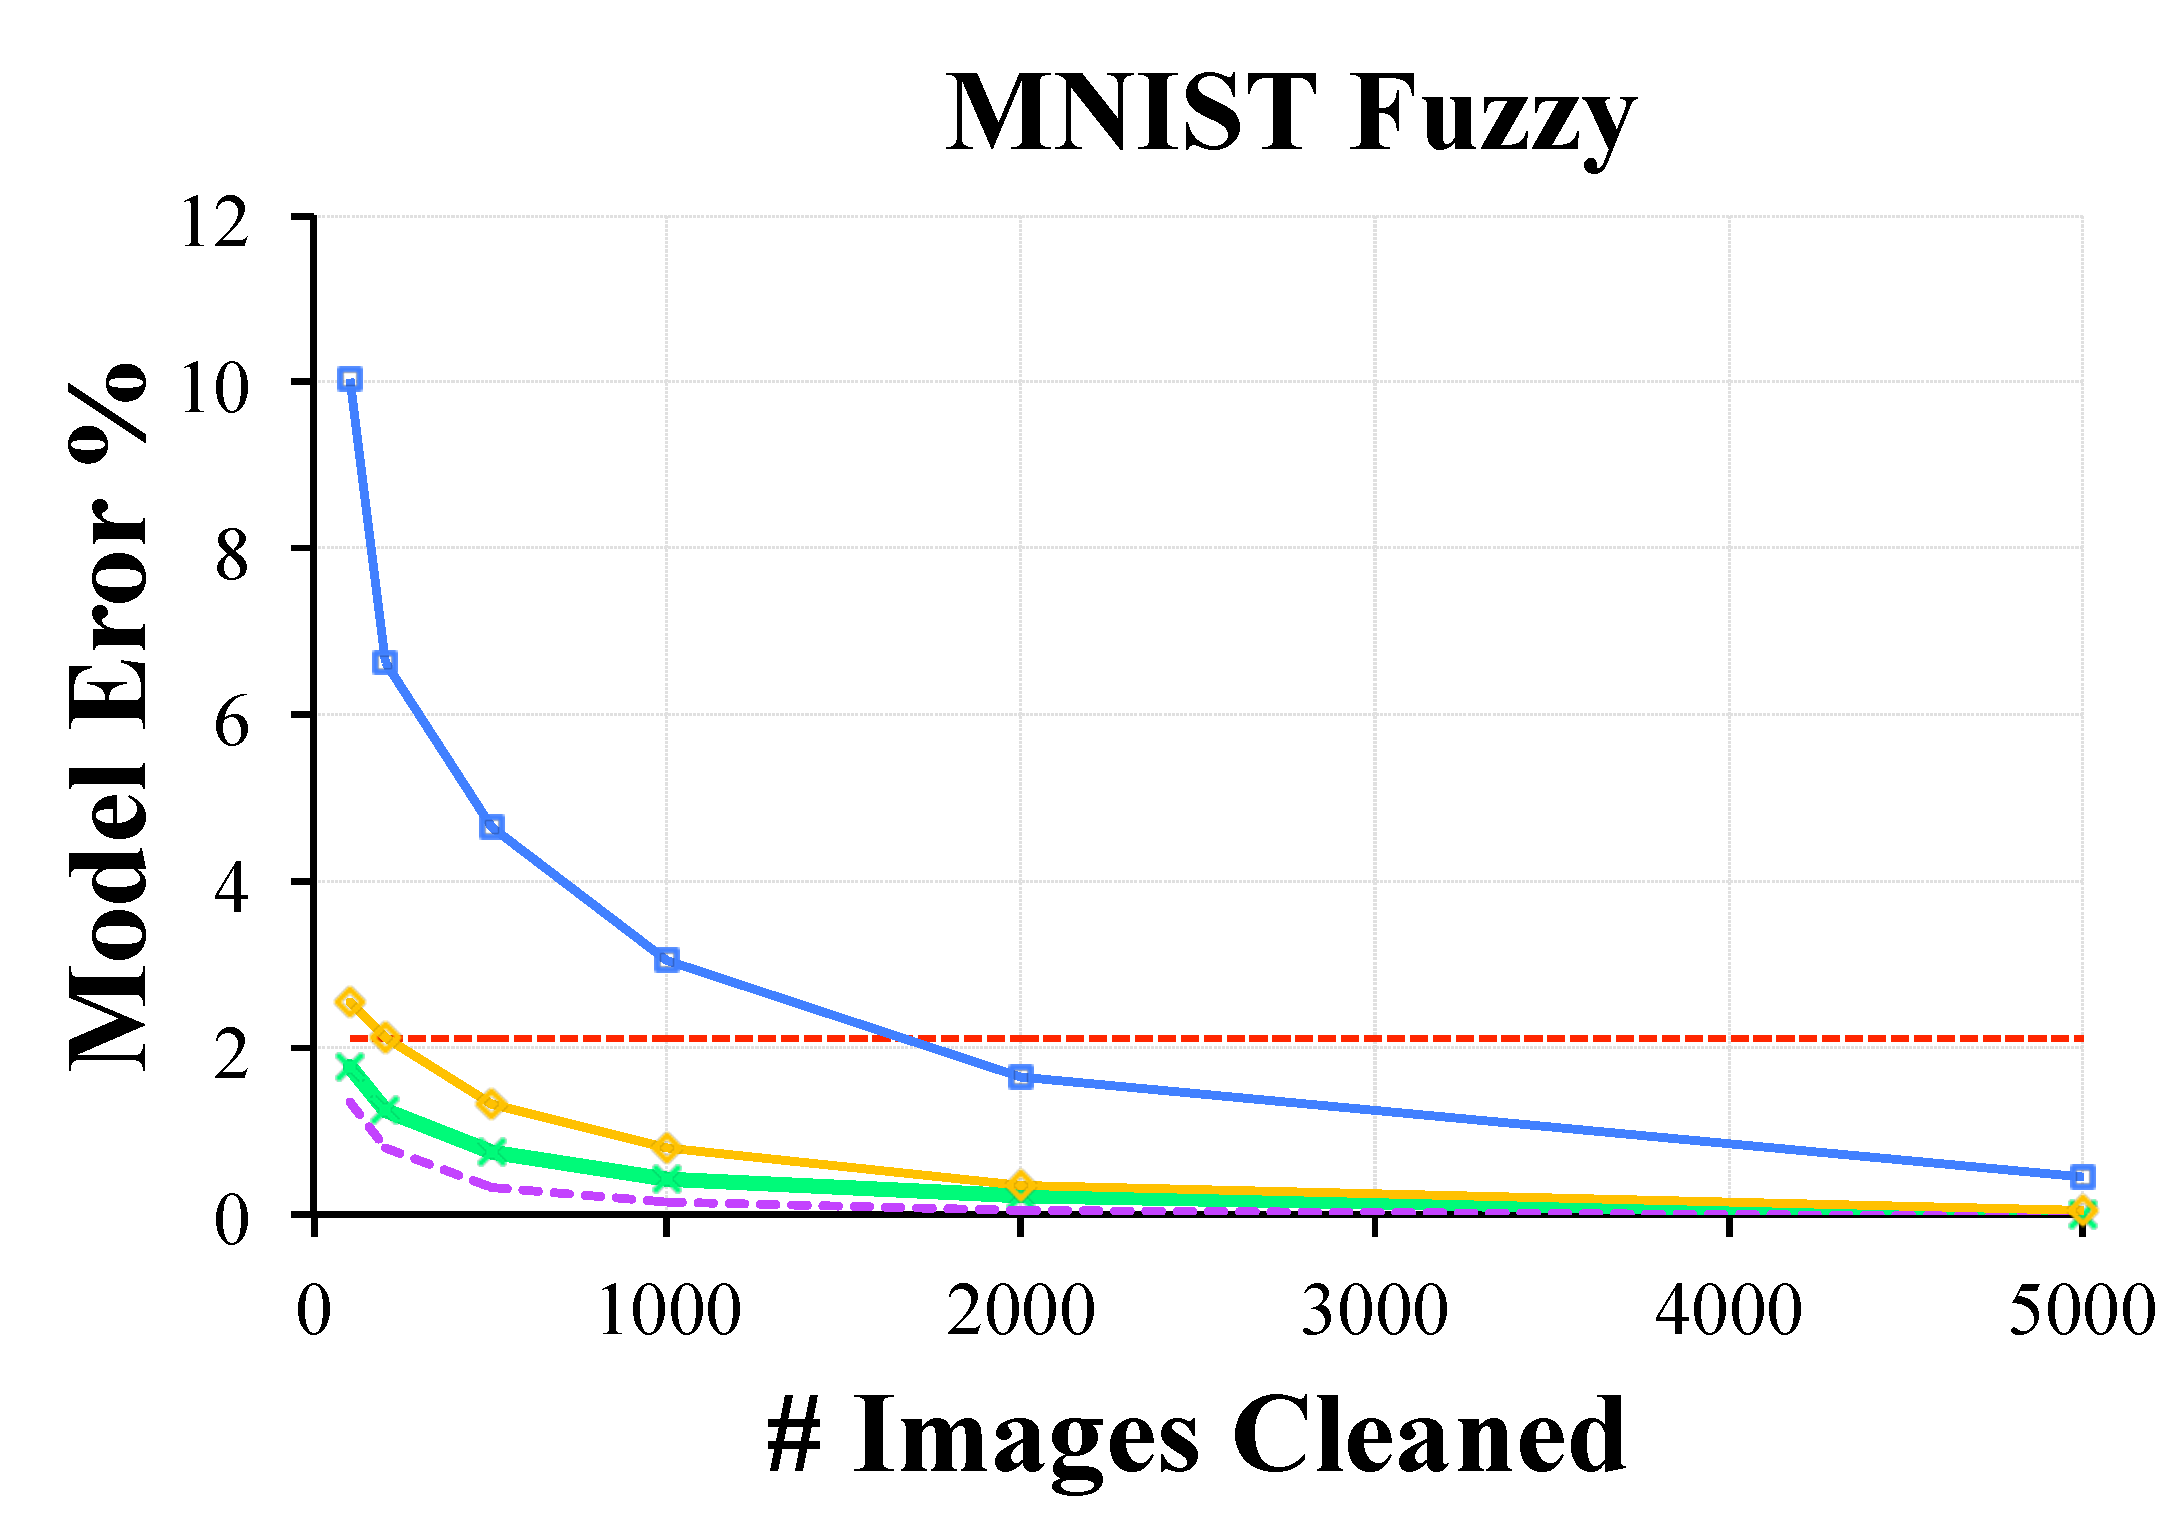
\includegraphics[width=0.49\columnwidth]{exp/exp7b.pdf}
 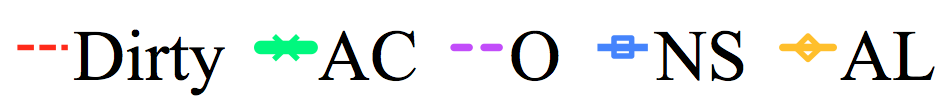
\includegraphics[width=0.49\columnwidth]{exp/legend-general.png}\vspace{-0.5em}
 \caption{In a real adaptive detection scenario with the MNIST dataset, \sys outperforms Active Learning and SampleClean.  \label{mnist}}
\end{figure}
